\subsection{Metriche}
I dati fanno riferimento a:
\begin{itemize}
	\item \textbf{Incremento:} incremento fra una fase ed un'altra, come definito all'interno del \PdPv{4.0.0};
	\item \textbf{A:} Fase di Analisi;
	\item \textbf{PA:} Fase di Progettazione Architetturale;
	\item \textbf{PD} Fase di Progettazione di Dettaglio e codifica;
	\item \textbf{VC: } Fase di Validazione e Collaudo.
\end{itemize}

\subsubsection{MPC1 - Percentuale di requisiti soddisfatti}
Di seguito è riportato il grafico dei requisiti soddisfatti, il cui valore è definito accettabile e ottimale come descritto nella sezione §2.1.1.1.\\

\begin{figure}[H]
\centering
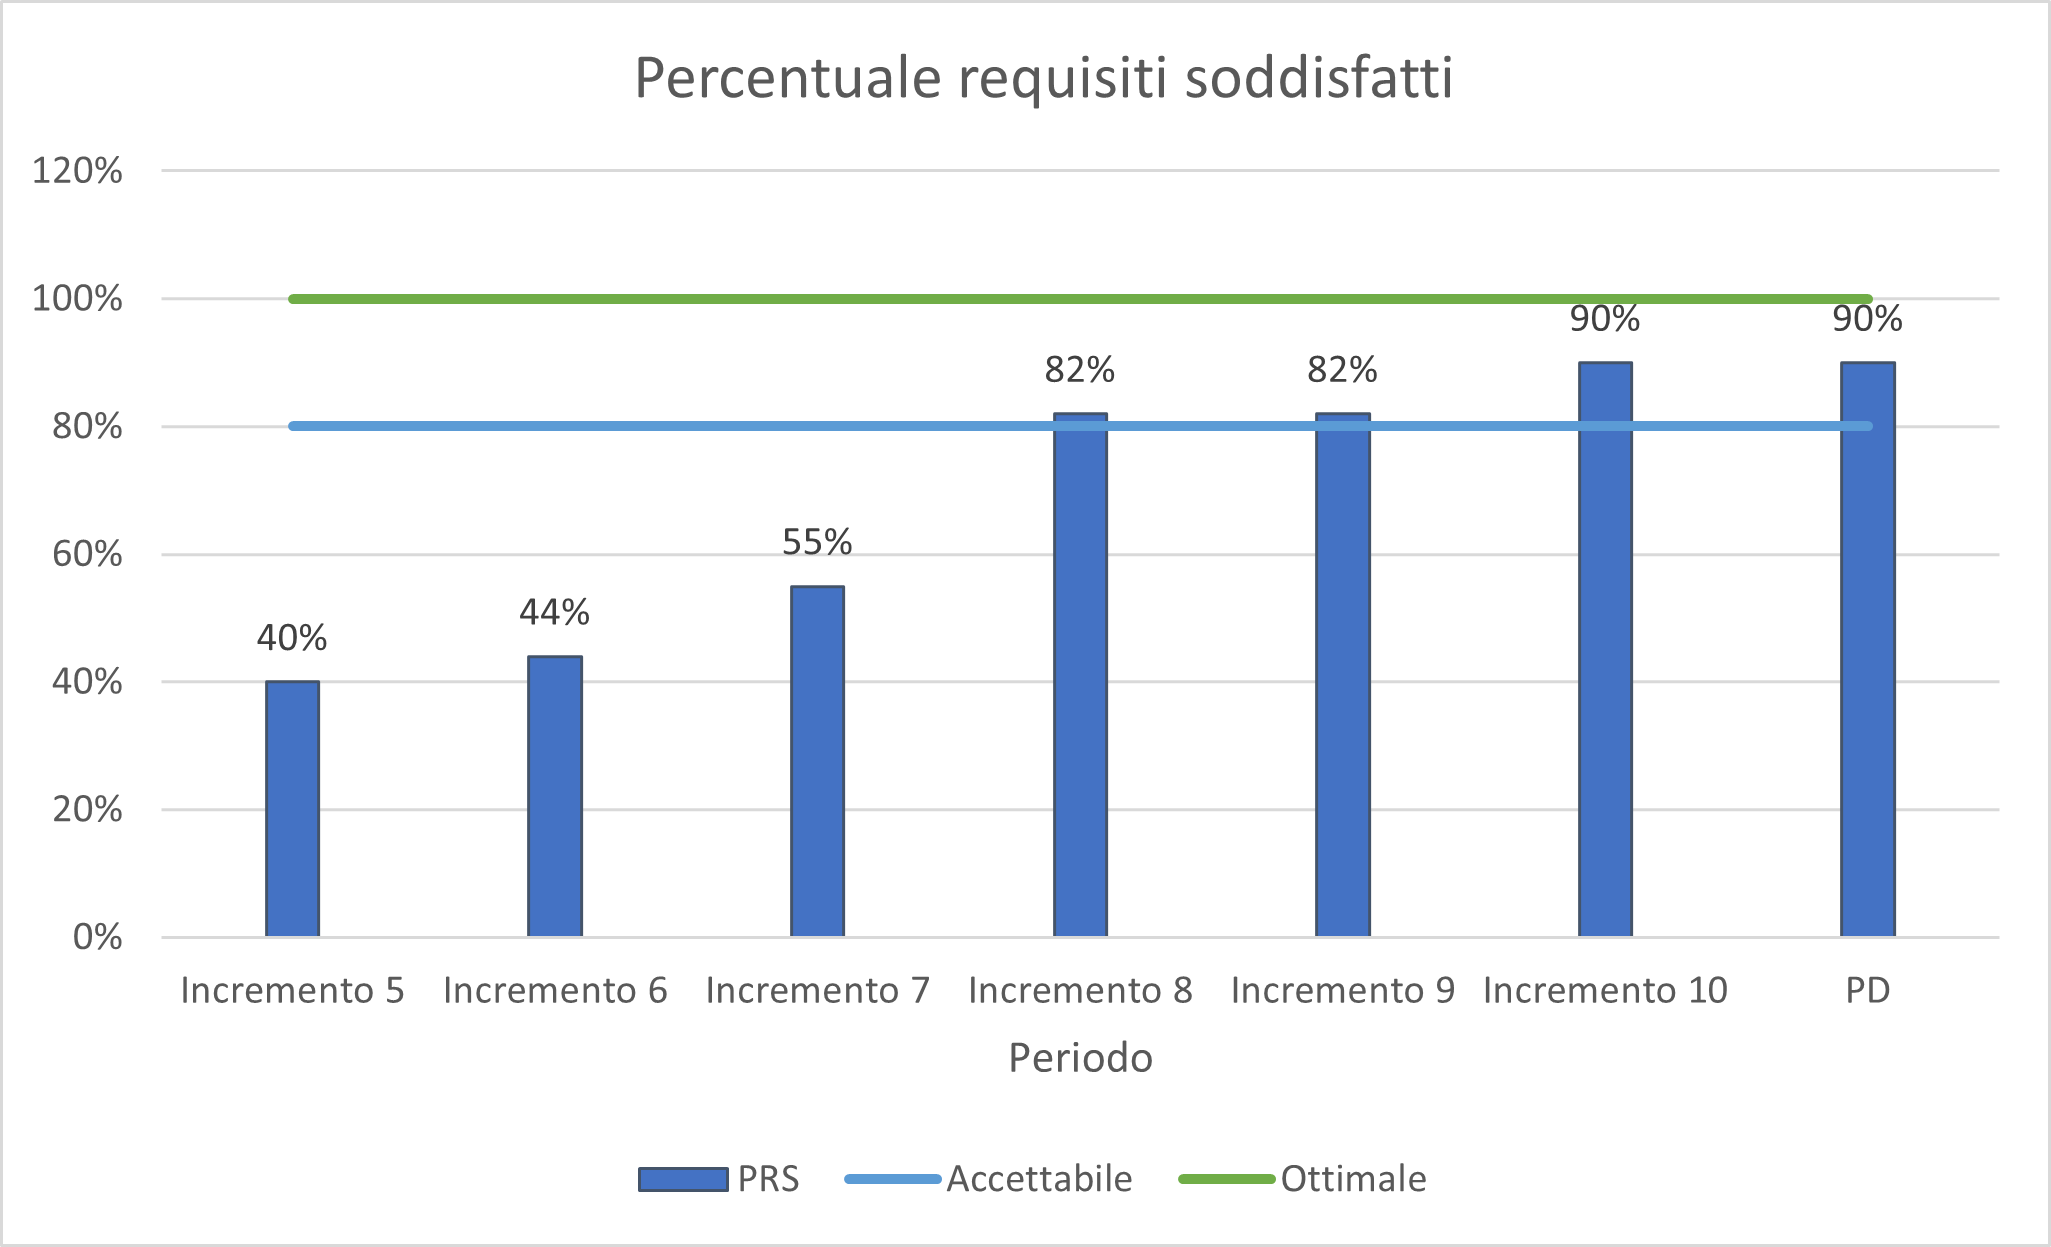
\includegraphics[scale=0.78]{res/ResocontoAttivitaDiVerifica/res/metriche/grafici/img/PRS.png}\\
\caption{Andamento percentuale di requisiti soddisfatti}
\end{figure}

\subsubsection{MPC2 - Percentuale di requisiti obbligatori soddisfatti}
Di seguito è riportato il grafico dei requisiti obbligatori soddisfatti, il cui valore è definito accettabile e ottimale come descritto nella sezione §2.1.1.2.\\

\begin{figure}[H]
\centering
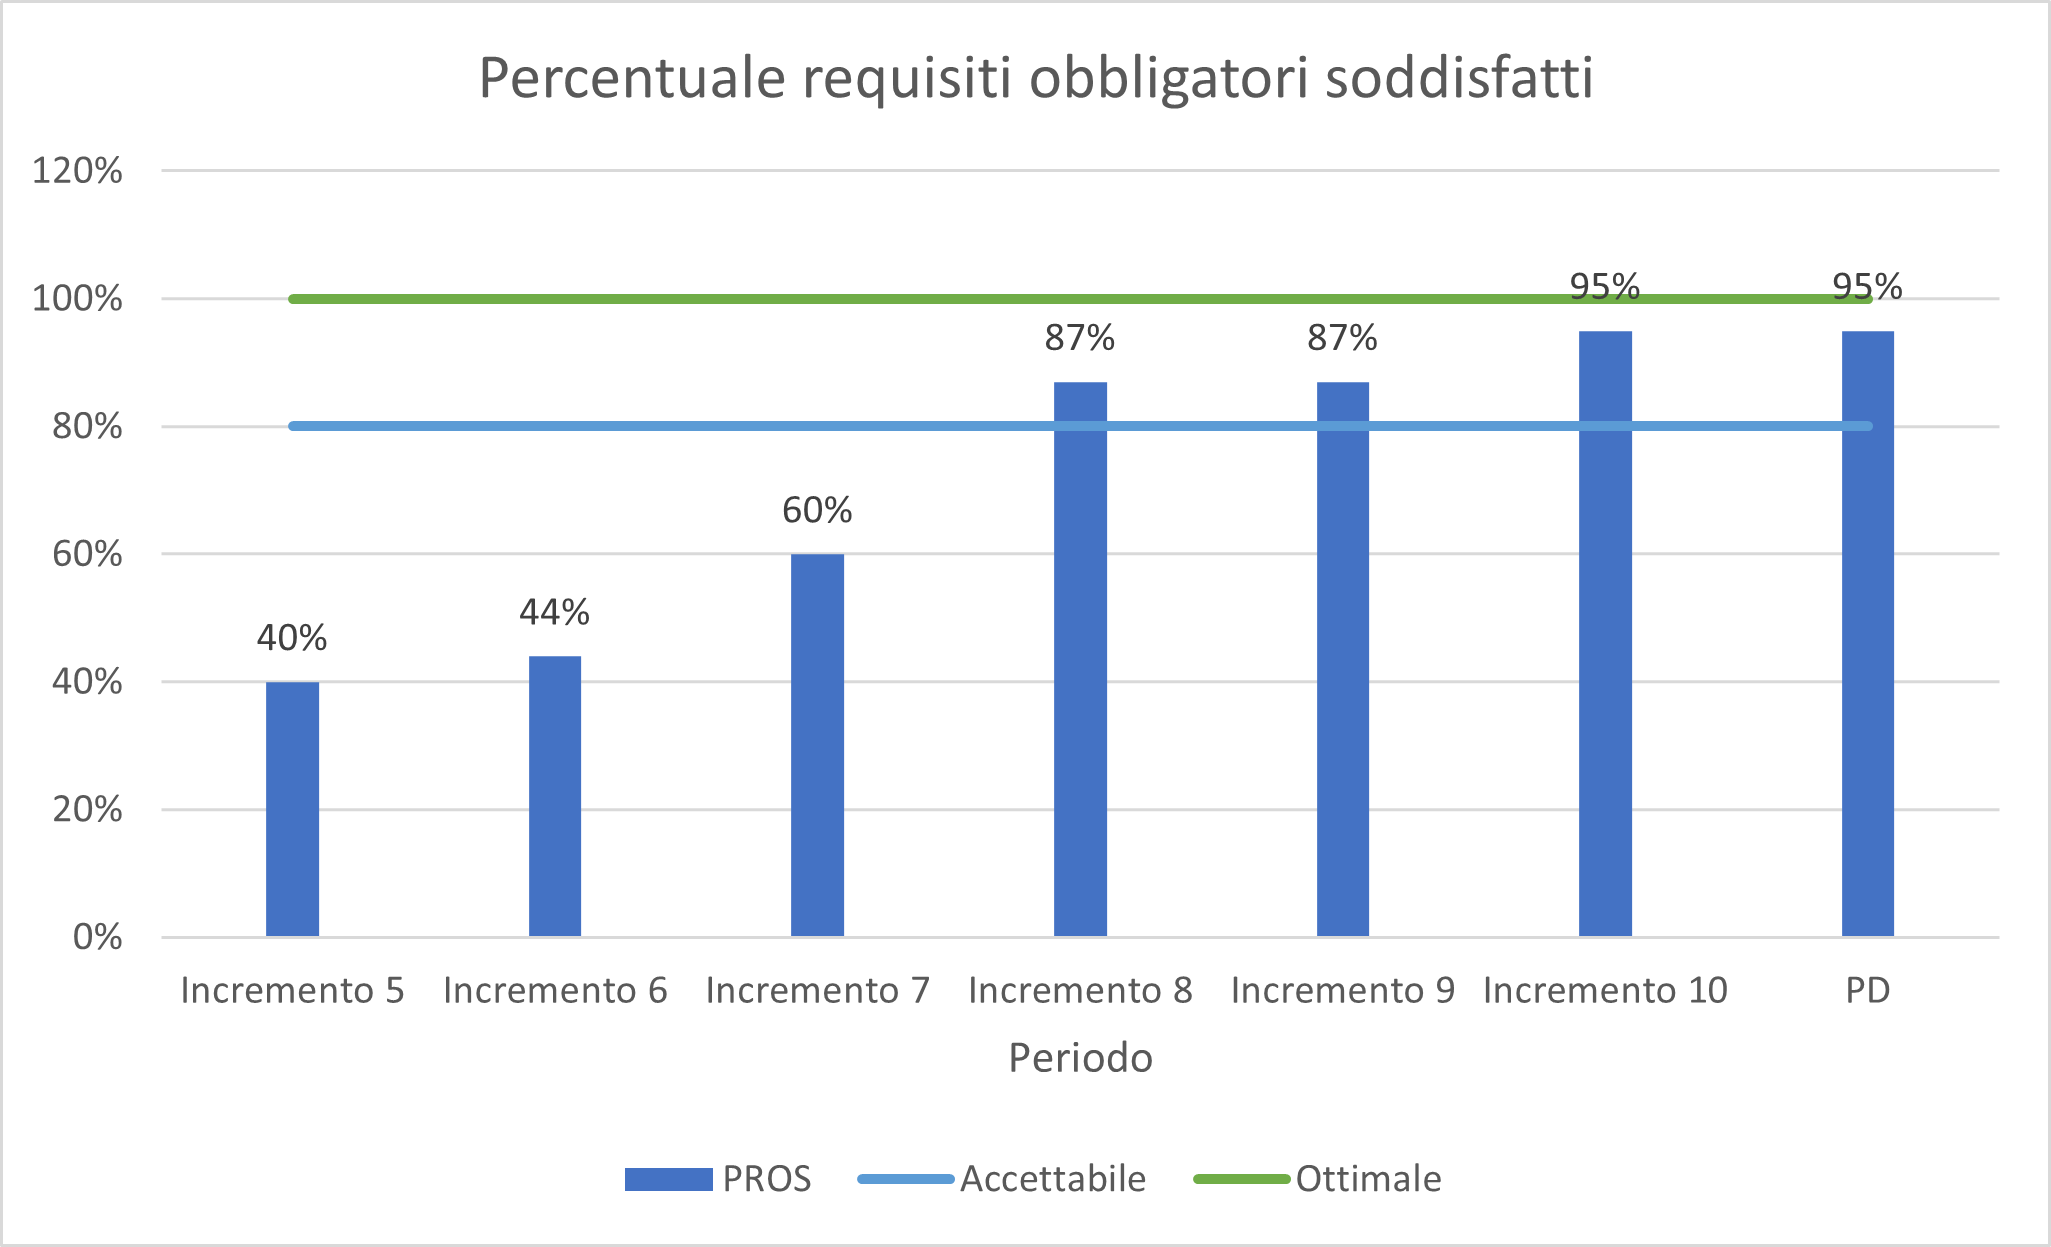
\includegraphics[scale=0.78]{res/ResocontoAttivitaDiVerifica/res/metriche/grafici/img/PROS.png}\\
\caption{Andamento percentuale di requisiti obbligatori soddisfatti}
\end{figure}

\subsection{Esiti delle verifiche dell'indice di Gulpease}
Di seguito è riportato il grafico dell'indice di Gulpease calcolato sui vari documenti, il cui valore è definito accettabile e ottimale come descritto nella sezione §2.2.1.1.\\
I dati fanno riferimento a:
\begin{itemize}
	\item \textbf{RR:} Revisione dei Requisiti;
	\item \textbf{RP:} Revisione di Progettazione;
	\item \textbf{RQ:} Revisione di Qualifica (da aggiungere con l'avanzare del progetto);
	\item \textbf{RA:} Revisione di Accettazione (da aggiungere con l'avanzare del progetto).
\end{itemize} 

\subsubsection{Grafico complessivo}

\begin{figure}[H]
\centering
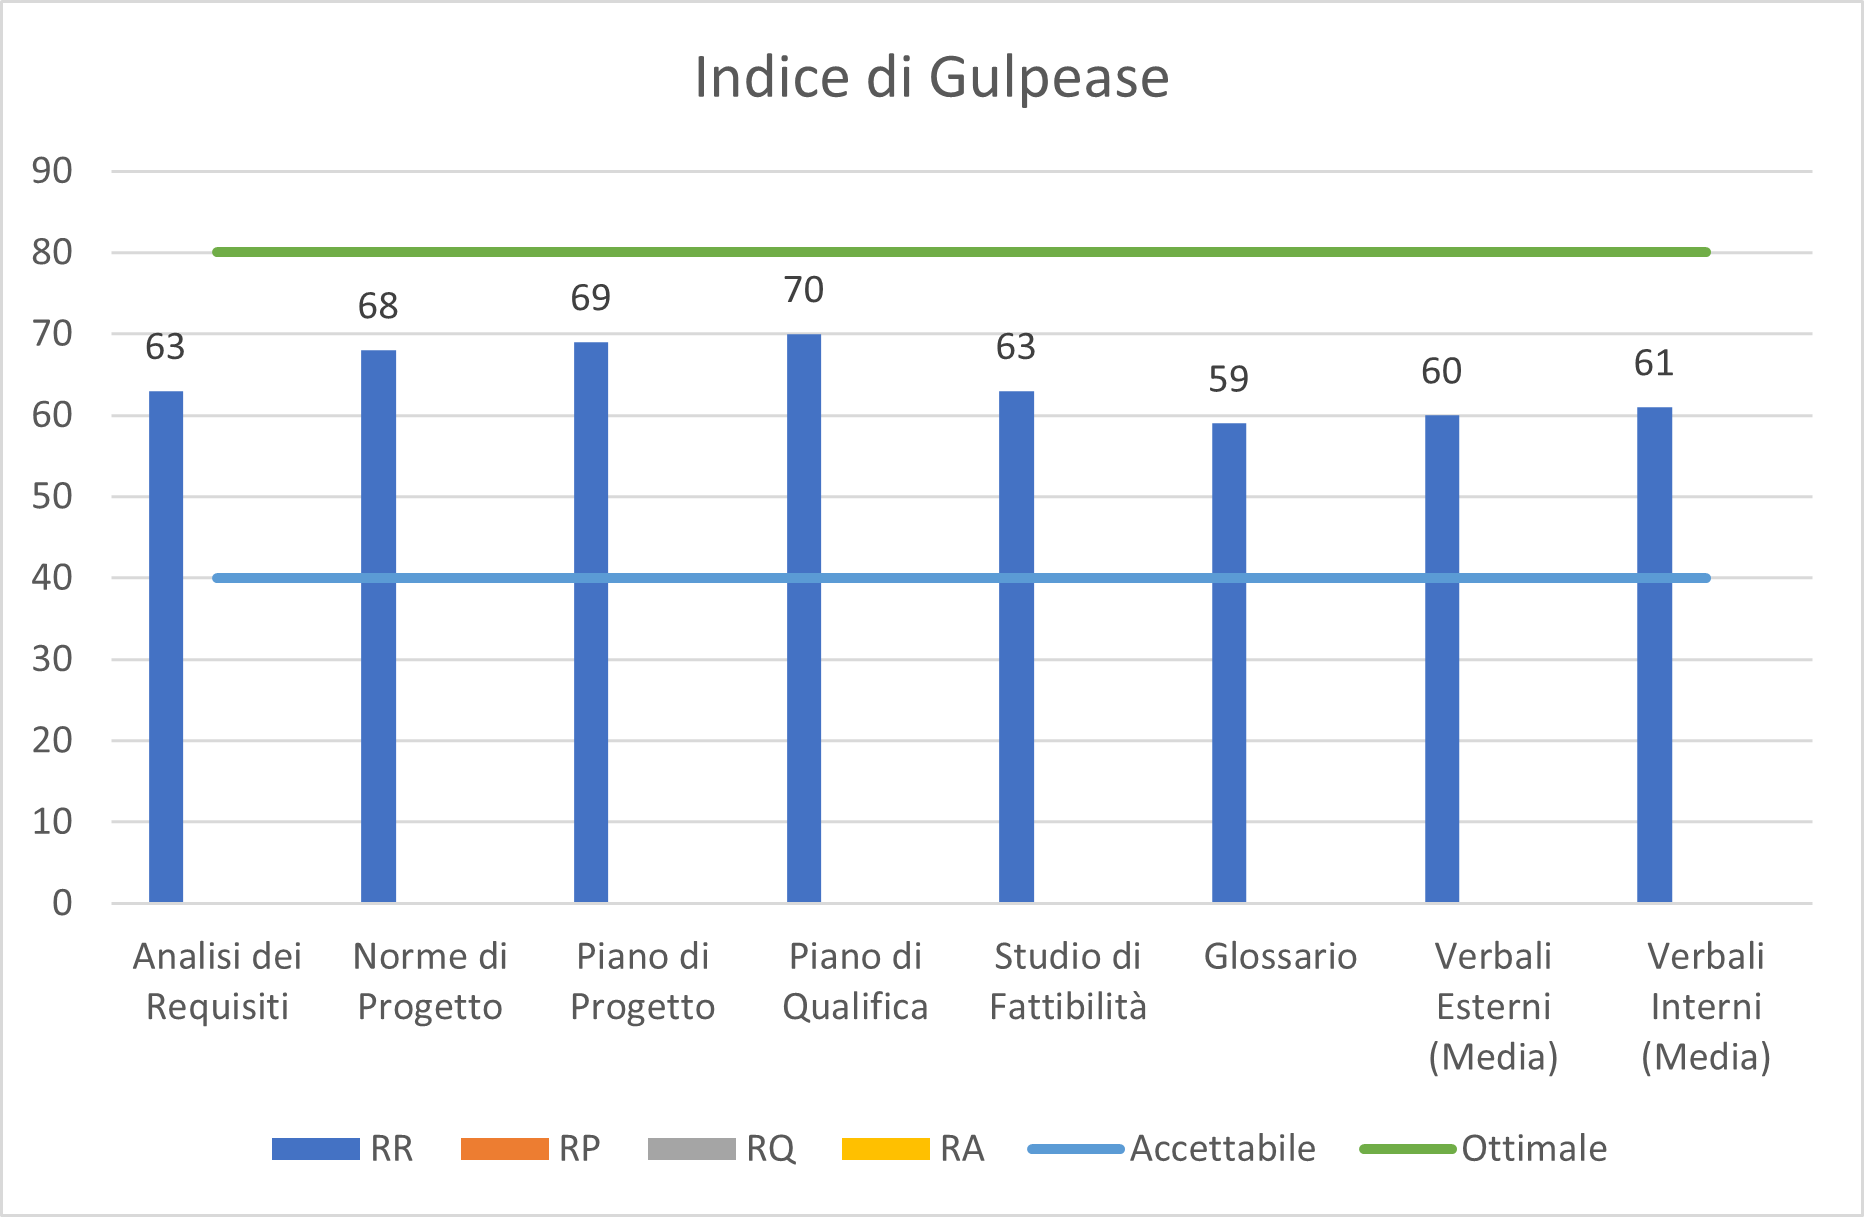
\includegraphics[scale=0.90]{res/ResocontoAttivitaDiVerifica/res/img/indiceGulpease.png}\\
\caption{Andamento complessivo dell'indice di Gulpease}
\end{figure}

\subsubsection{Grafico per documento}

\begin{figure}[H]
\centering
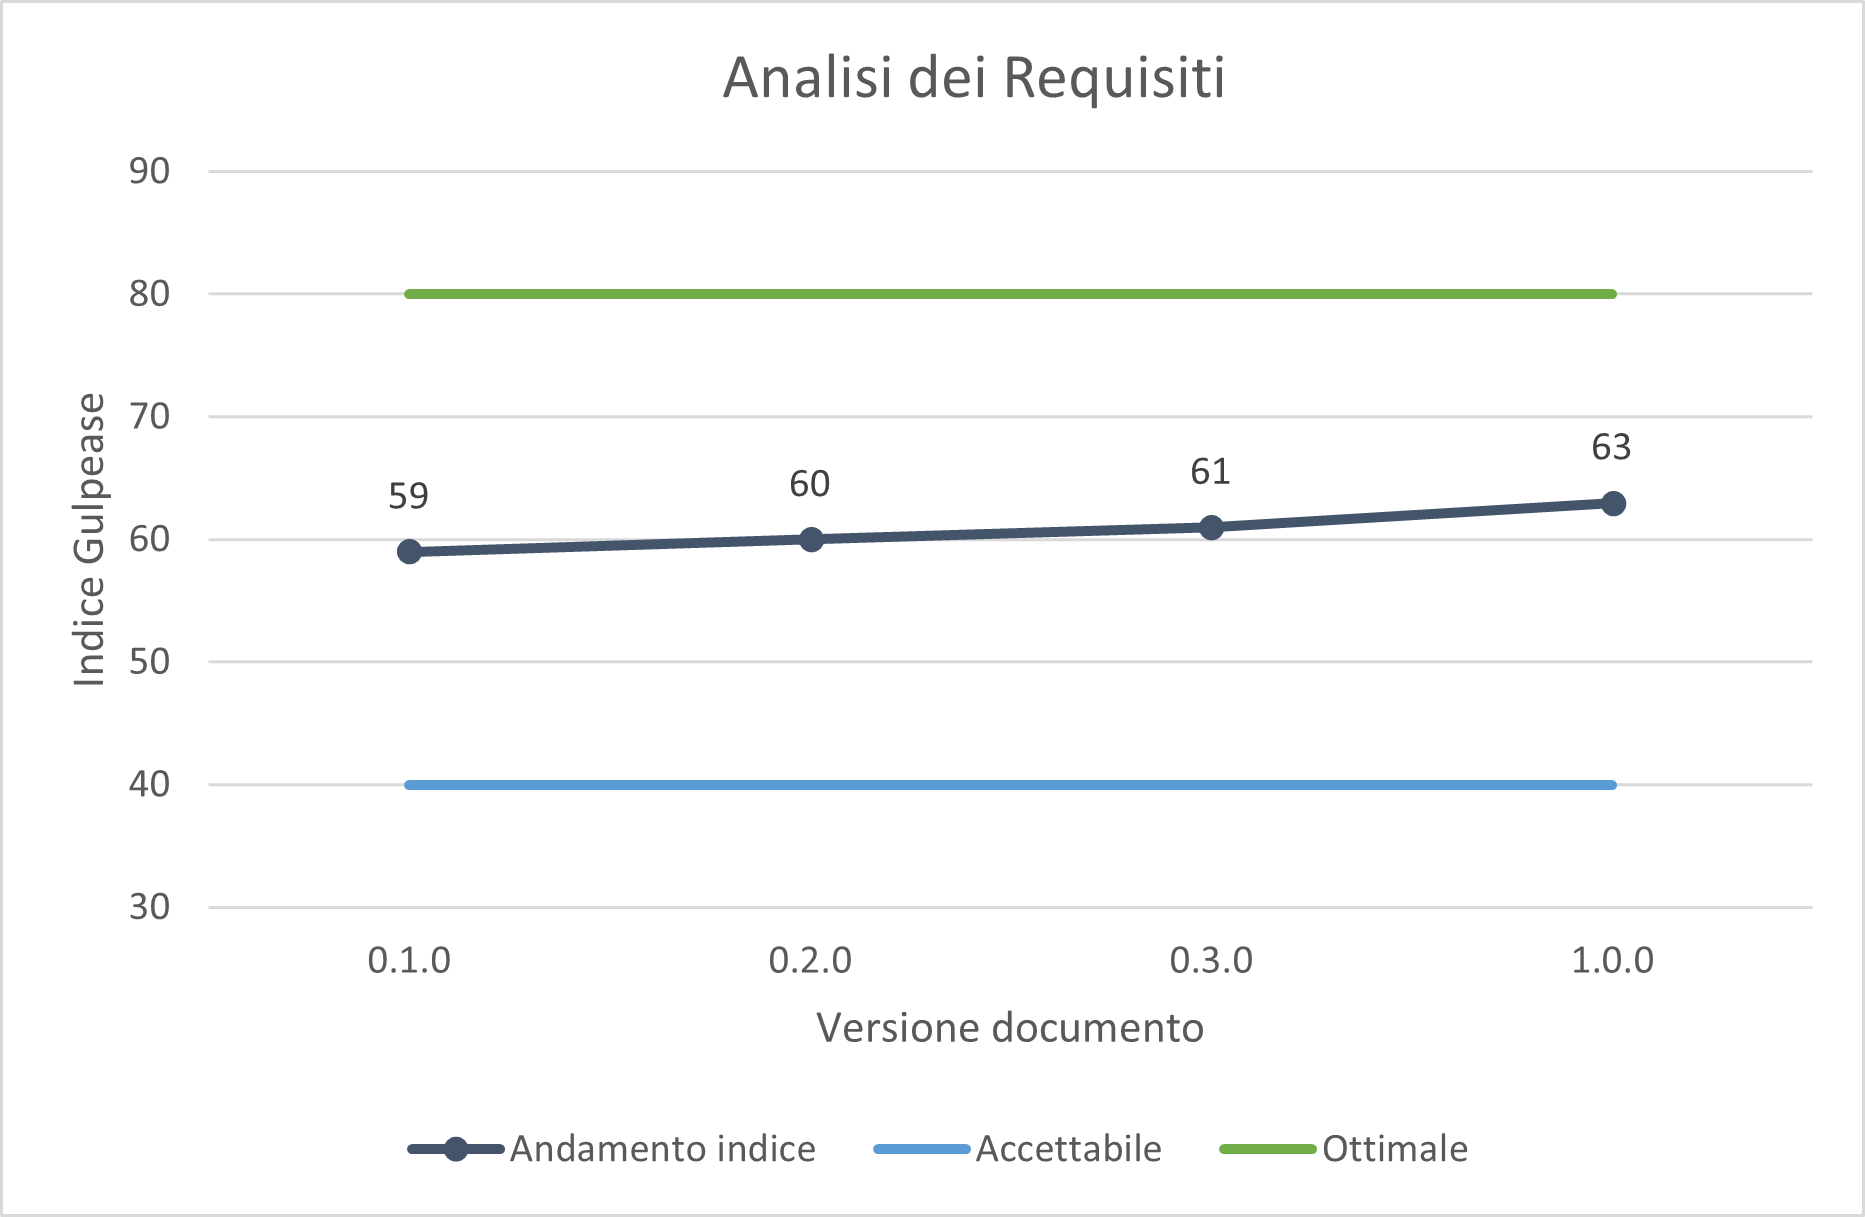
\includegraphics[scale=0.90]{res/ResocontoAttivitaDiVerifica/res/img/gulpeaseADR.png}\\
\caption{Andamento dell'indice di Gulpease \AdR}
\end{figure}

\begin{figure}[H]
\centering
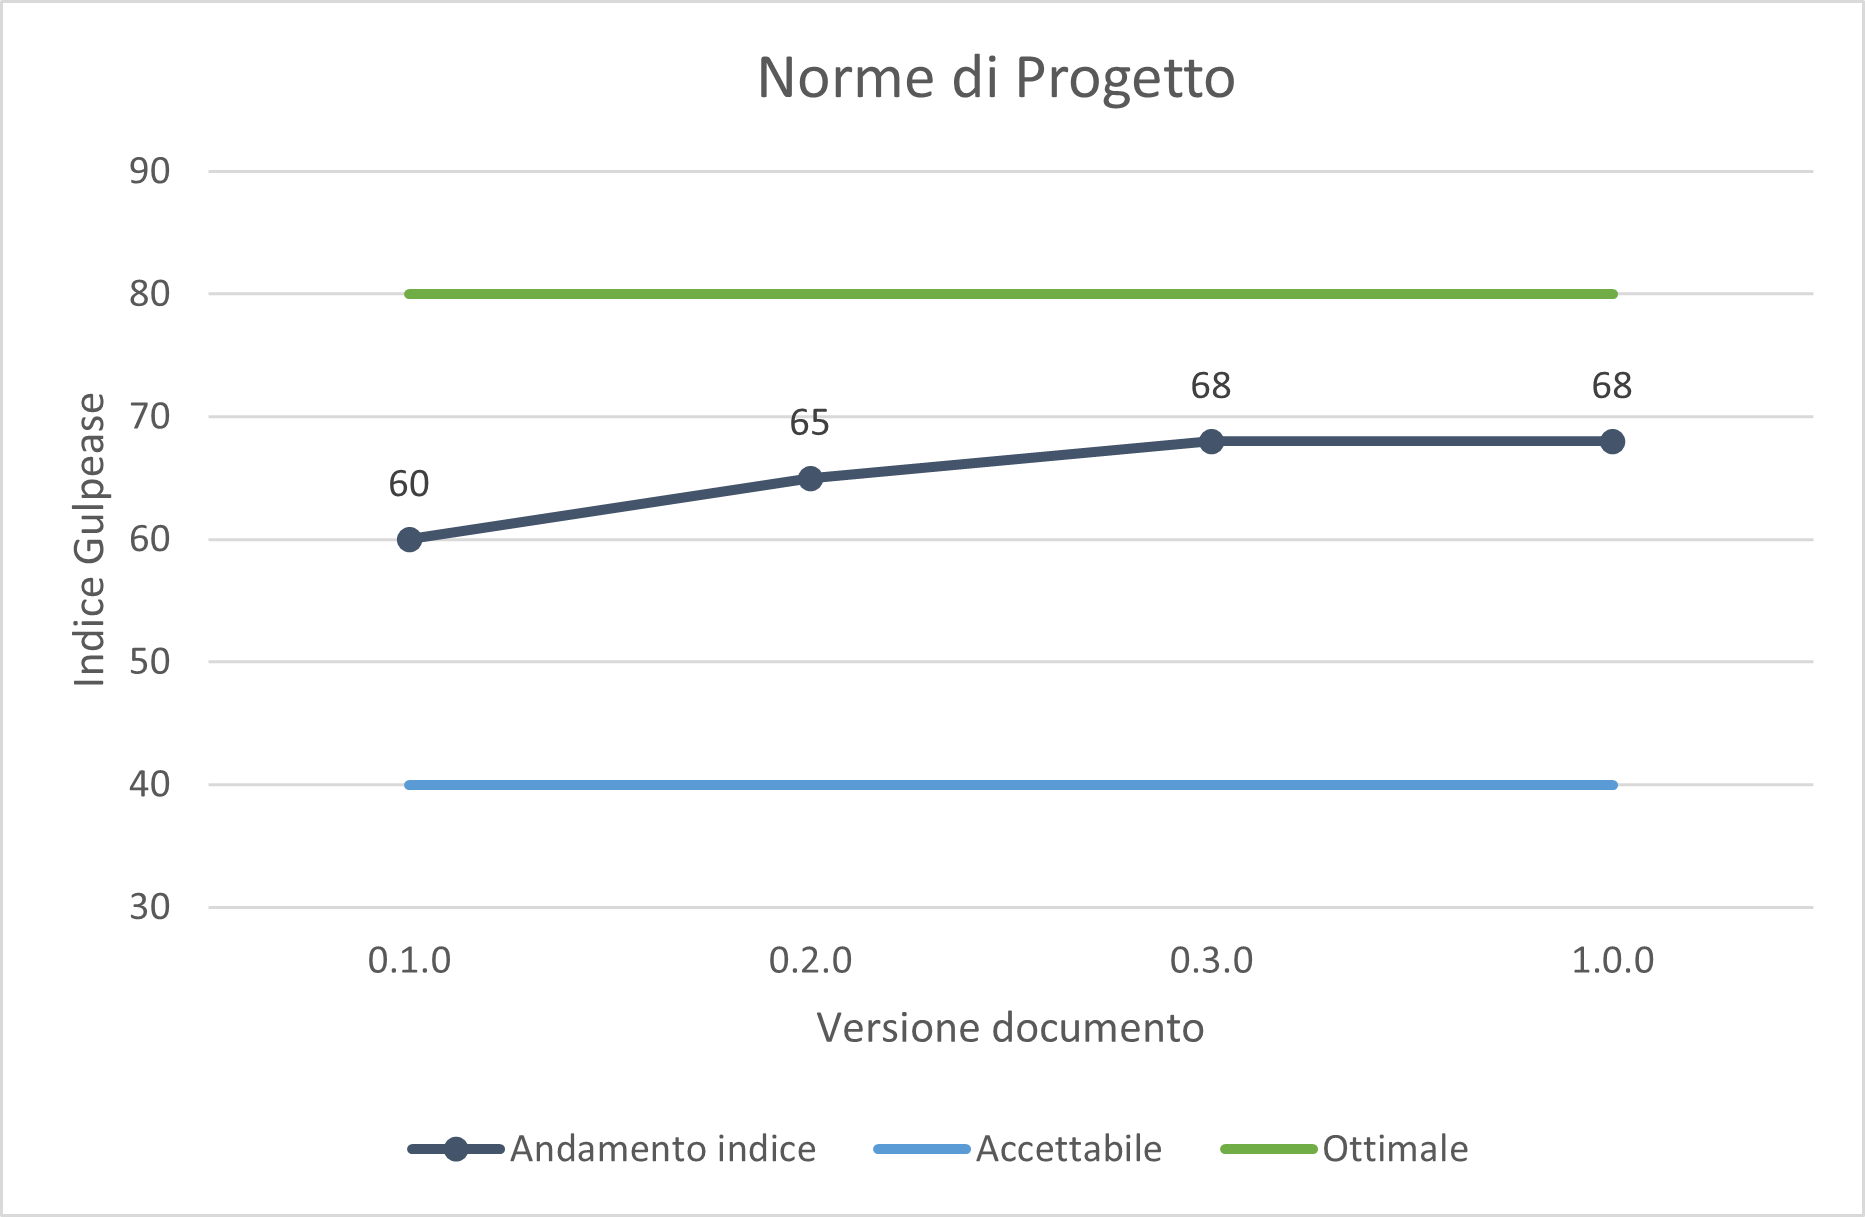
\includegraphics[scale=0.90]{res/ResocontoAttivitaDiVerifica/res/img/gulpeaseNDP.png}\\
\caption{Andamento dell'indice di Gulpease \NdP}
\end{figure}

\begin{figure}[H]
\centering
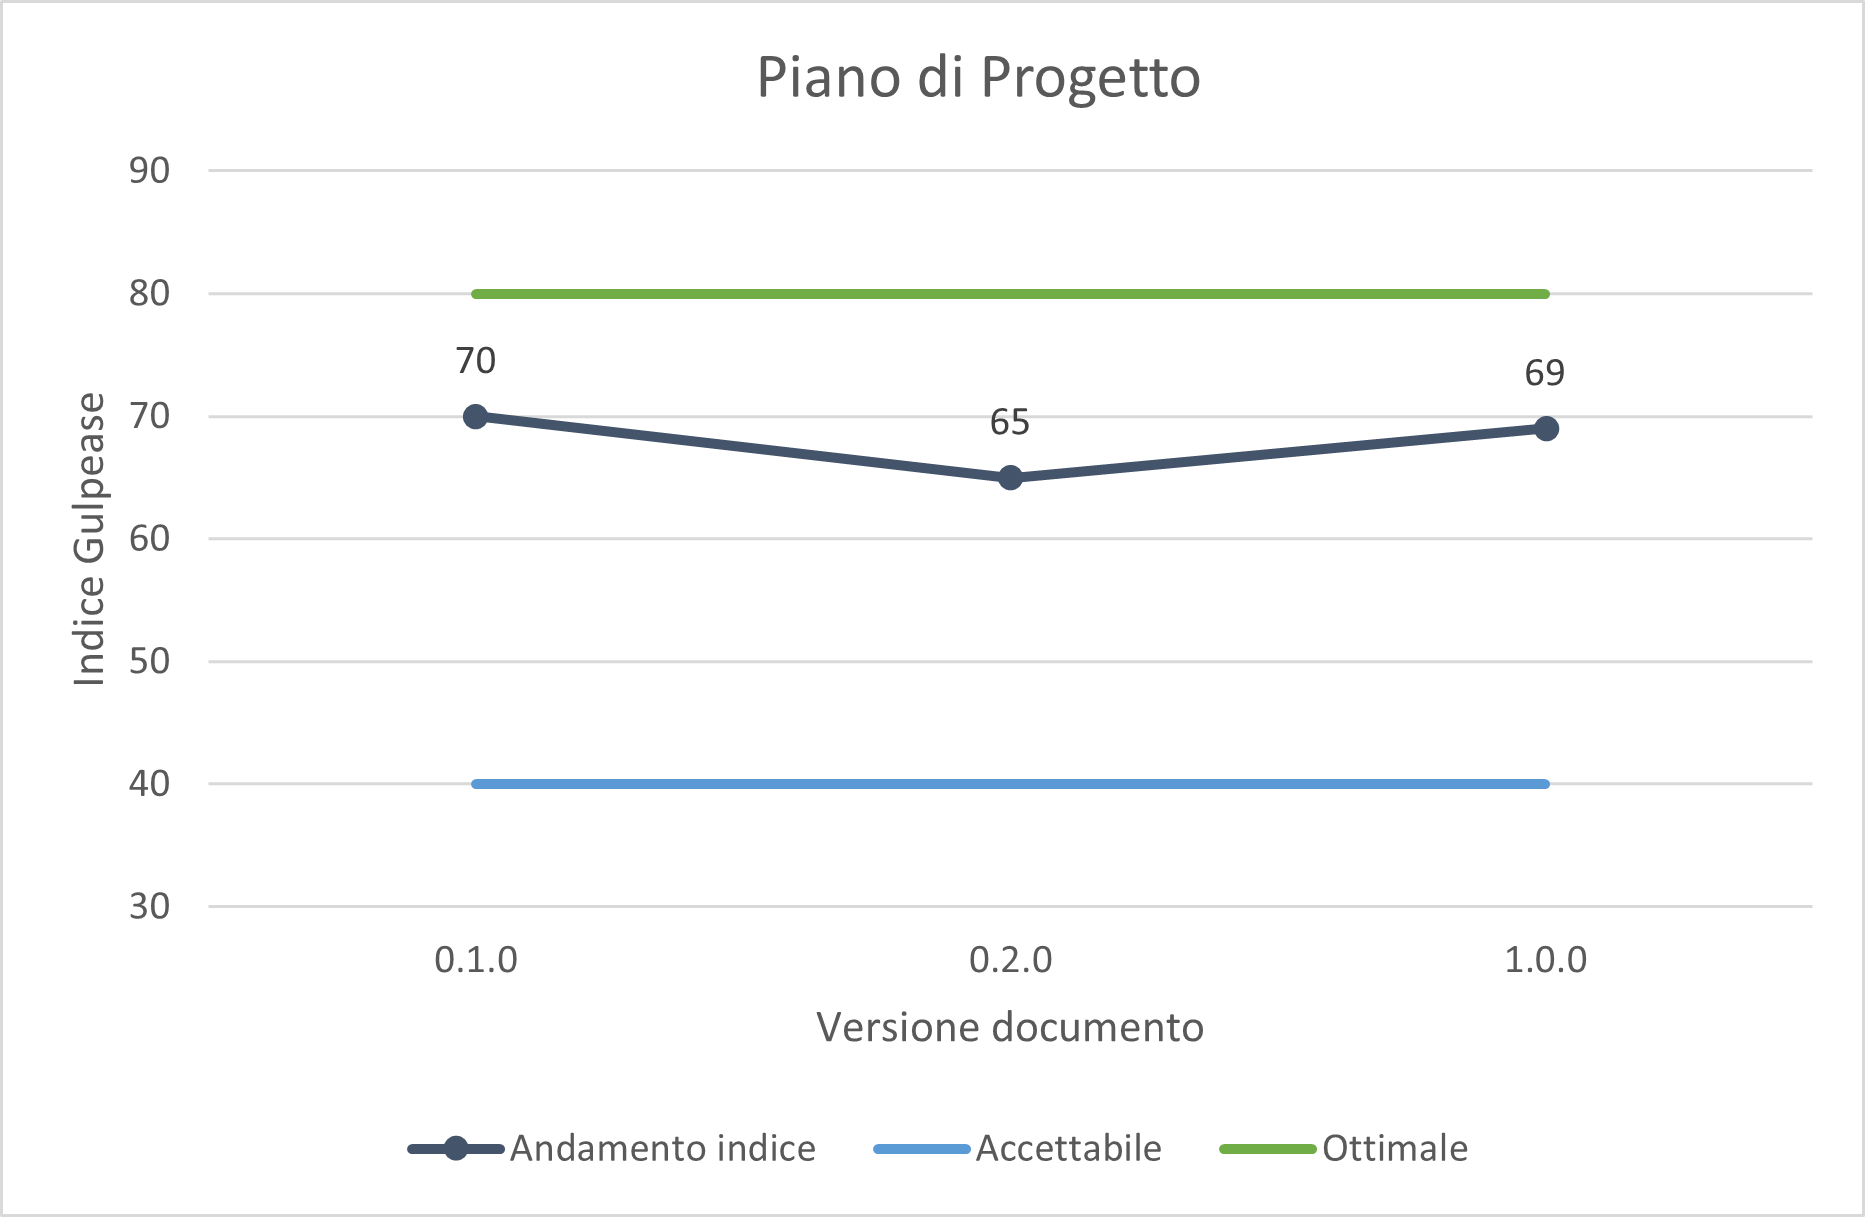
\includegraphics[scale=0.90]{res/ResocontoAttivitaDiVerifica/res/img/gulpeasePDP.png}\\
\caption{Andamento dell'indice di Gulpease \PdP}
\end{figure}

\begin{figure}[H]
\centering
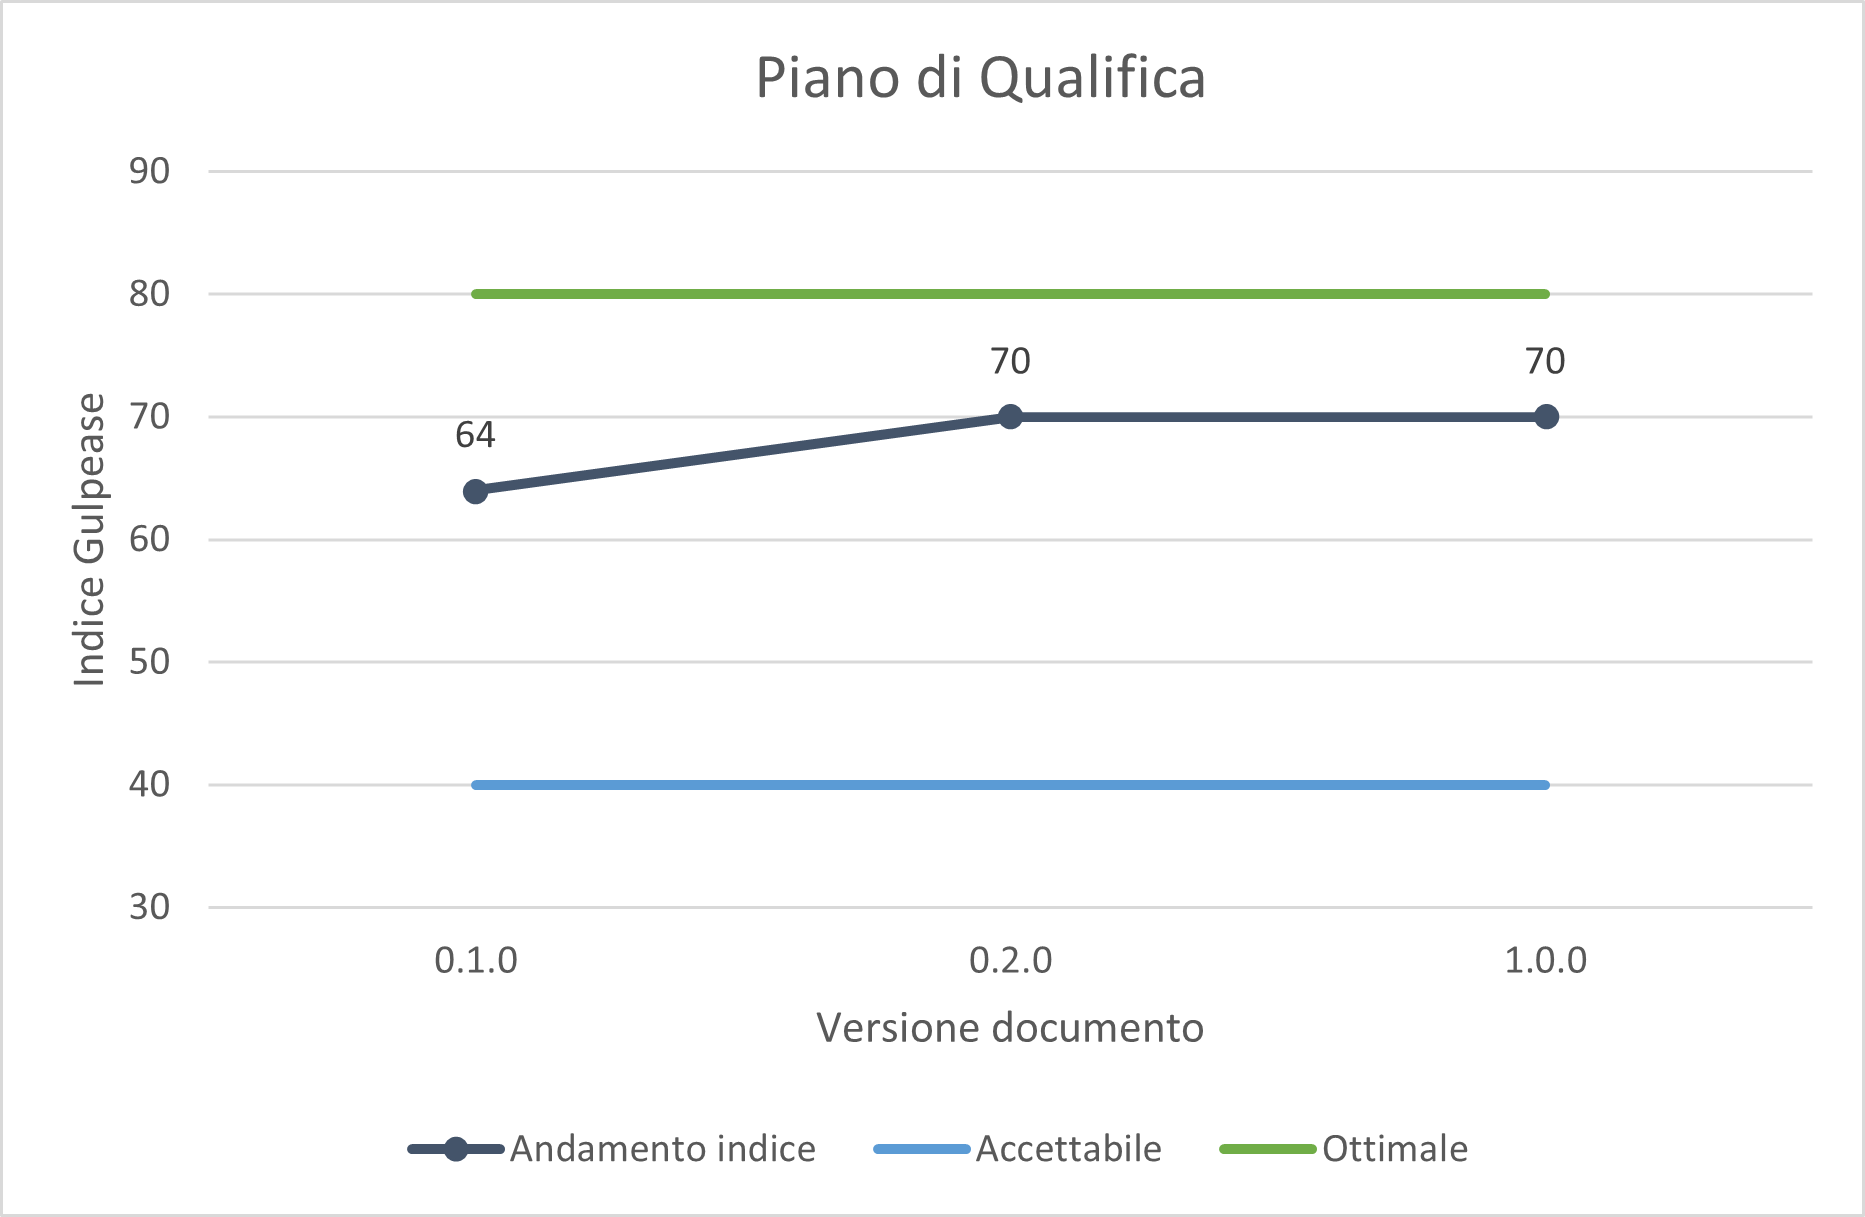
\includegraphics[scale=0.90]{res/ResocontoAttivitaDiVerifica/res/img/gulpeasePDQ.png}\\
\caption{Andamento dell'indice di Gulpease \PdQ}
\end{figure}

\begin{figure}[H]
\centering
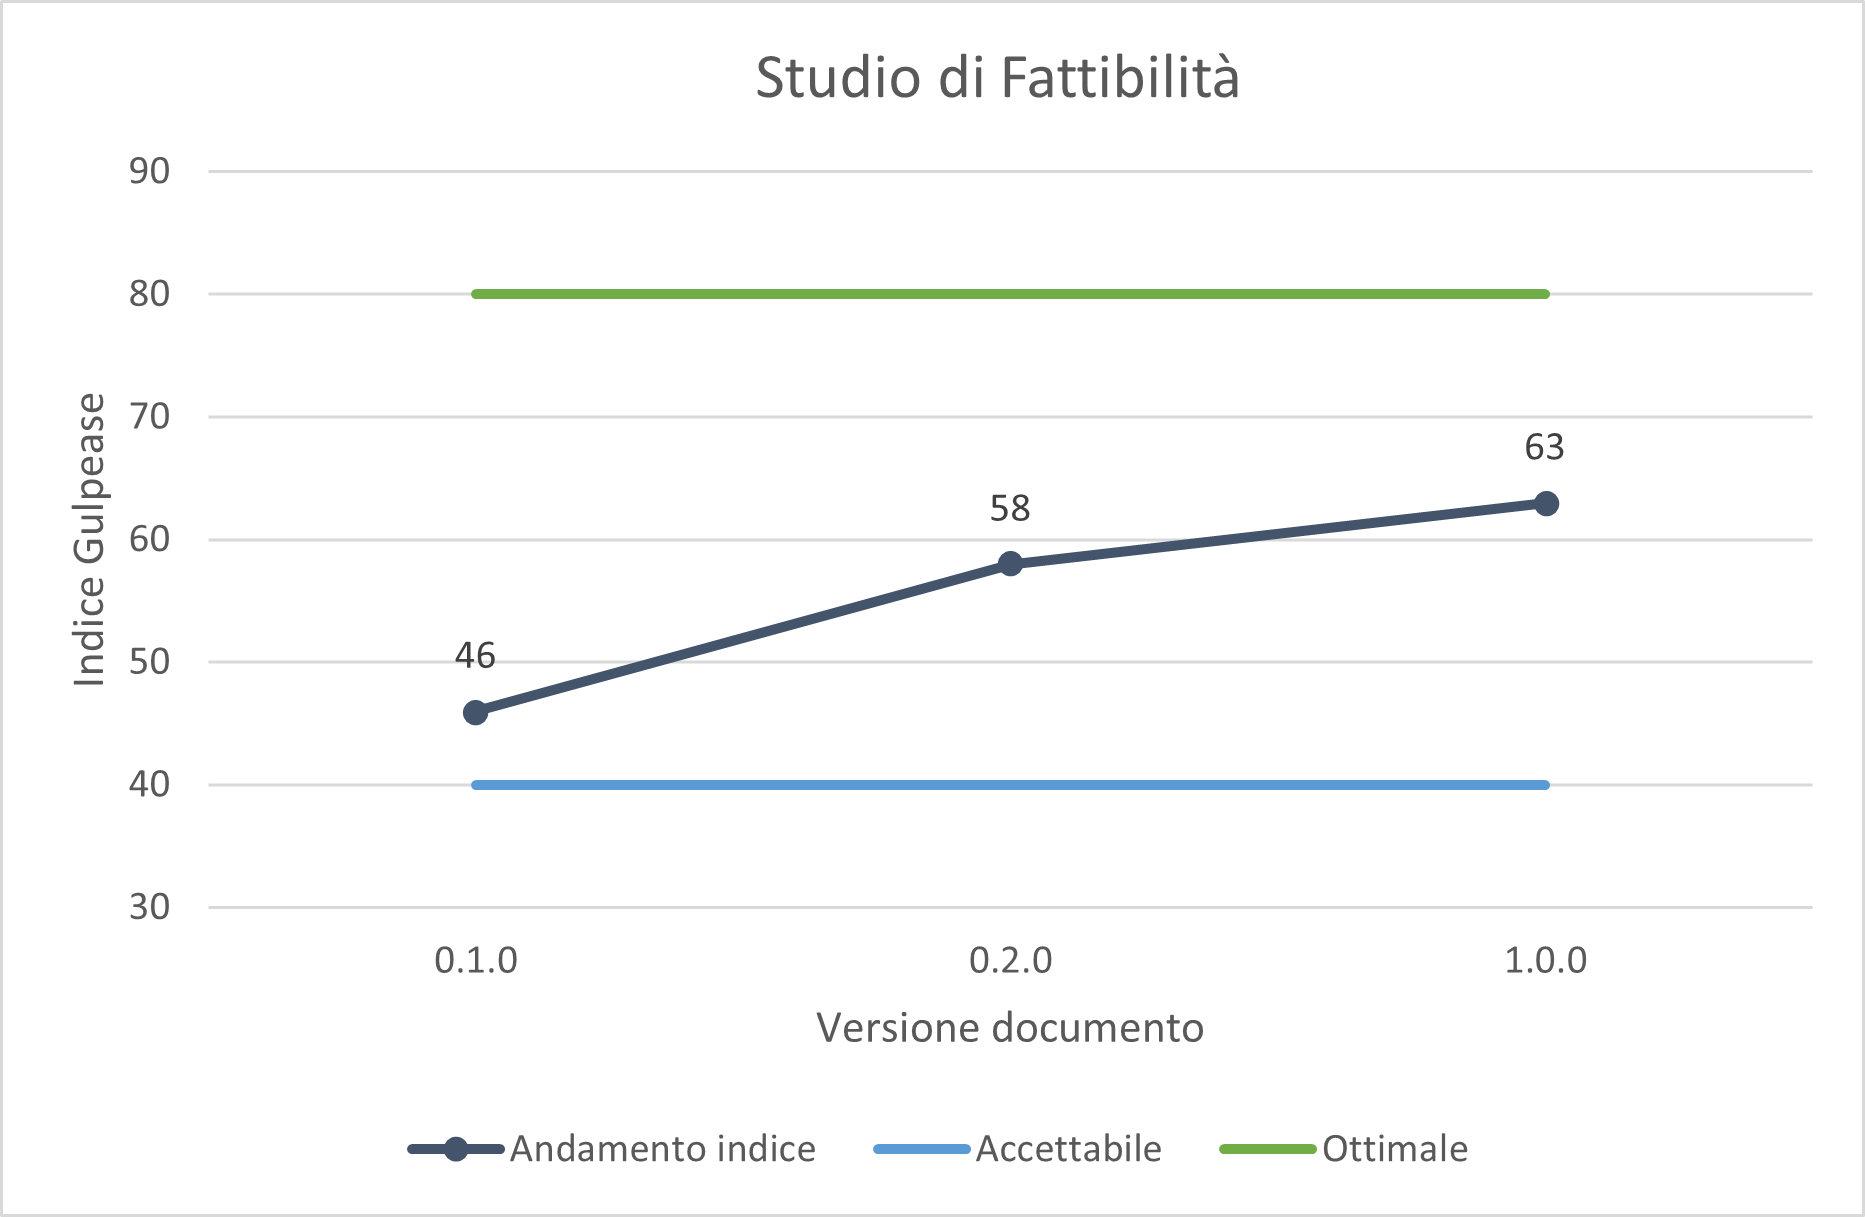
\includegraphics[scale=0.90]{res/ResocontoAttivitaDiVerifica/res/img/gulpeaseSDF.png}\\
\caption{Andamento dell'indice di Gulpease \SdF}
\end{figure}

\begin{figure}[H]
\centering
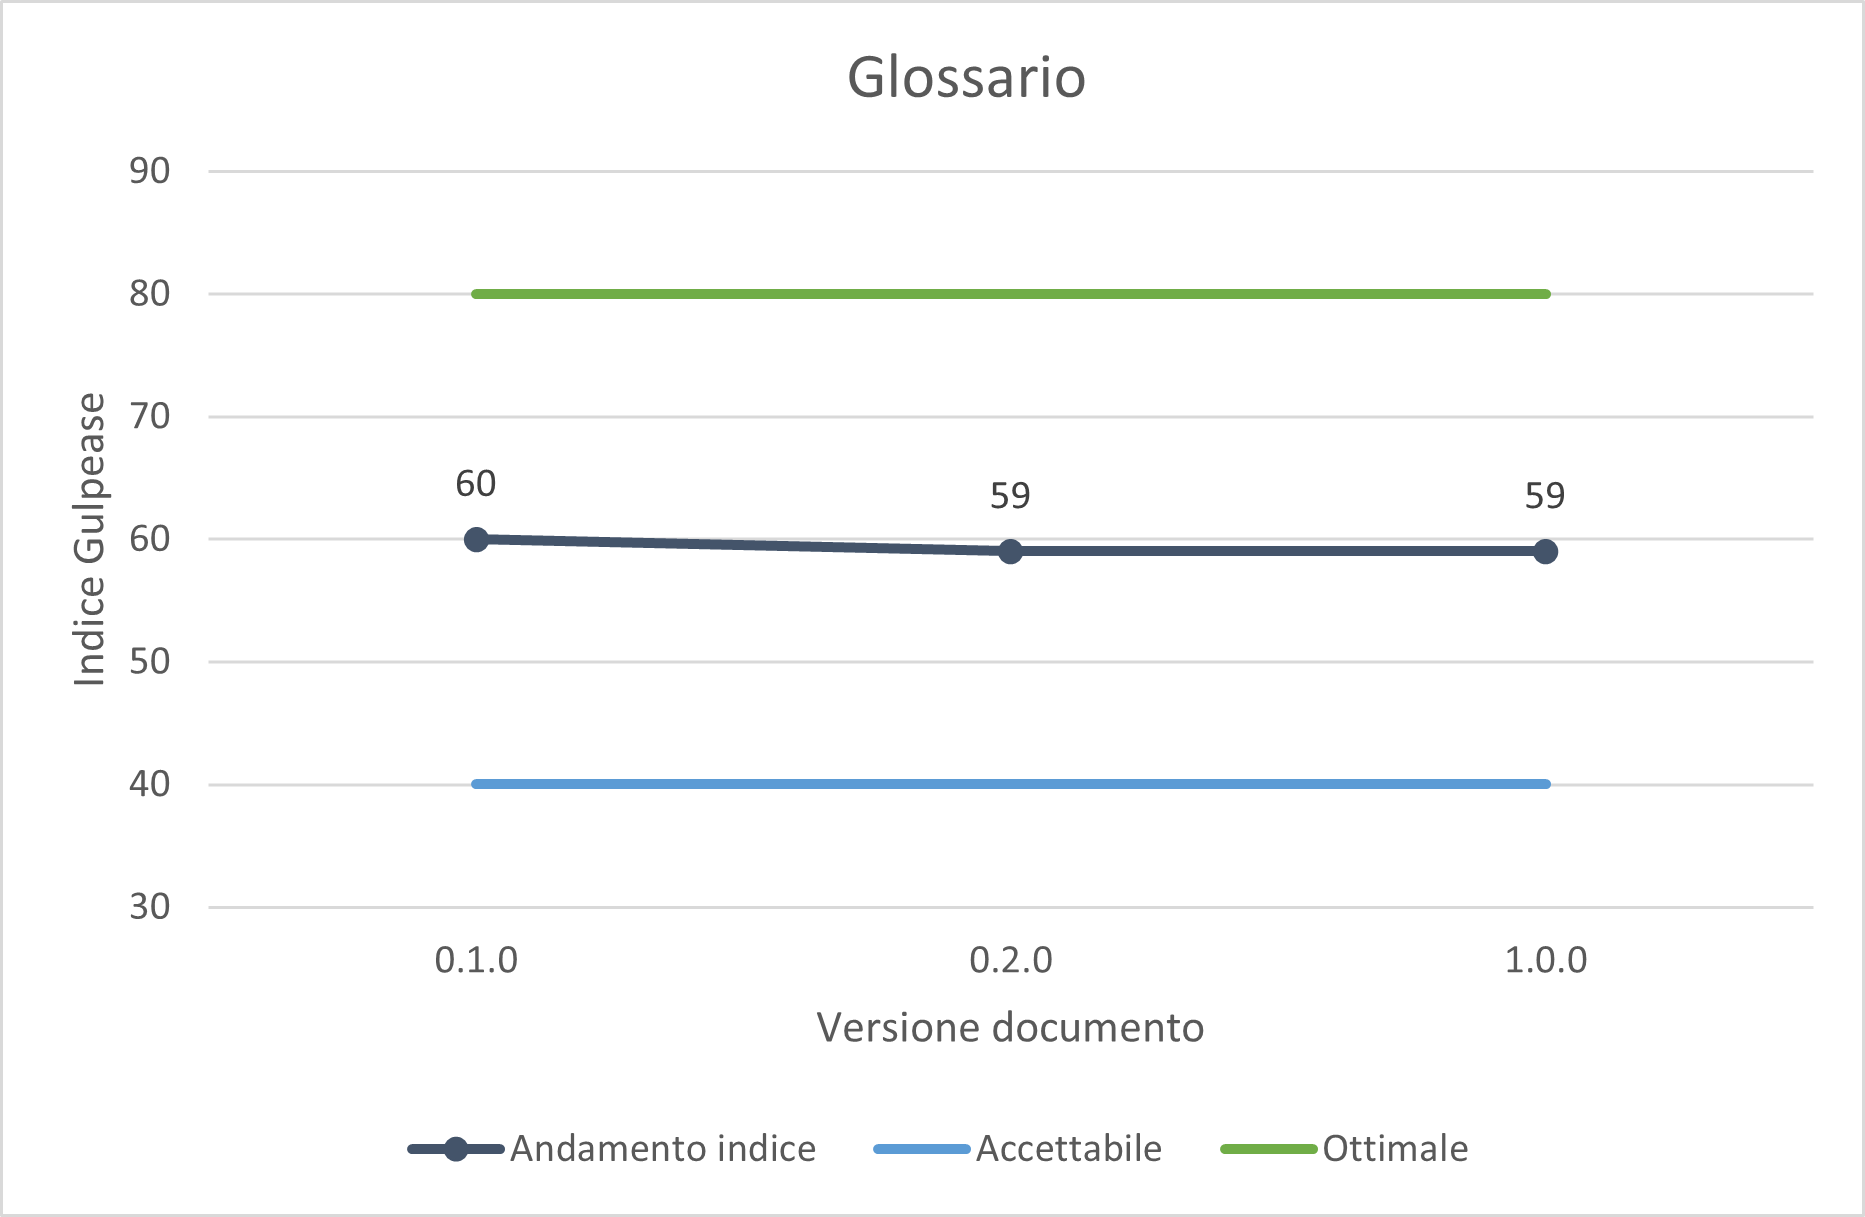
\includegraphics[scale=0.90]{res/ResocontoAttivitaDiVerifica/res/img/gulpeaseG.png}\\
\caption{Andamento dell'indice di Gulpease \Glossario}
\end{figure}



\subsubsection{MPC4 - Correttezza ortografica}
Di seguito è riportato il grafico degli errori ortografici rilevati sui vari documenti, il cui valore è definito accettabile e ottimale come descritto nella sezione §2.2.1.2.\\

\begin{figure}[H]
\centering
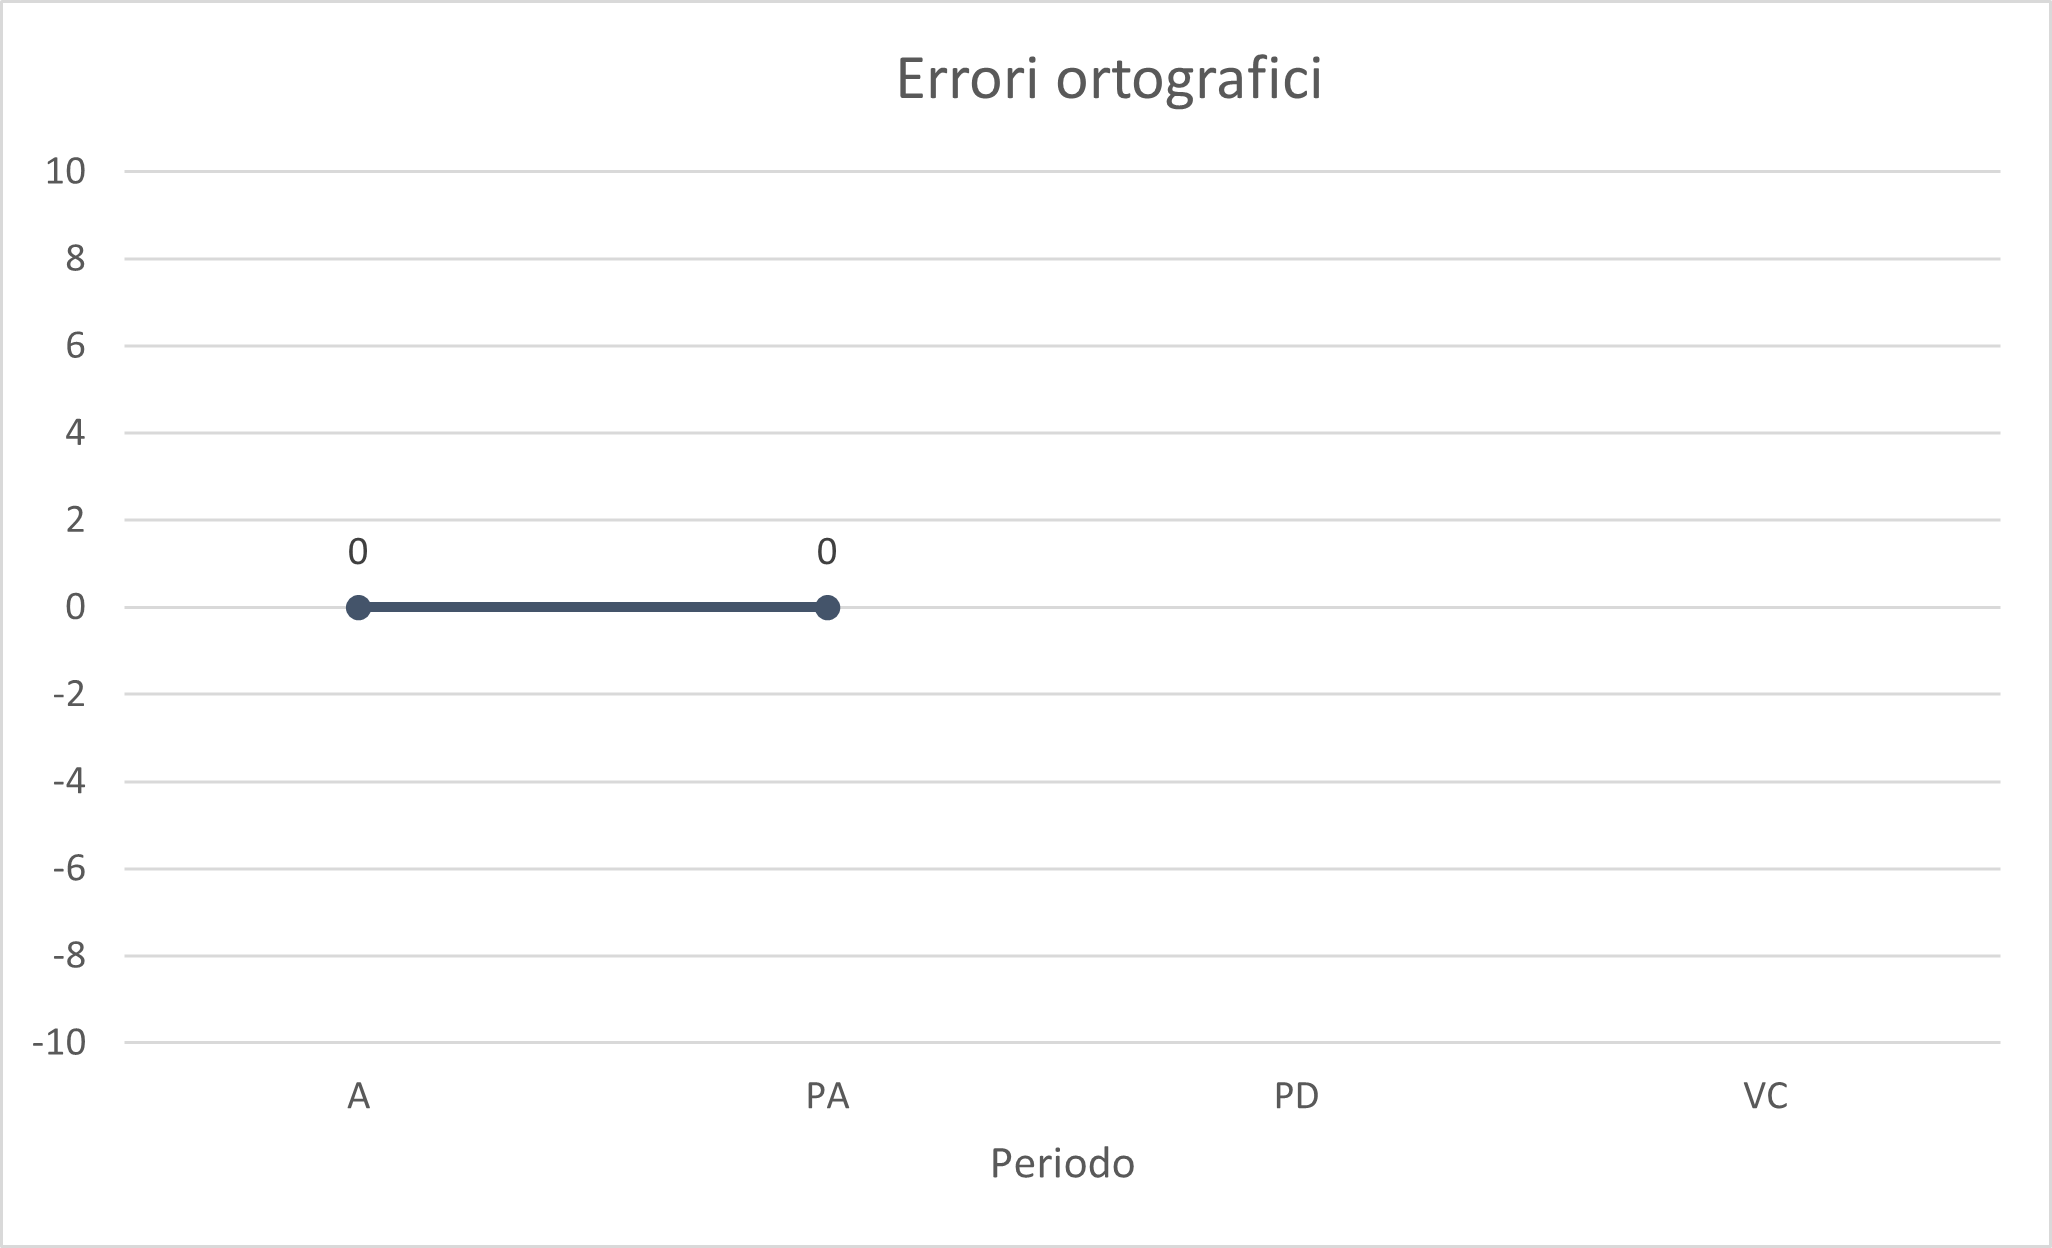
\includegraphics[scale=0.78]{res/ResocontoAttivitaDiVerifica/res/metriche/grafici/img/correttezzaOrtografica.png}\\
\caption{Andamento della correttezza ortografica}
\end{figure}

\subsubsection{MPC5 - Code Coverage}
Di seguito è riportato il grafico del Code Coverage relativo al modulo Front-end{G} e Back-end\ped{G}, i cui valori sono definiti accettabili e ottimali come descritto nella sezione §2.2.2.1.\\

\begin{figure}[H]
\centering
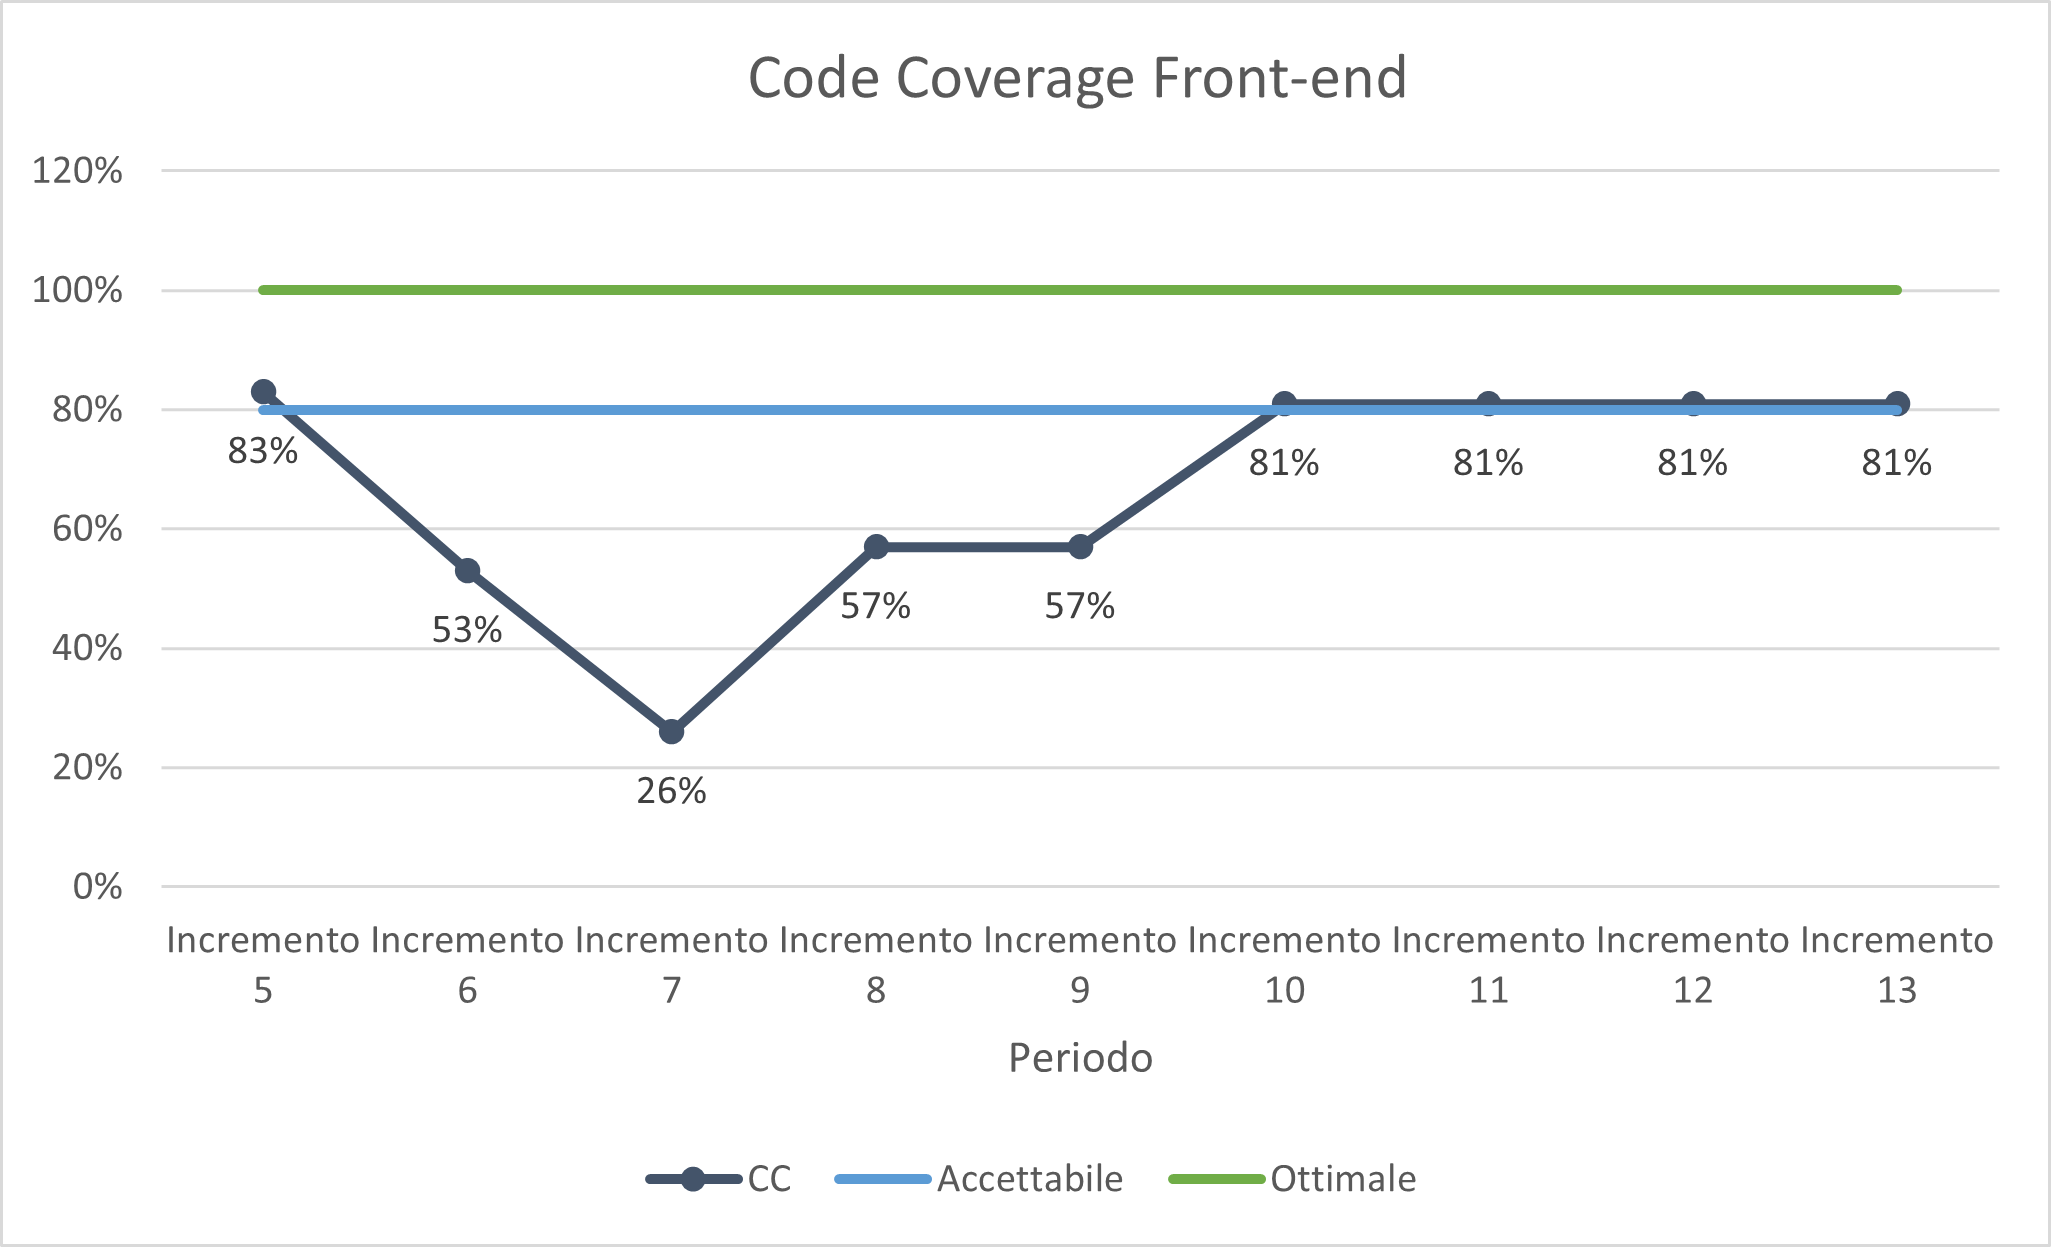
\includegraphics[scale=0.78]{res/ResocontoAttivitaDiVerifica/res/metriche/grafici/img/CCFE.png}\\
\caption{Andamento percentuale Code Coverage Front-end}
\end{figure}

\begin{figure}[H]
\centering
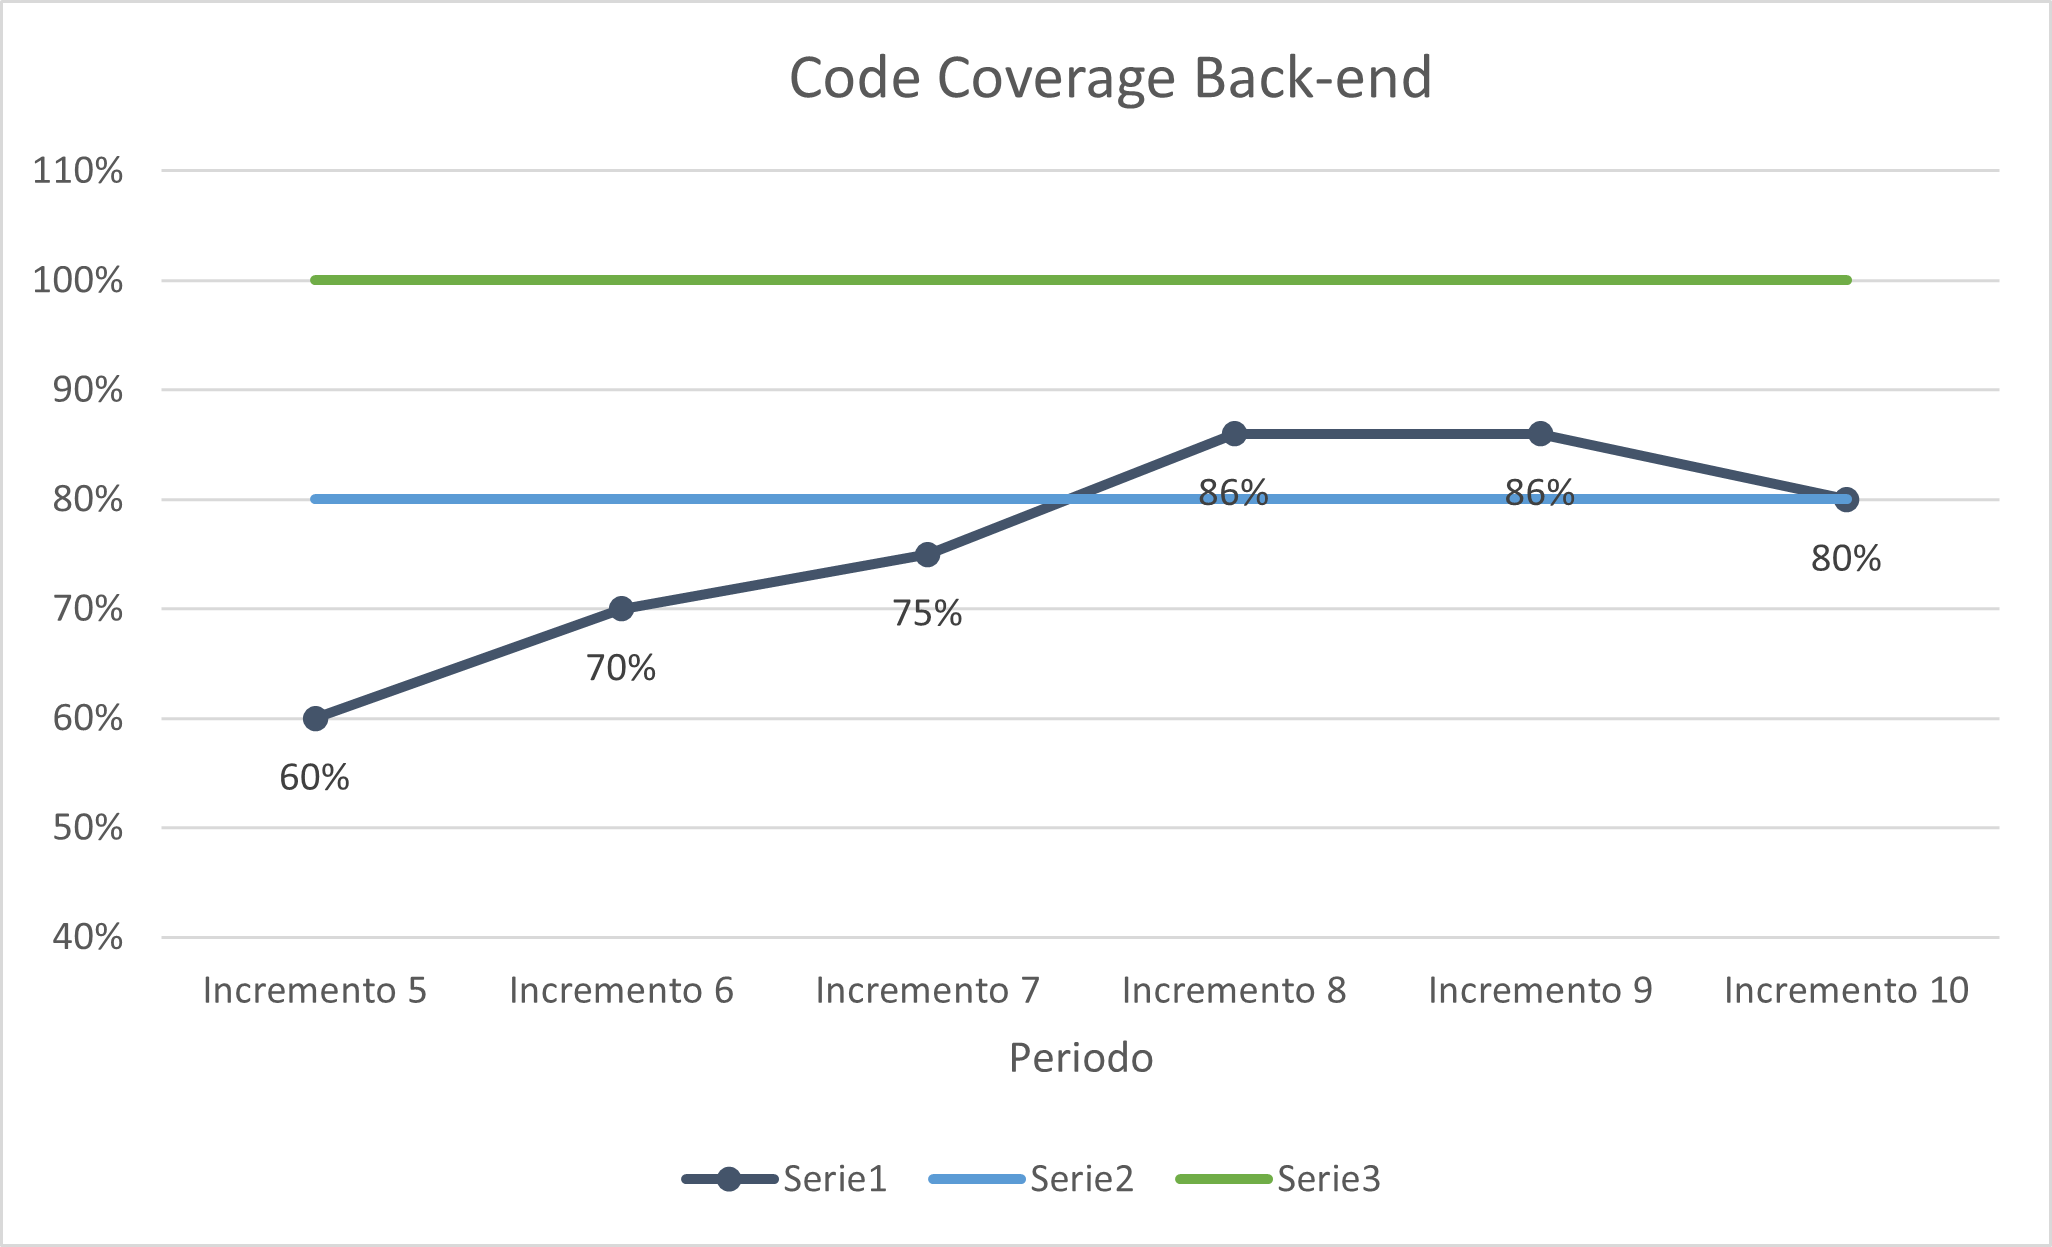
\includegraphics[scale=0.78]{res/ResocontoAttivitaDiVerifica/res/metriche/grafici/img/CCBE.png}\\
\caption{Andamento percentuale Code Coverage Back-end}
\end{figure}

\subsubsection{MPC6 - Estimate at Completion}
Di seguito è riportato il grafico dell'Estimate at Completion, il cui valore è definito accettabile e ottimale come descritto nella sezione §2.3.1.1.\\

\begin{figure}[H]
\centering
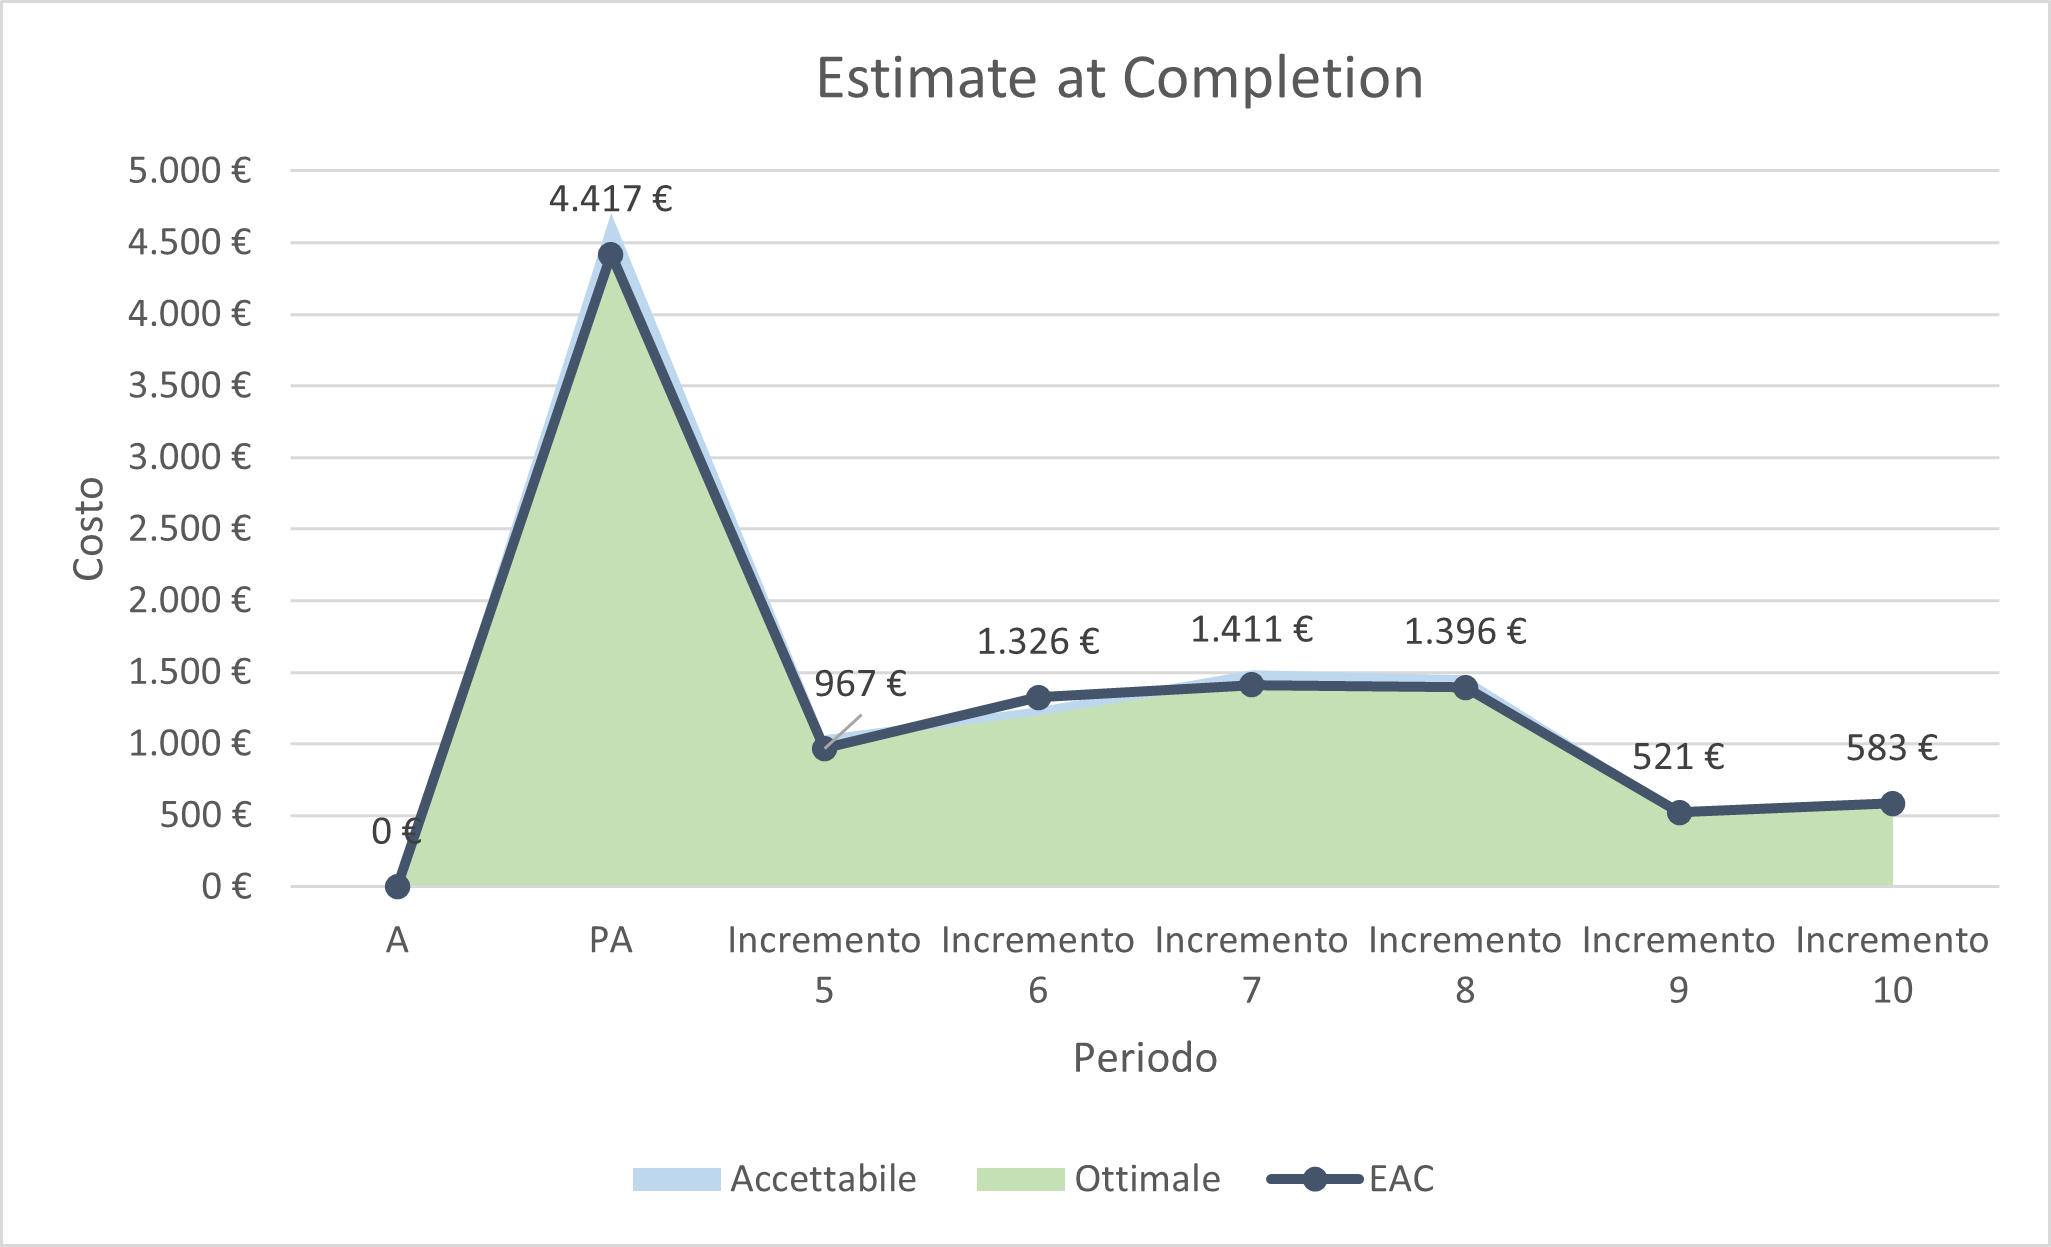
\includegraphics[scale=0.78]{res/ResocontoAttivitaDiVerifica/res/metriche/grafici/img/estimateCompletion.png}\\
\caption{Andamento Estimate at Completion}
\end{figure}

\subsubsection{MPC7 - Variance at Completion}
Di seguito è riportato il grafico della Variance at Completion, il cui valore è definito accettabile e ottimale come descritto nella sezione §2.3.1.2.\\

\begin{figure}[H]
\centering
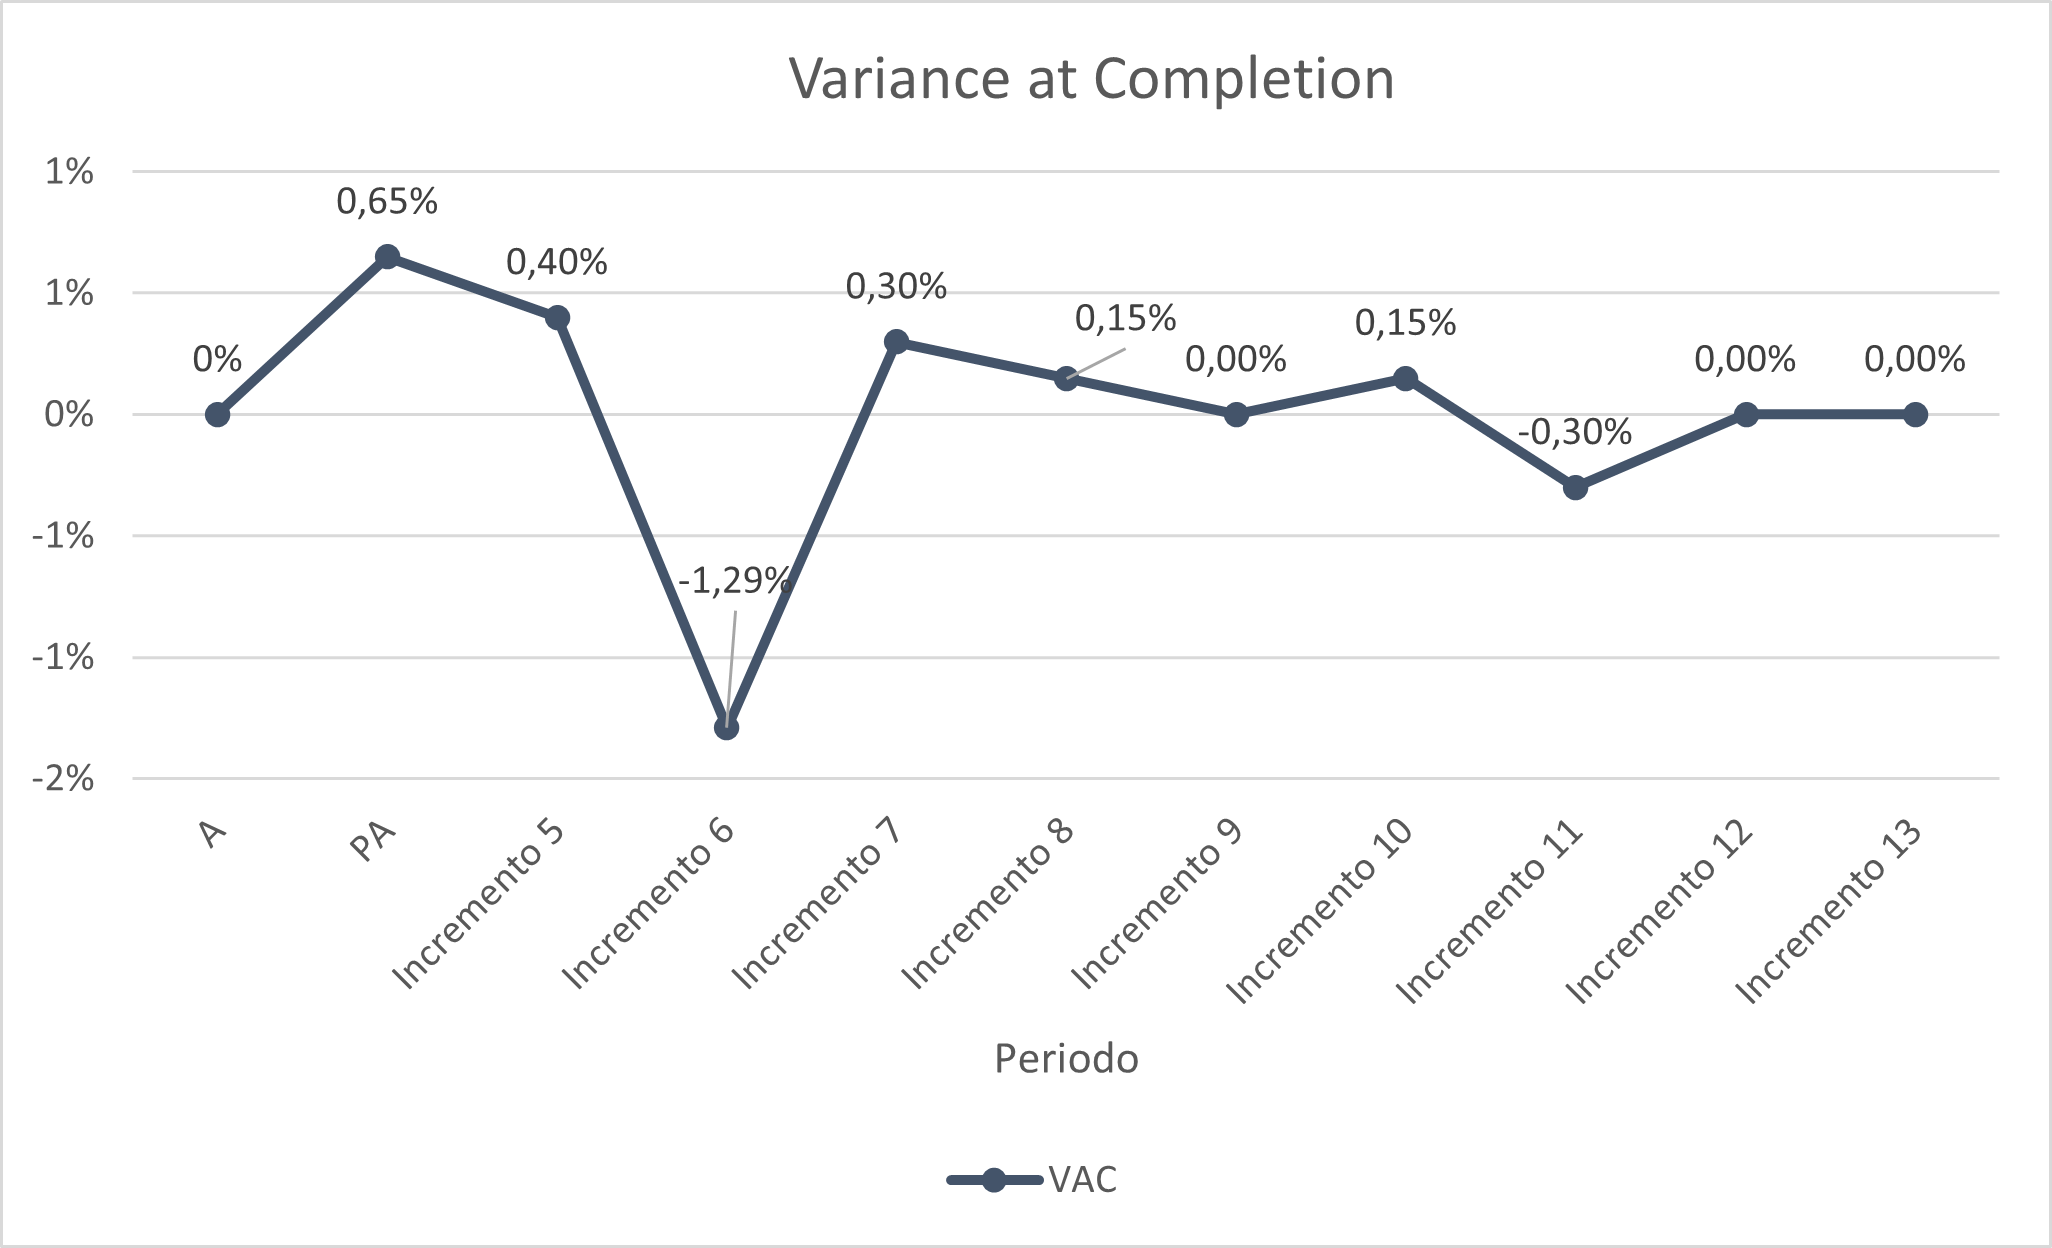
\includegraphics[scale=0.78]{res/ResocontoAttivitaDiVerifica/res/metriche/grafici/img/varianceCompletion.png}\\
\caption{Andamento Variance at Completion}
\end{figure}

\subsubsection{MPC8 - Actual Cost}
Di seguito è riportato il grafico dell'Actual Cost, il cui valore è definito accettabile e ottimale come descritto nella sezione §2.3.1.3.\\

\begin{figure}[H]
\centering
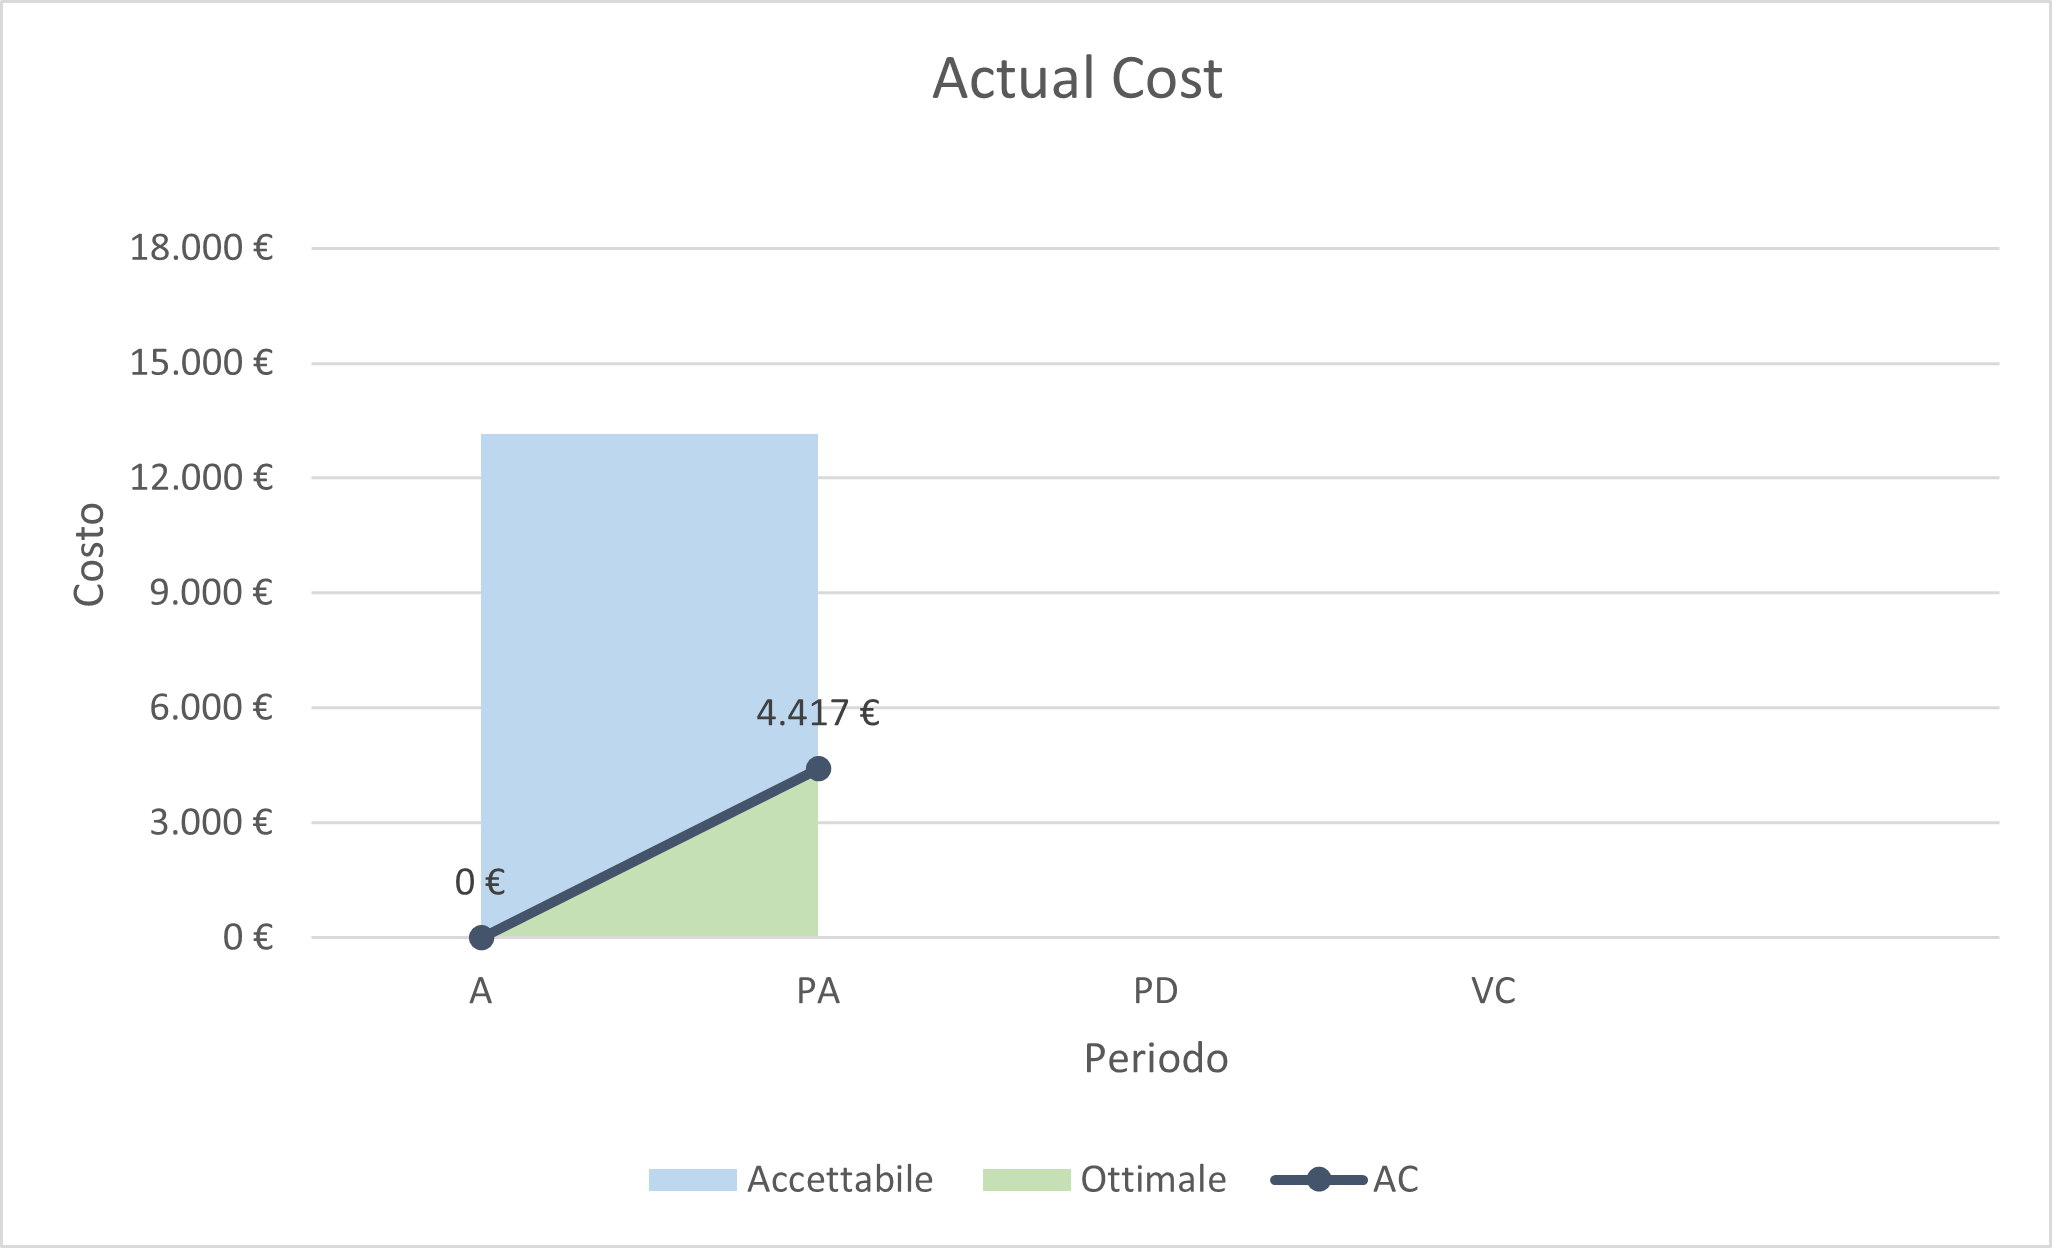
\includegraphics[scale=0.78]{res/ResocontoAttivitaDiVerifica/res/metriche/grafici/img/actualCost.png}\\
\caption{Andamento Actual Cost}
\end{figure}

\subsubsection{MPC9 - Schedule Variance}
Di seguito è riportato il grafico dello Schedule Variance, il cui valore è definito accettabile e ottimale come descritto nella sezione §2.3.1.4.\\

\begin{figure}[H]
\centering
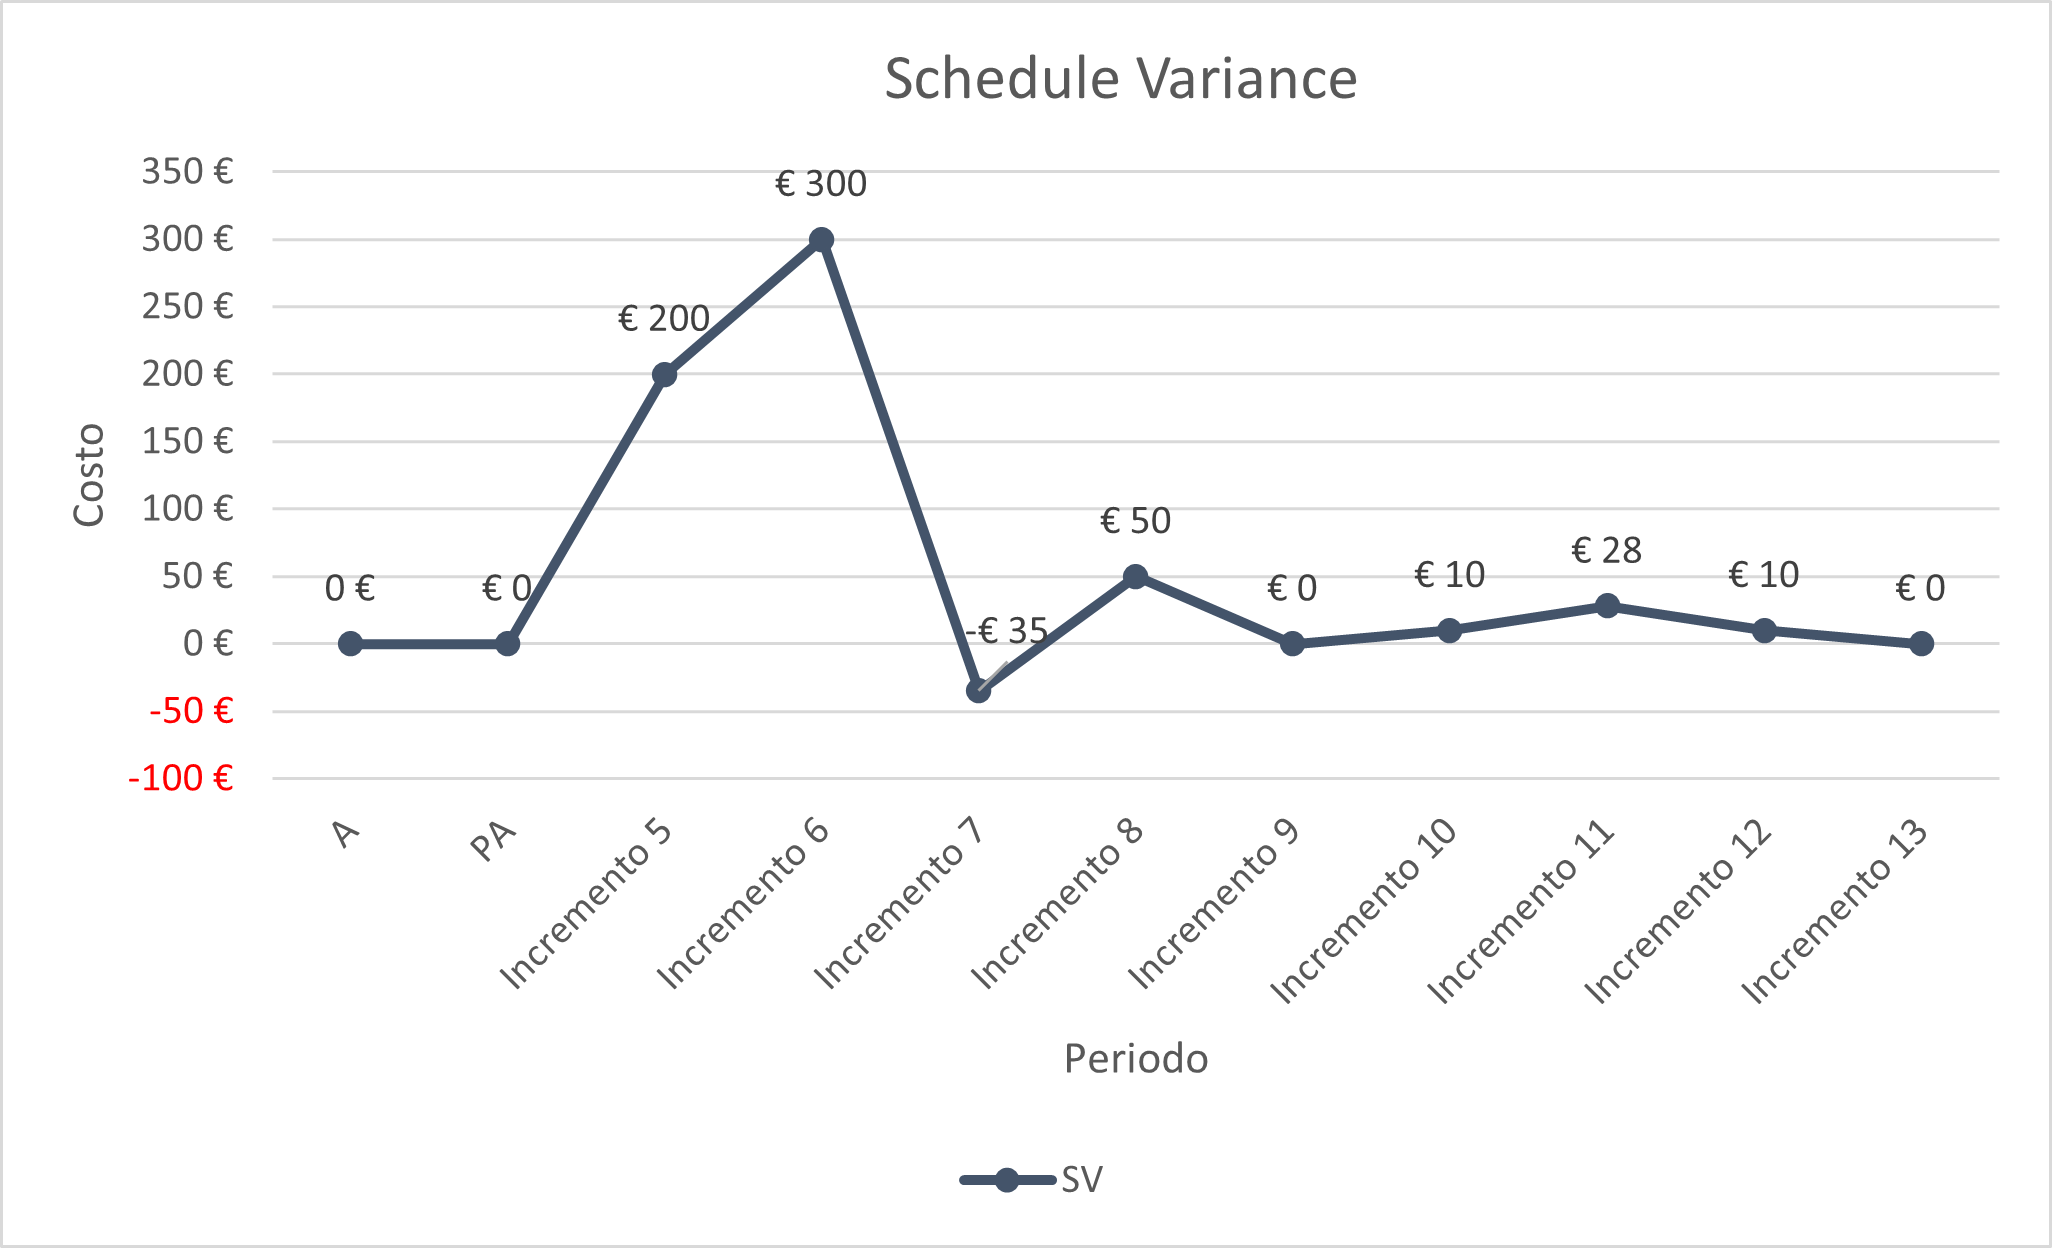
\includegraphics[scale=0.78]{res/ResocontoAttivitaDiVerifica/res/metriche/grafici/img/scheduleVariance.png}\\
\caption{Andamento Schedule Variance}
\end{figure}

\subsubsection{MPC10 - Budget Variance}
Di seguito è riportato il grafico del Budget Variance, il cui valore è definito accettabile e ottimale come descritto nella sezione §2.3.1.5.\\

\begin{figure}[H]
\centering
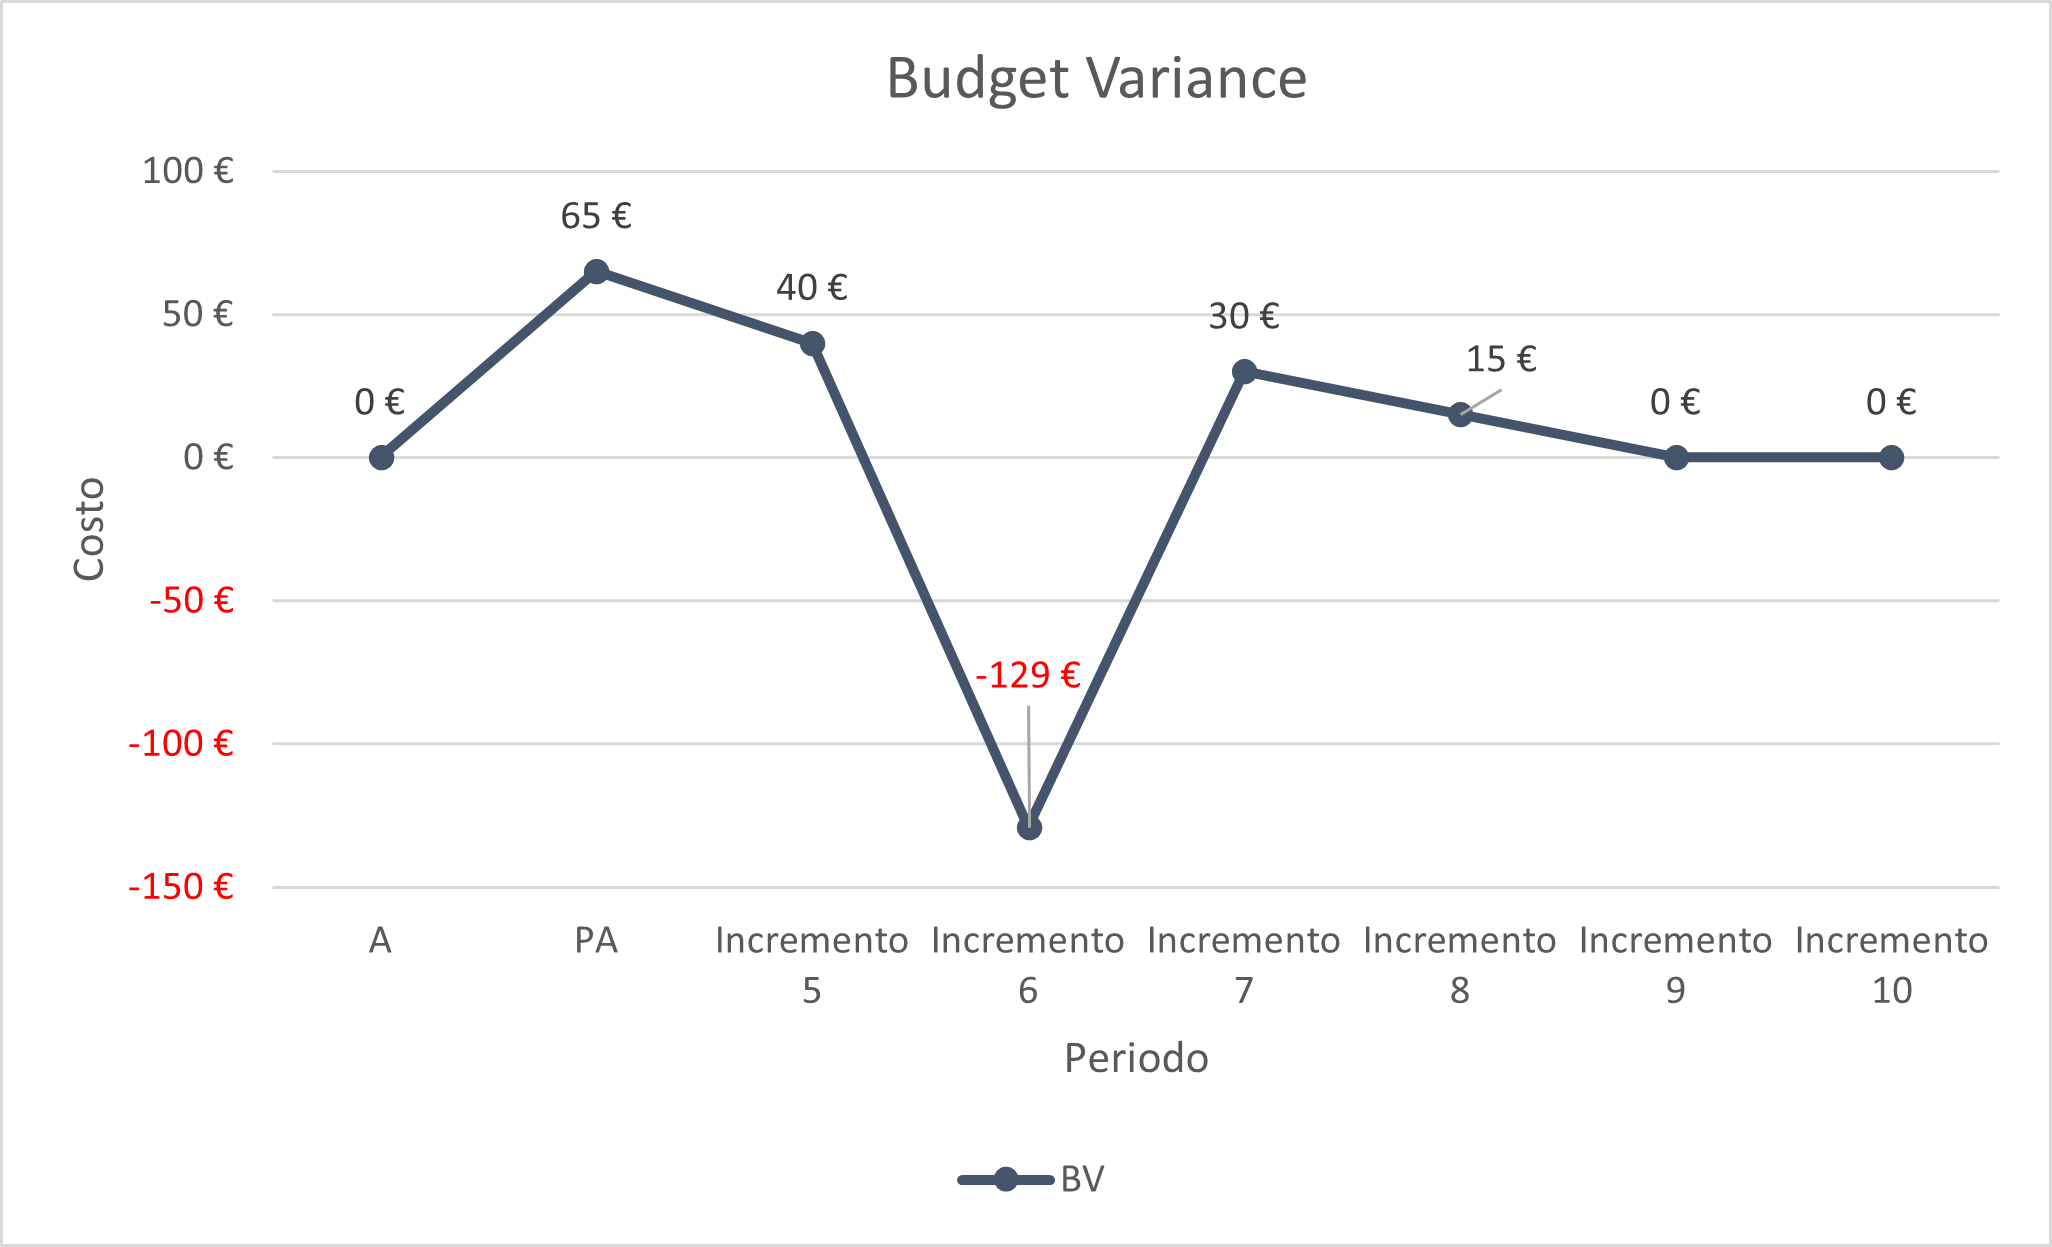
\includegraphics[scale=0.78]{res/ResocontoAttivitaDiVerifica/res/metriche/grafici/img/budgetVariance.png}\\
\caption{Andamento Budget Variance}
\end{figure}


\subsubsection{MPC11 - Percentuale di metriche soddisfatte}
Di seguito è riportato il grafico della percentuale di metriche soddisfatte, il cui valore è definito accettabile e ottimale come descritto nella sezione §2.3.1.6.\\

\begin{figure}[H]
\centering
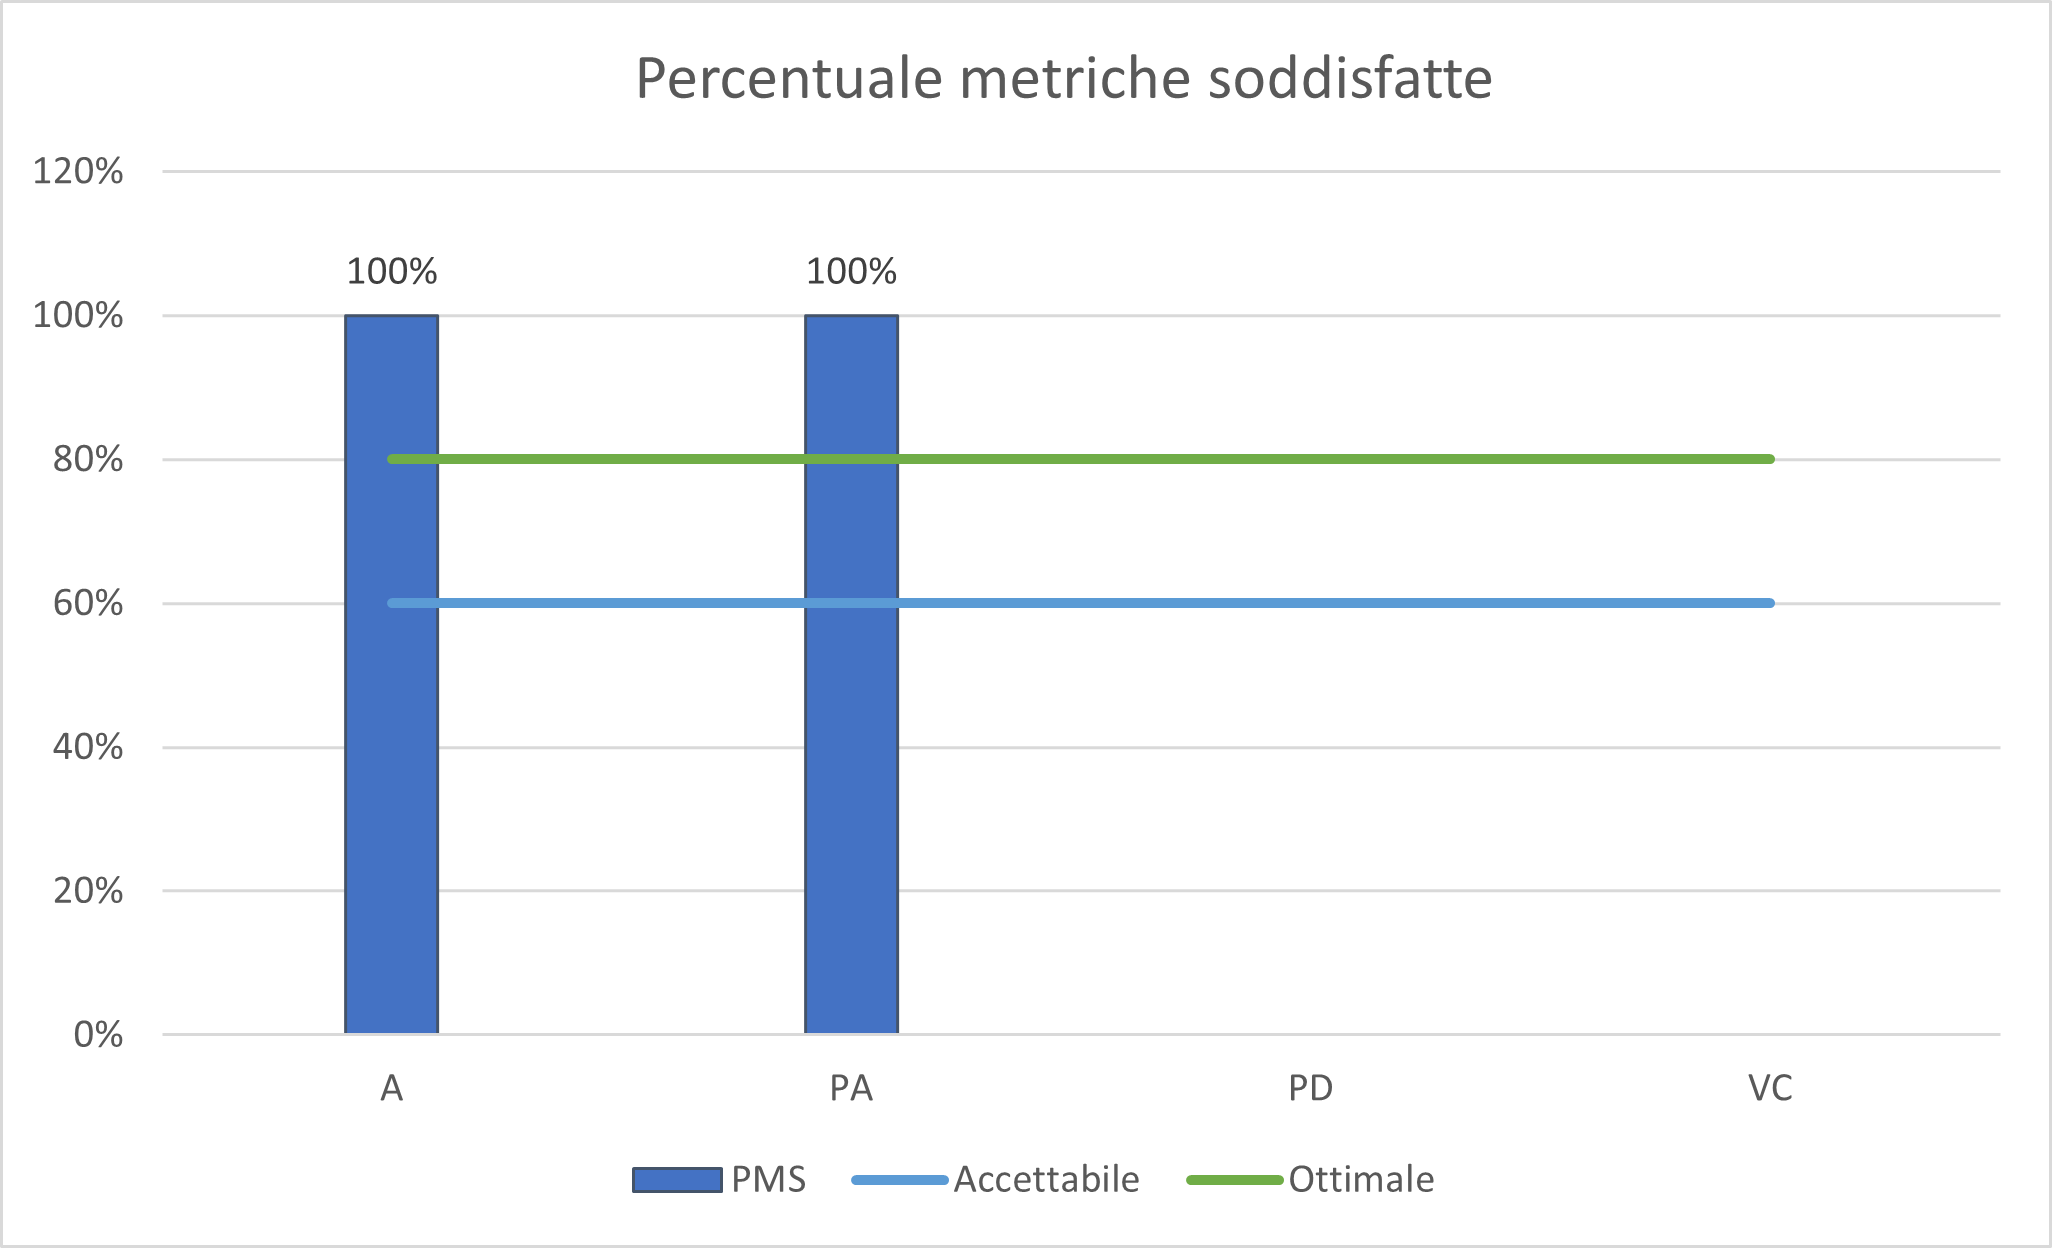
\includegraphics[scale=0.78]{res/ResocontoAttivitaDiVerifica/res/metriche/grafici/img/metricheSoddisfatte.png}\\
\caption{Andamento percentuale delle metriche soddisfatte}
\end{figure}


\subsubsection{MPD1 - Completezza informazioni}
Di seguito è riportato il grafico della completezza delle informazioni, il cui valore è definito accettabile e ottimale come descritto nella sezione §3.1.2.1.\\

\begin{figure}[H]
\centering
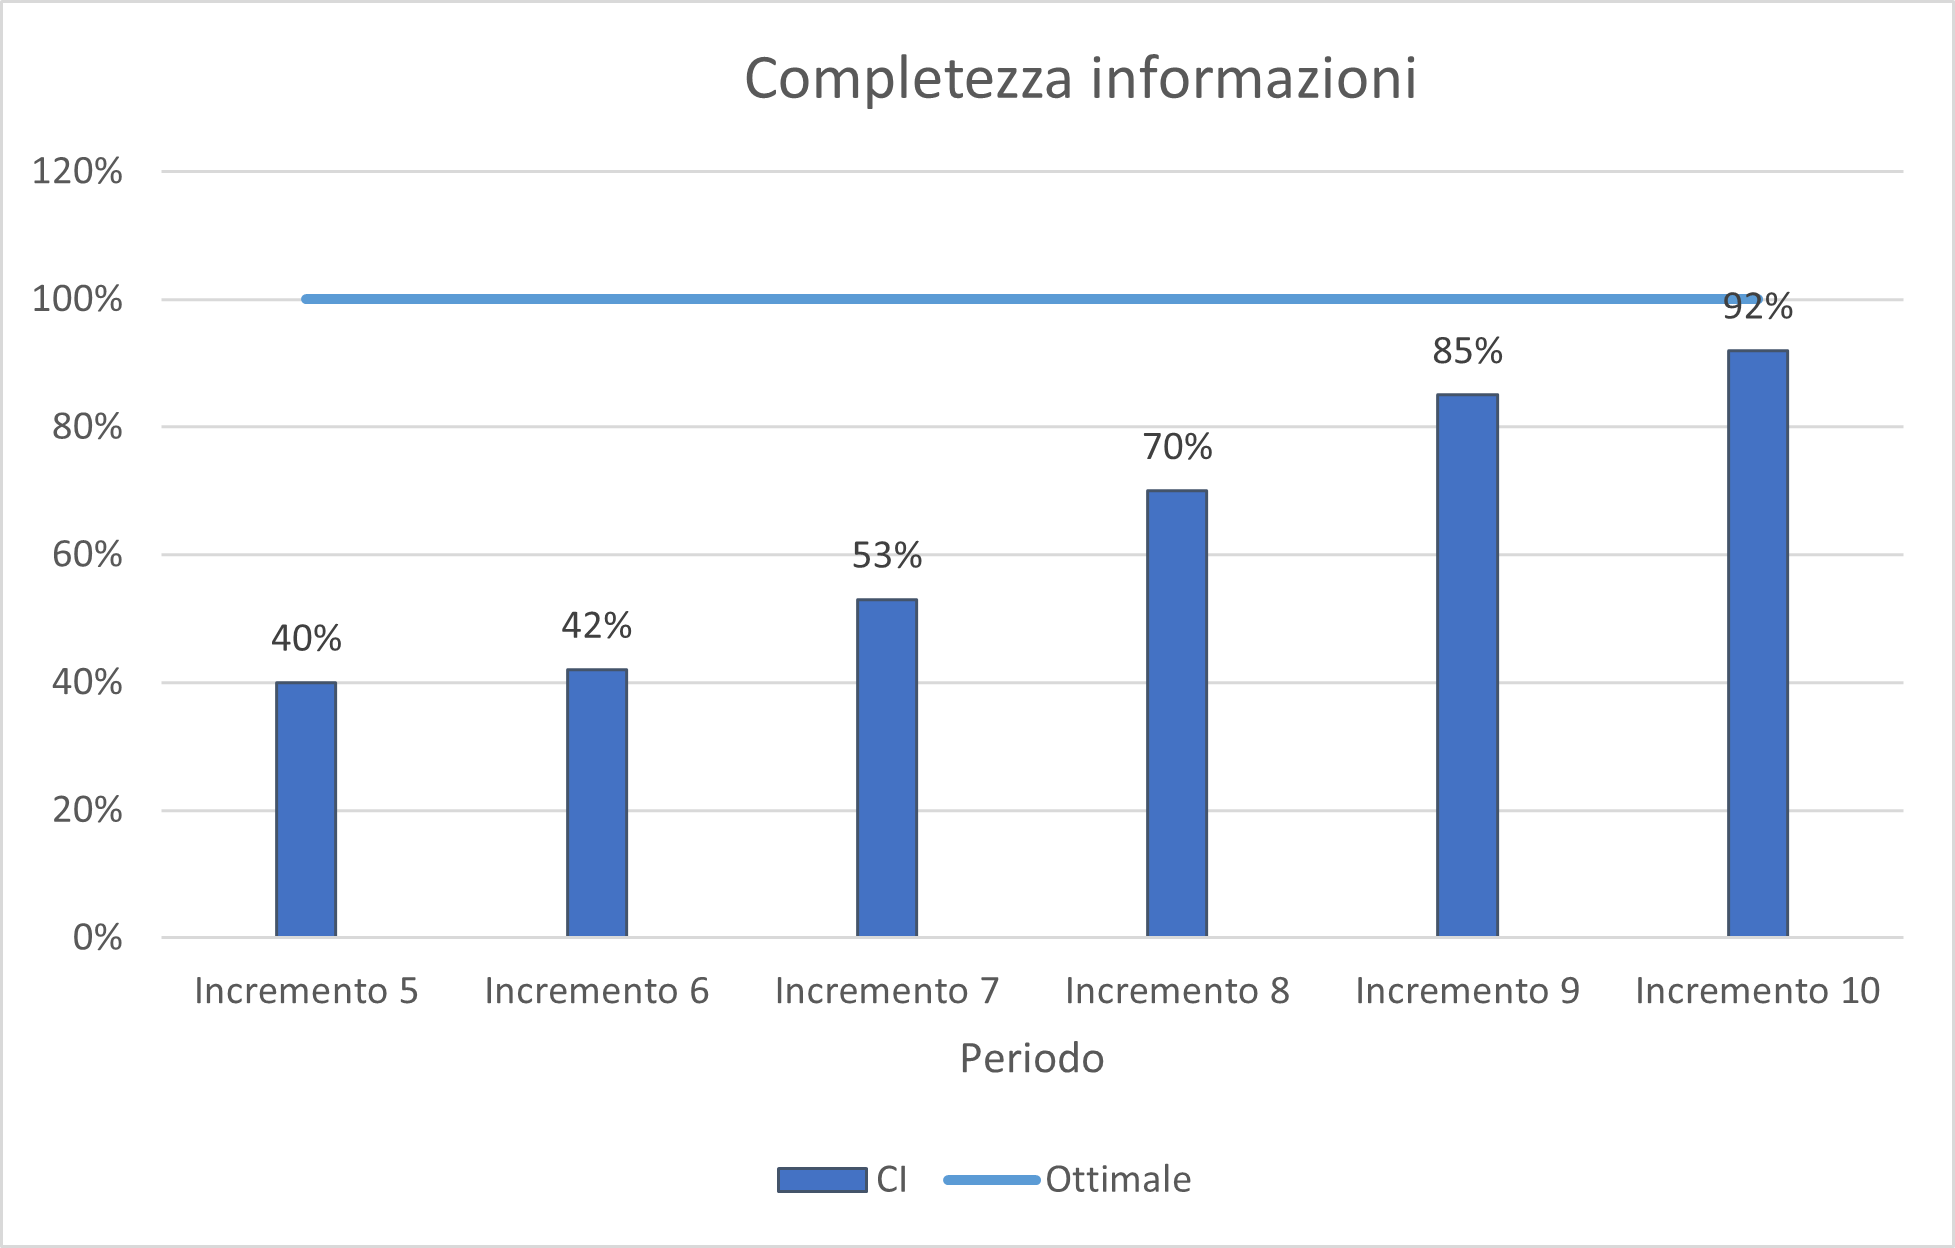
\includegraphics[scale=0.78]{res/ResocontoAttivitaDiVerifica/res/metriche/grafici/img/CompletezzaInformazioni.png}\\
\caption{Andamento percentuale completezza delle informazioni}
\end{figure}


\subsubsection{MPD2 - Densità degli errori}
Di seguito è riportato il grafico della densità degli errori, il cui valore è definito accettabile e ottimale come descritto nella sezione §3.2.2.1.\\

\begin{figure}[H]
\centering
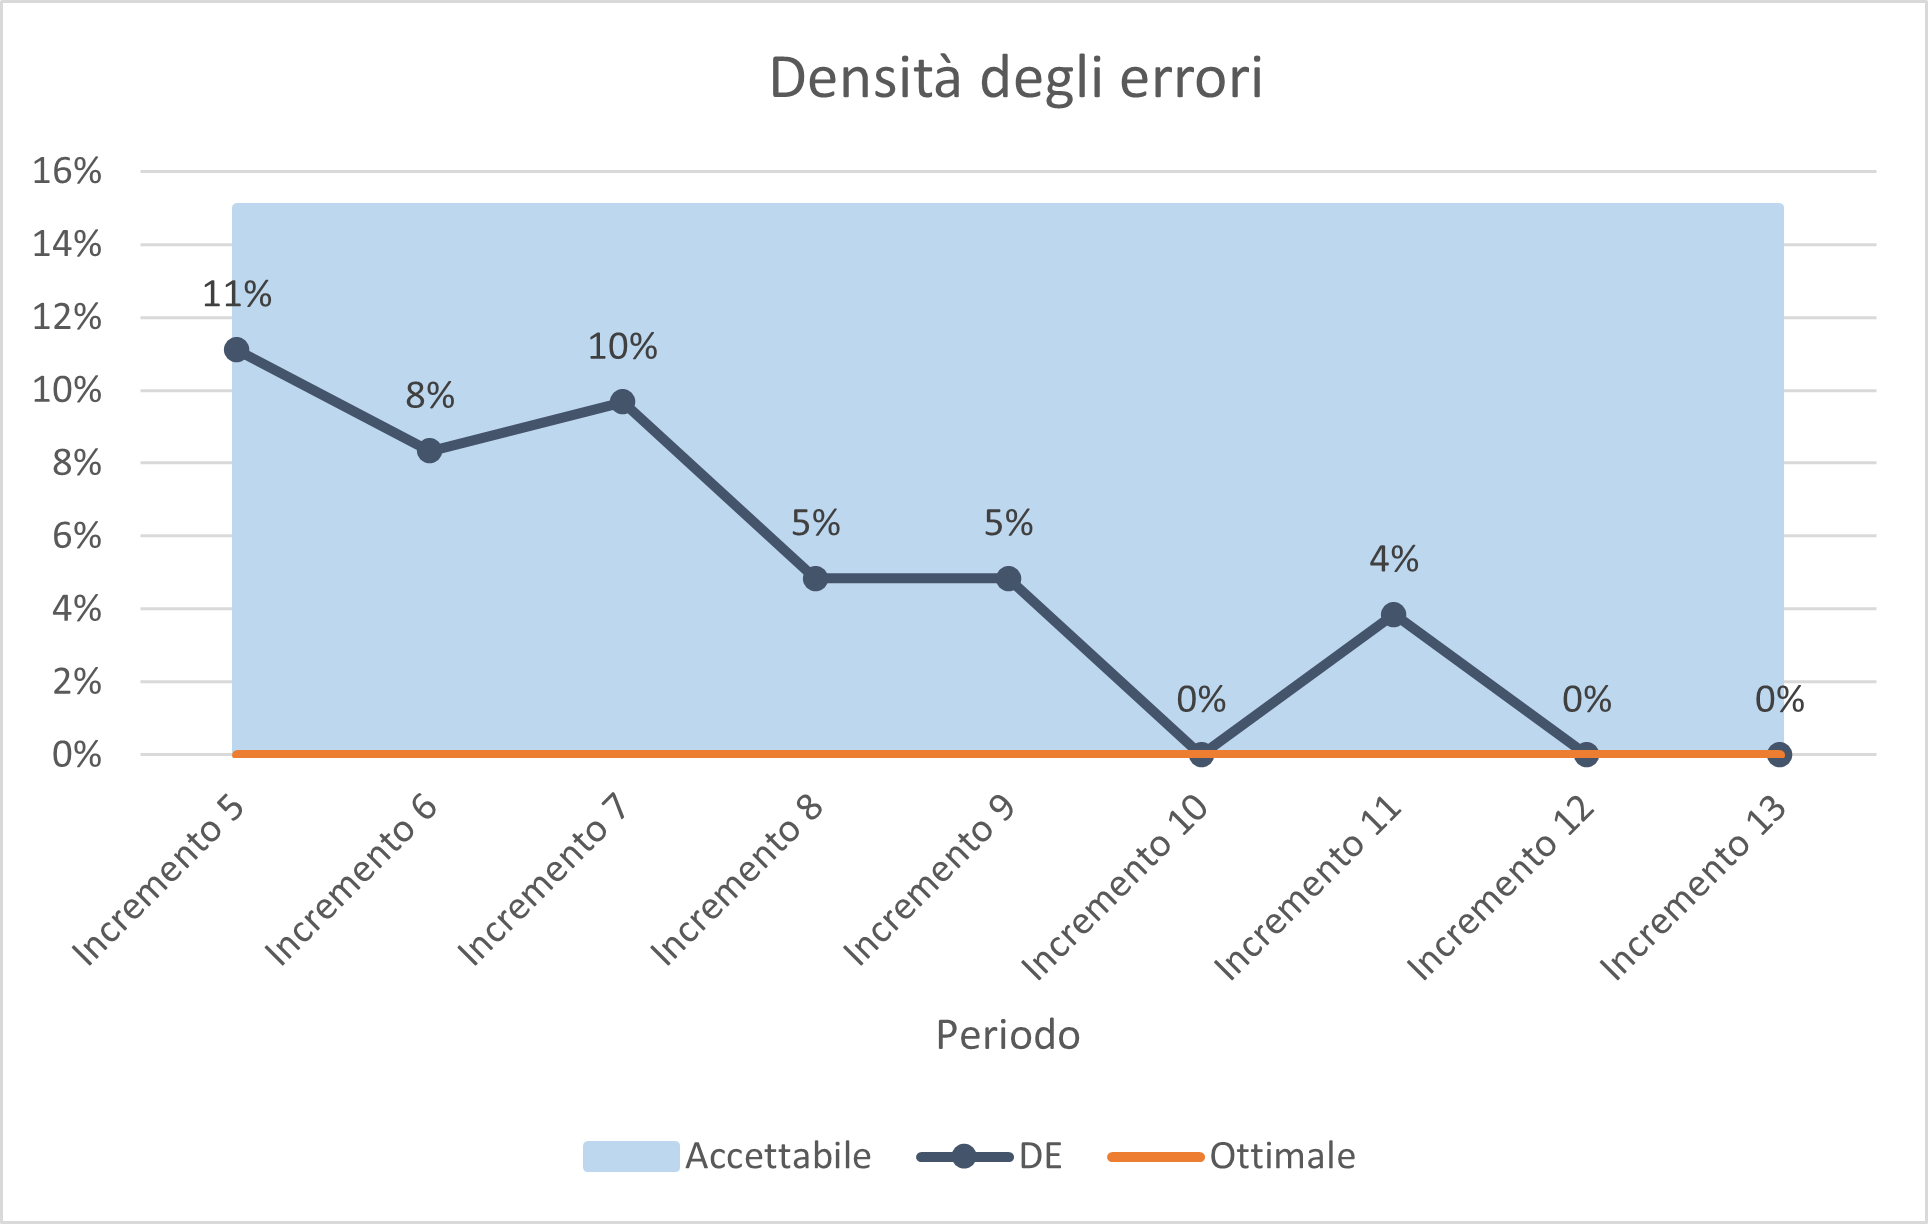
\includegraphics[scale=0.78]{res/ResocontoAttivitaDiVerifica/res/metriche/grafici/img/DensitaErrori.png}\\
\caption{Andamento percentuale densità degli errori}
\end{figure}

\subsubsection{MPD3 - Facilità di utilizzo}
Di seguito è riportato il grafico della facilità di utilizzo, il cui valore è definito accettabile e ottimale come descritto nella sezione §3.3.2.1.\\

\begin{figure}[H]
\centering
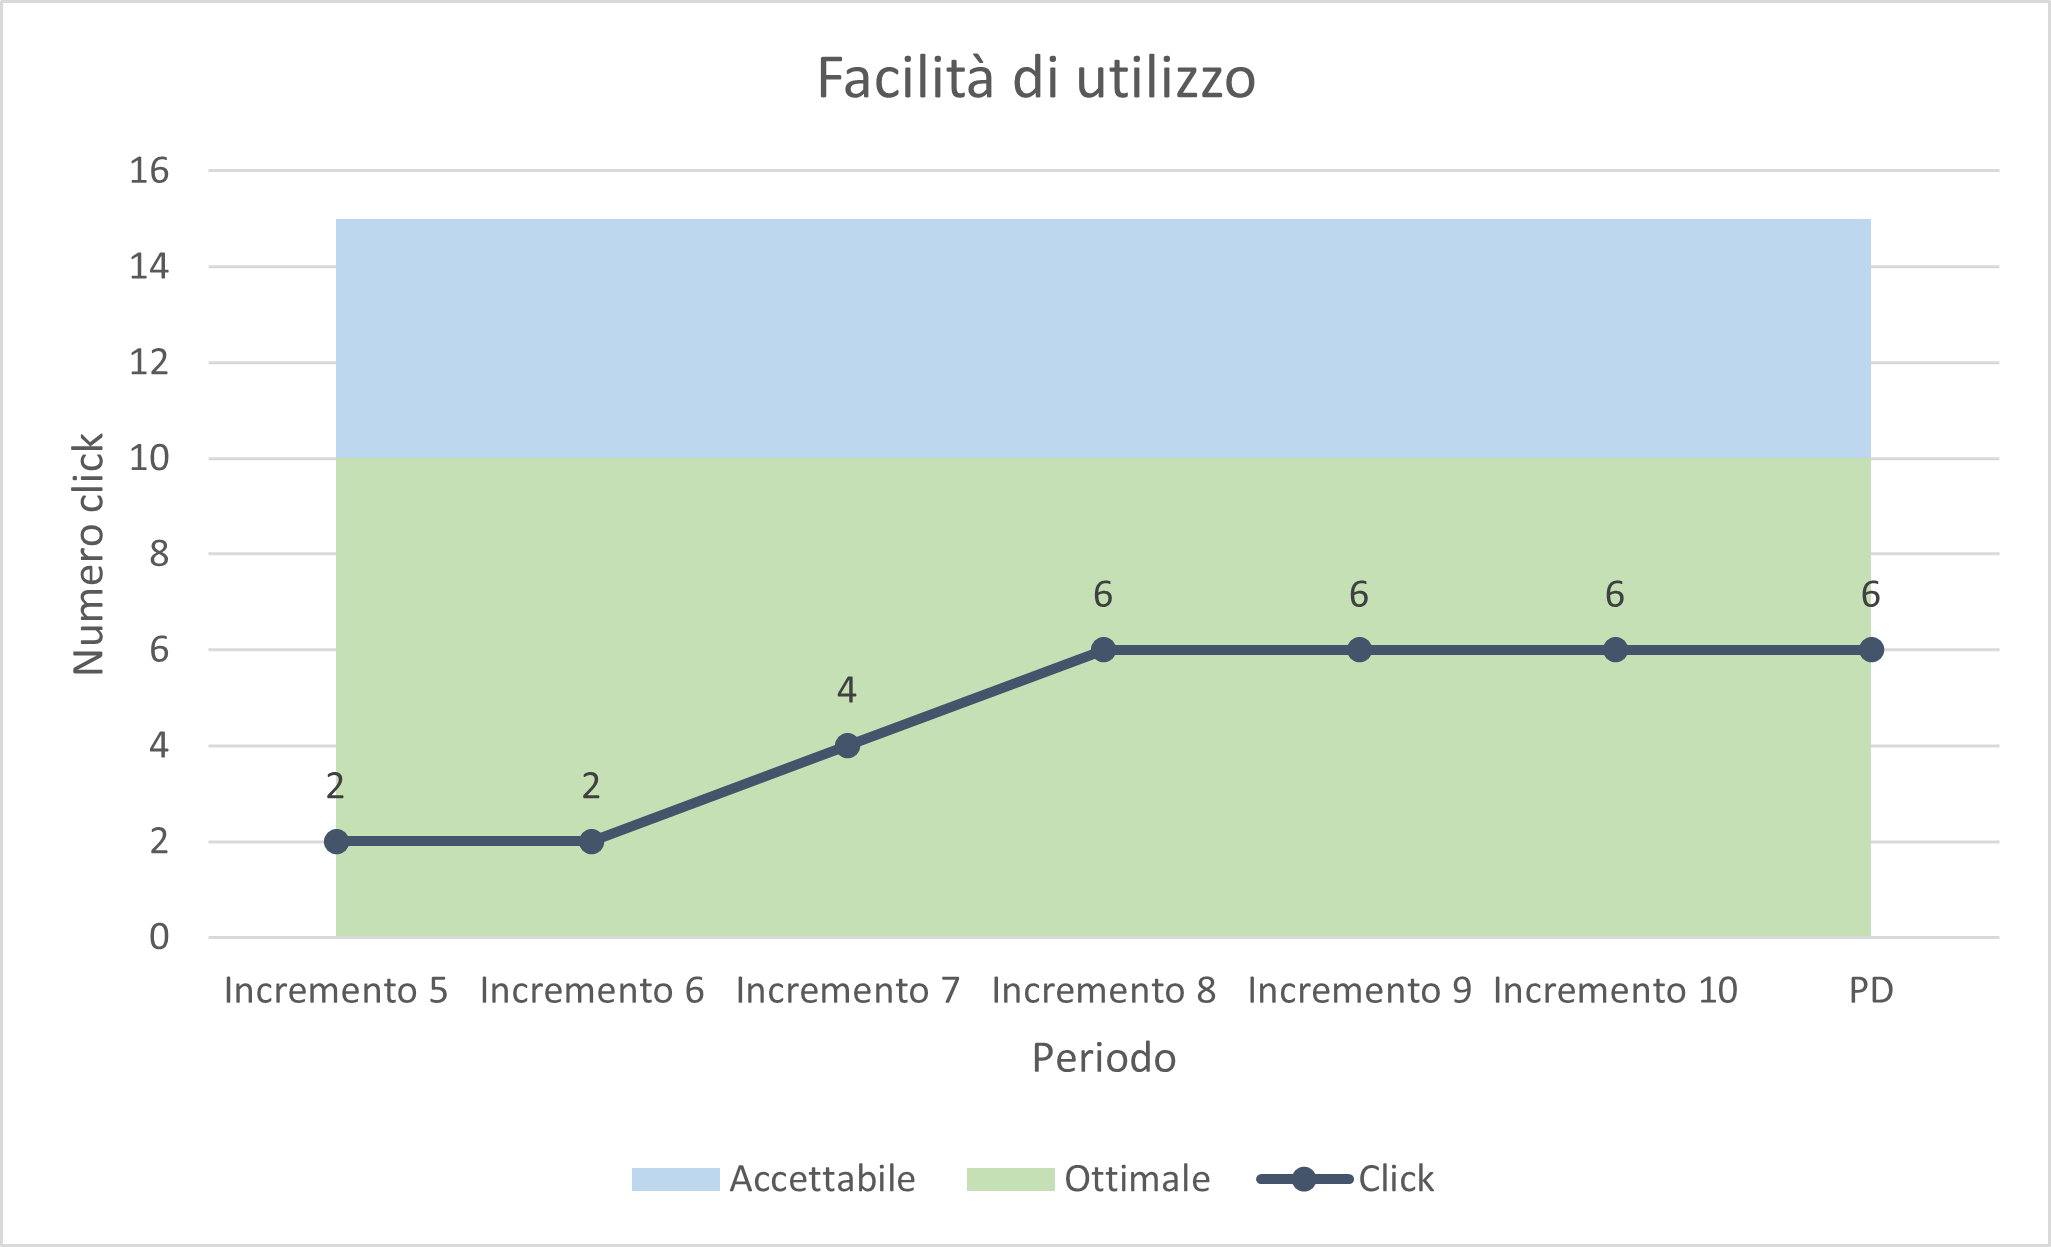
\includegraphics[scale=0.78]{res/ResocontoAttivitaDiVerifica/res/metriche/grafici/img/FacilitaUtilizzo.png}\\
\caption{Andamento facilità di utilizzo}
\end{figure}

\subsubsection{MPD4 - Facilità di apprendimento}
Di seguito è riportato il grafico della facilità di apprendimento, il cui valore è definito accettabile e ottimale come descritto nella sezione §3.3.2.2.\\

\begin{figure}[H]
\centering
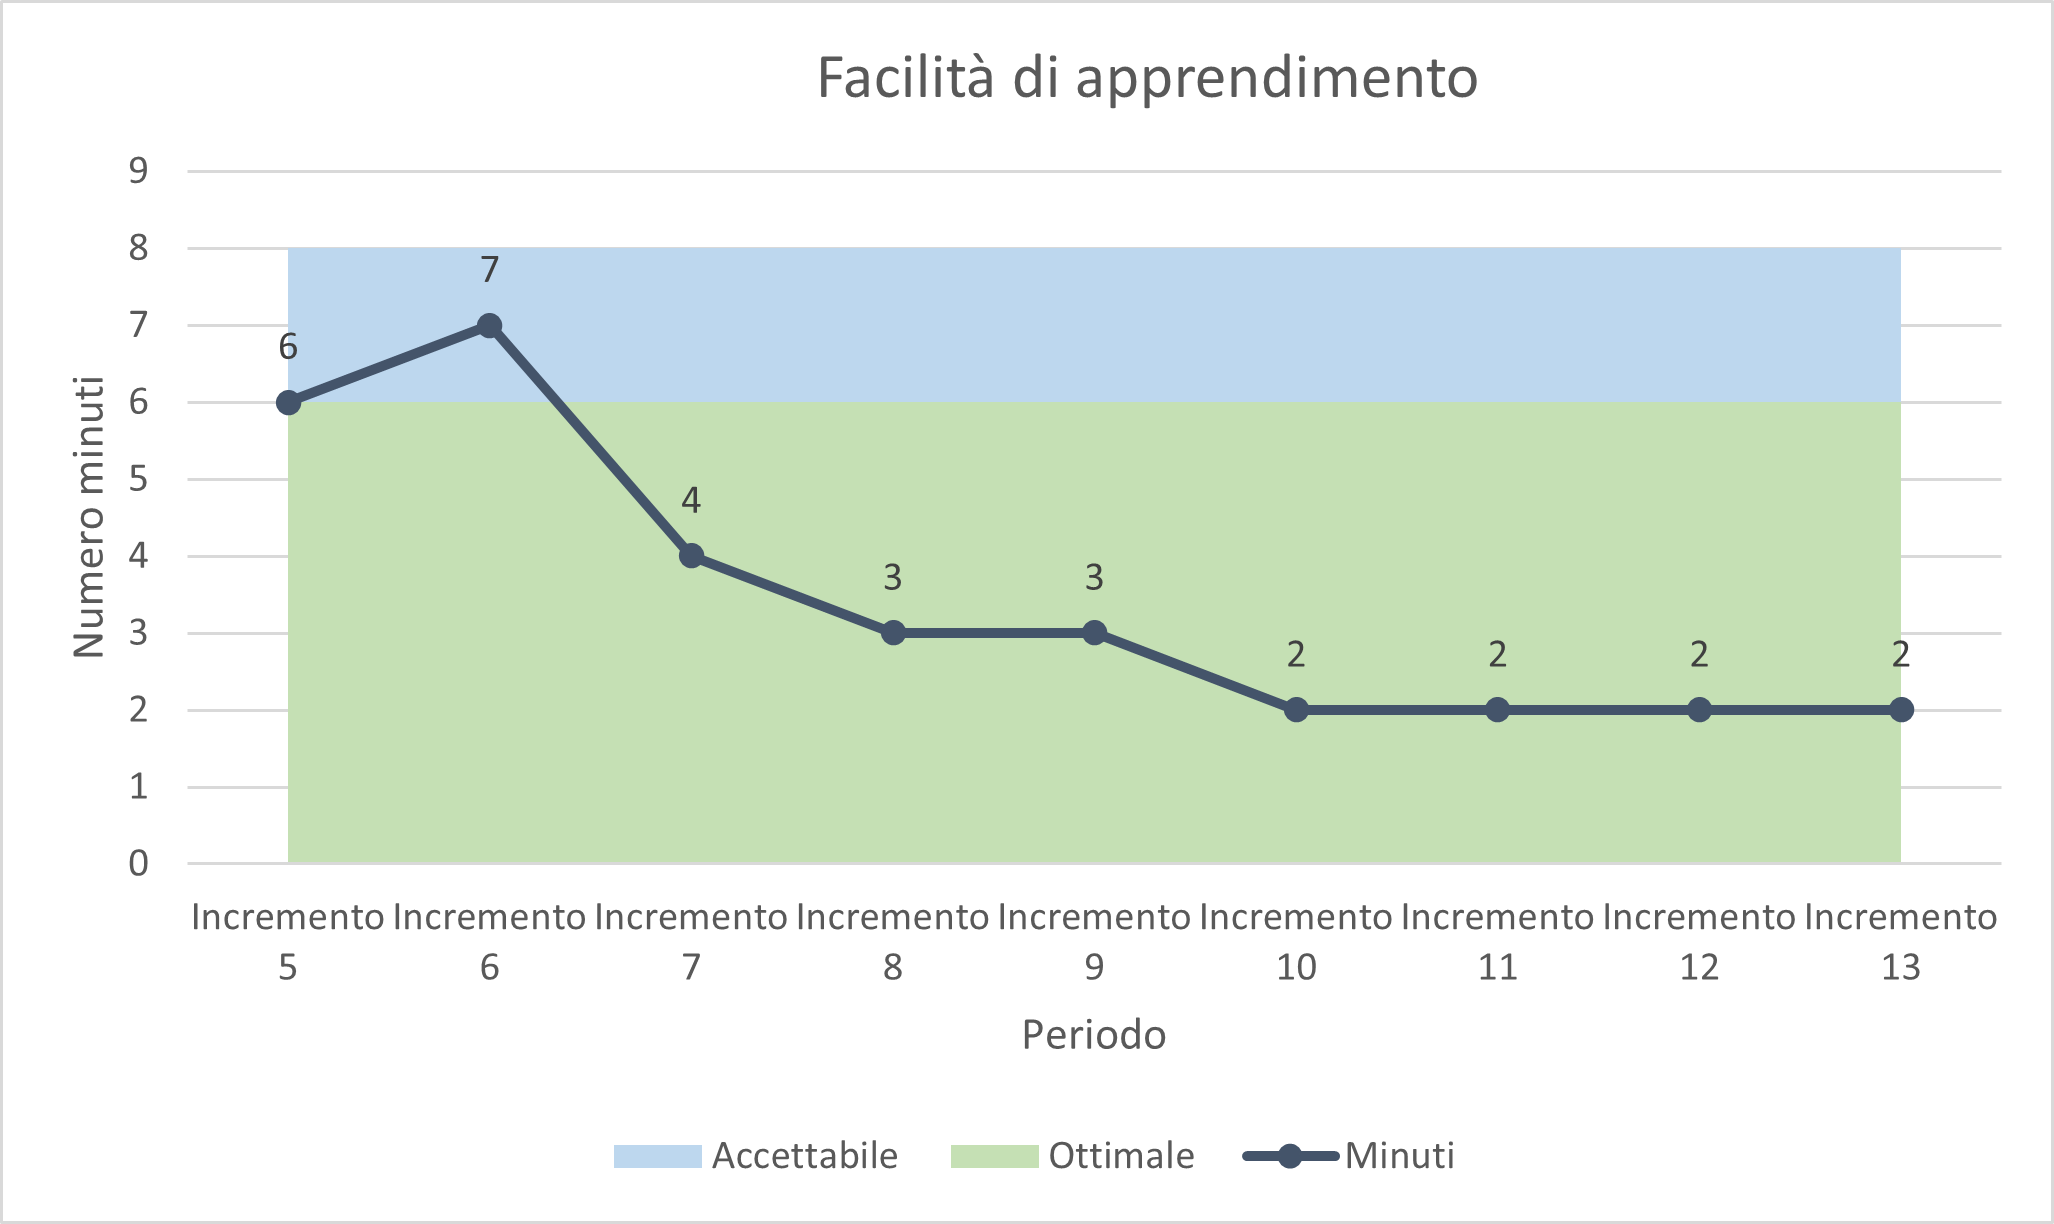
\includegraphics[scale=0.78]{res/ResocontoAttivitaDiVerifica/res/metriche/grafici/img/FacilitaApprendimento.png}\\
\caption{Andamento facilità di apprendimento}
\end{figure}

\subsubsection{MPD5 - Dimensione gerarchia}
Di seguito sono riportati i diagrammi della dimensione gerarchica relativa alla mappa del sito, suddivisa per utenti. Inoltre viene raffigurato un diagramma complessivo per rappresentare meglio l'andamento di tale metrica, il cui valore è definito accettabile e ottimale come descritto nella sezione §3.3.2.3.\\
La profondità all'interno dei diagrammi è definita per colore:
\begin{itemize}
	\item \textbf{Azzurro:} profondità 1;
	\item \textbf{Verde:} profondità 2;
	\item \textbf{Rosso:} profondità 3;
	\item \textbf{Giallo:} profondità 4.
\end{itemize}

\begin{figure}[H]
\centering
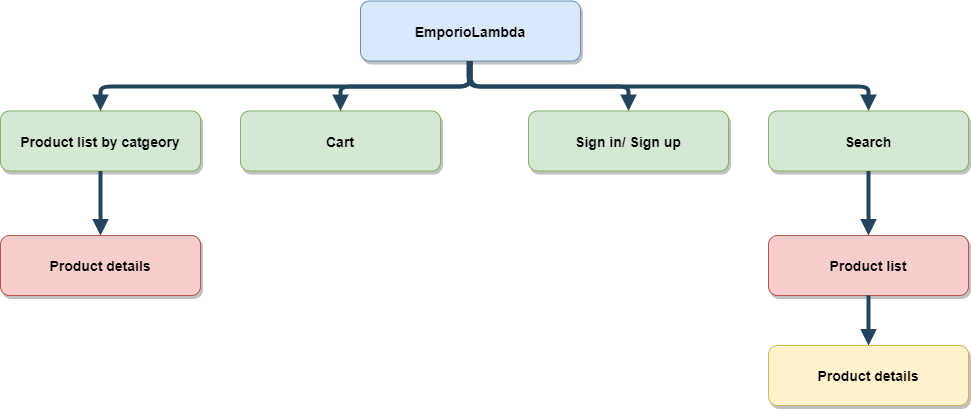
\includegraphics[scale=0.40]{res/ResocontoAttivitaDiVerifica/res/metriche/grafici/img/mappaSitoEsterno.png}\\
\caption{Mappa del sito relativa ad un utente non autenticato}
\end{figure}

\begin{figure}[H]
\centering
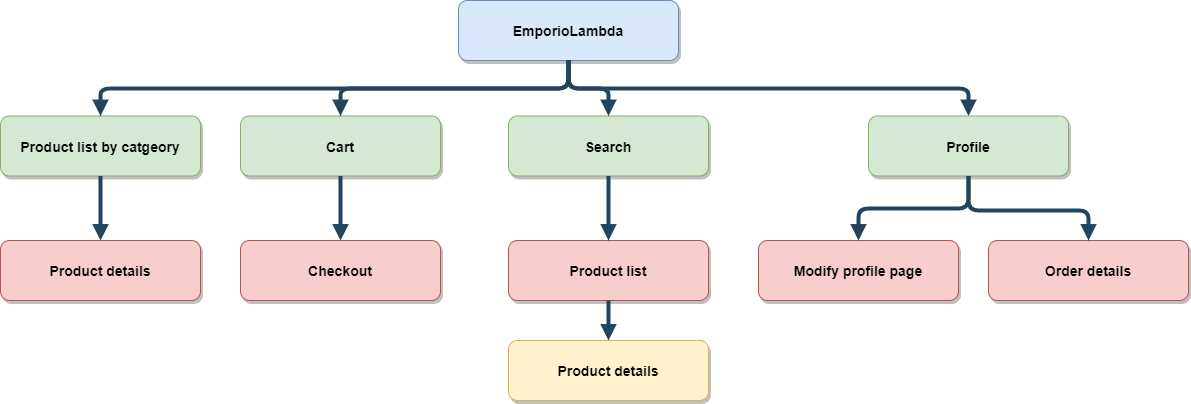
\includegraphics[scale=0.35]{res/ResocontoAttivitaDiVerifica/res/metriche/grafici/img/mappaSitoCliente.png}\\
\caption{Mappa del sito relativa ad un utente cliente}
\end{figure}

\begin{figure}[H]
\centering
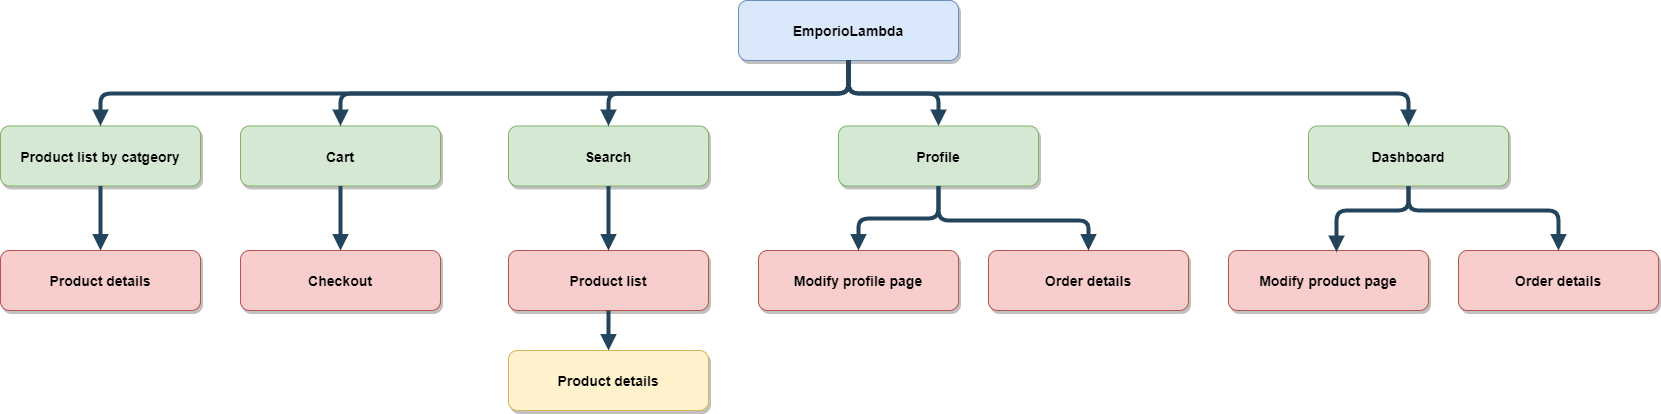
\includegraphics[scale=0.27]{res/ResocontoAttivitaDiVerifica/res/metriche/grafici/img/mappaSitoMerchant.png}\\
\caption{Mappa del sito relativa ad un utente venditore}
\end{figure}

\begin{figure}[H]
\centering
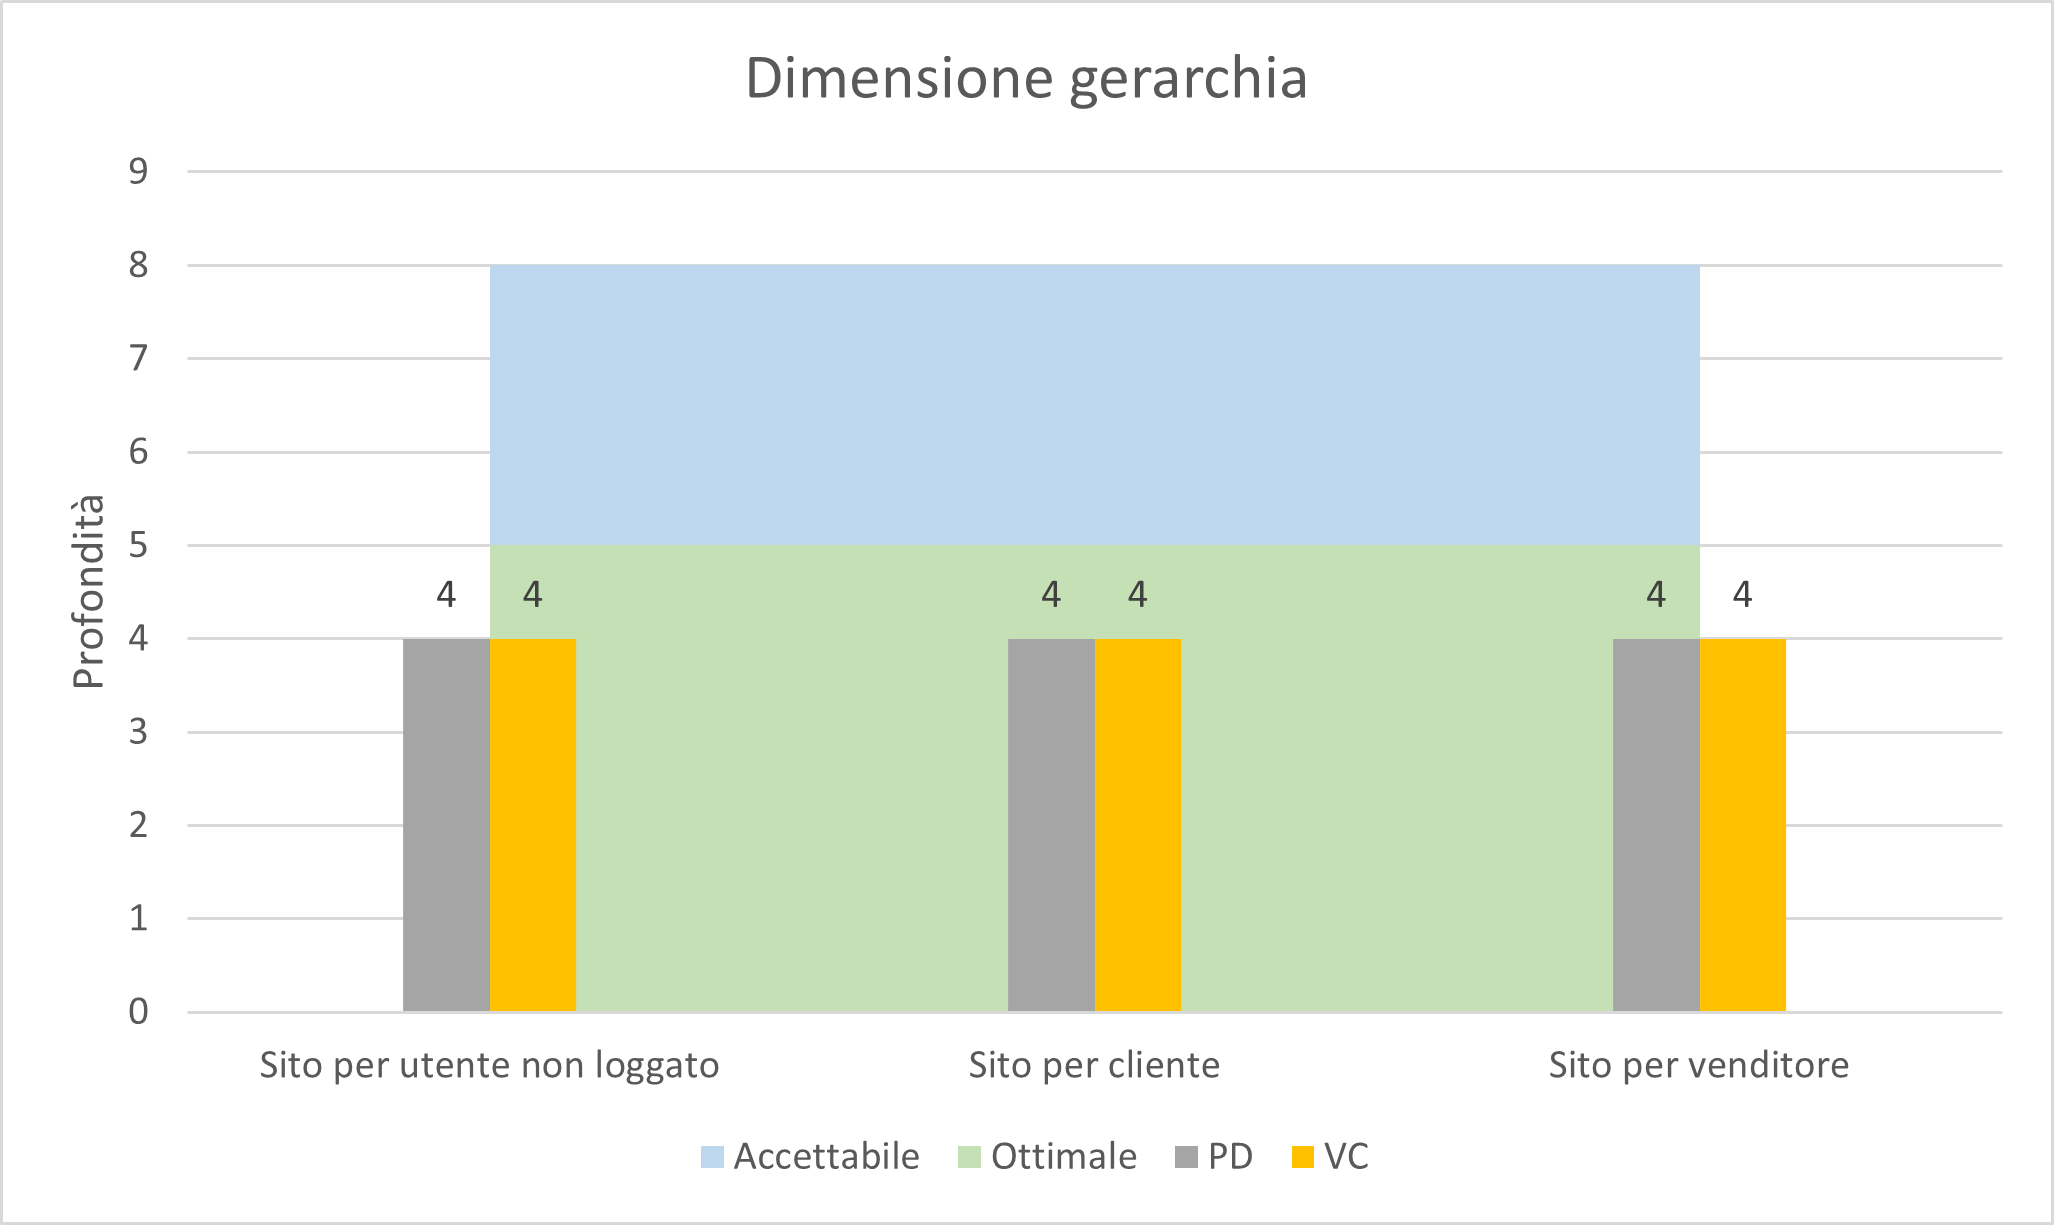
\includegraphics[scale=0.78]{res/ResocontoAttivitaDiVerifica/res/metriche/grafici/img/dimensioneGerarchia.png}\\
\caption{Andamento della profondità della mappa del sito}
\end{figure}

\subsubsection{MPD6 - Facilità di comprensione}
Di seguito sono riportati i grafici della facilità di comprensione relativi al modulo Back-end e Front-end, i cui valori sono definiti accettabili e ottimali come descritto nella sezione §3.4.2.1.\\

\begin{figure}[H]
\centering
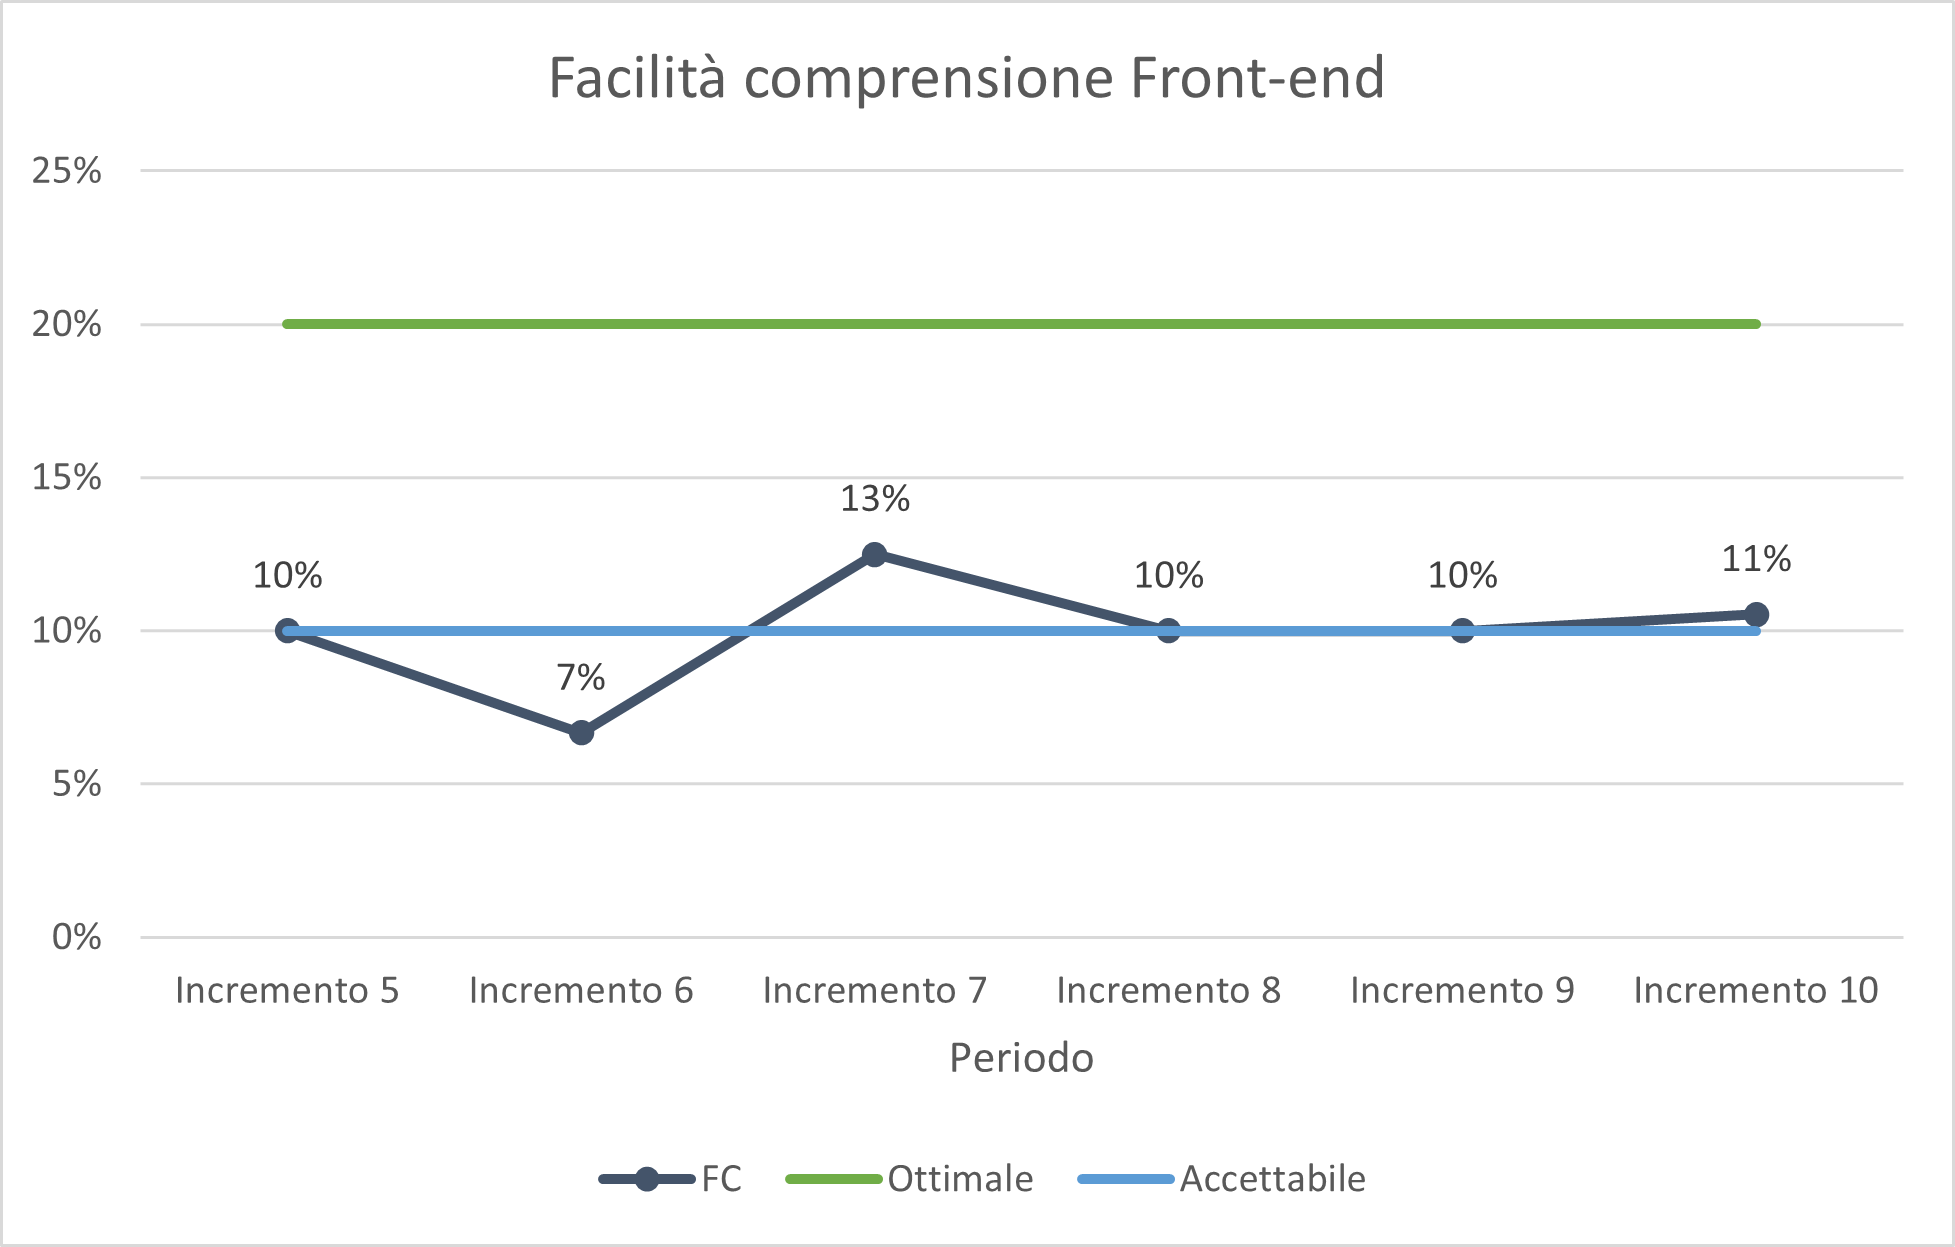
\includegraphics[scale=0.78]{res/ResocontoAttivitaDiVerifica/res/metriche/grafici/img/FCFE.png}\\
\caption{Andamento facilità di comprensione relativo al modulo Front-end}
\end{figure}

\begin{figure}[H]
\centering
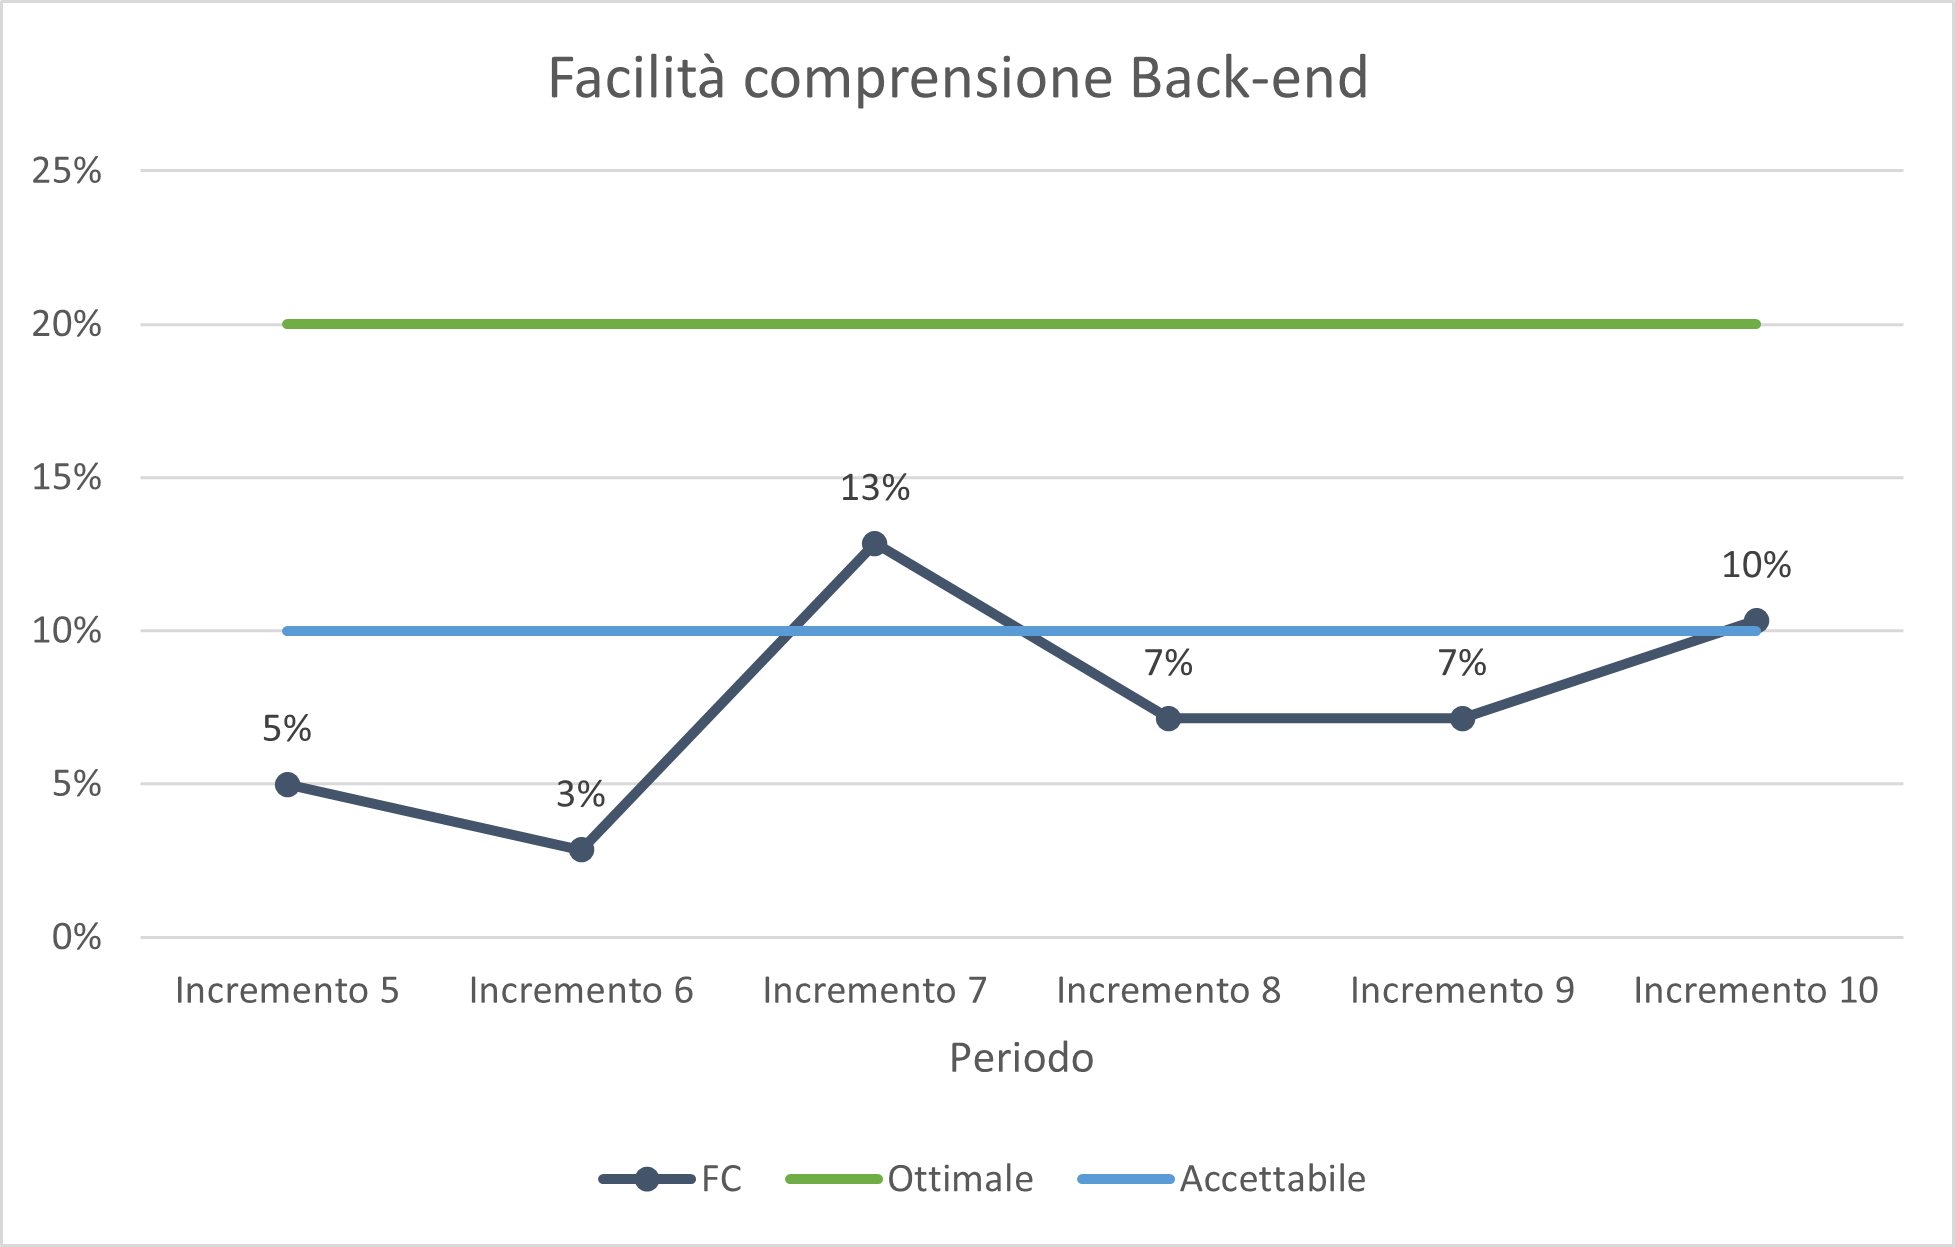
\includegraphics[scale=0.78]{res/ResocontoAttivitaDiVerifica/res/metriche/grafici/img/FCBE.png}\\
\caption{Andamento facilità di comprensione relativo al modulo Back-end}
\end{figure}


\subsubsection{MPD7 - Semplicità classi}
Di seguito sono riportati i grafici della semplicità delle classi relative al modulo Back-end e Front-end, i cui valori sono definiti accettabili e ottimali come descritto nella sezione §3.4.2.2.\\

\begin{figure}[H]
\centering
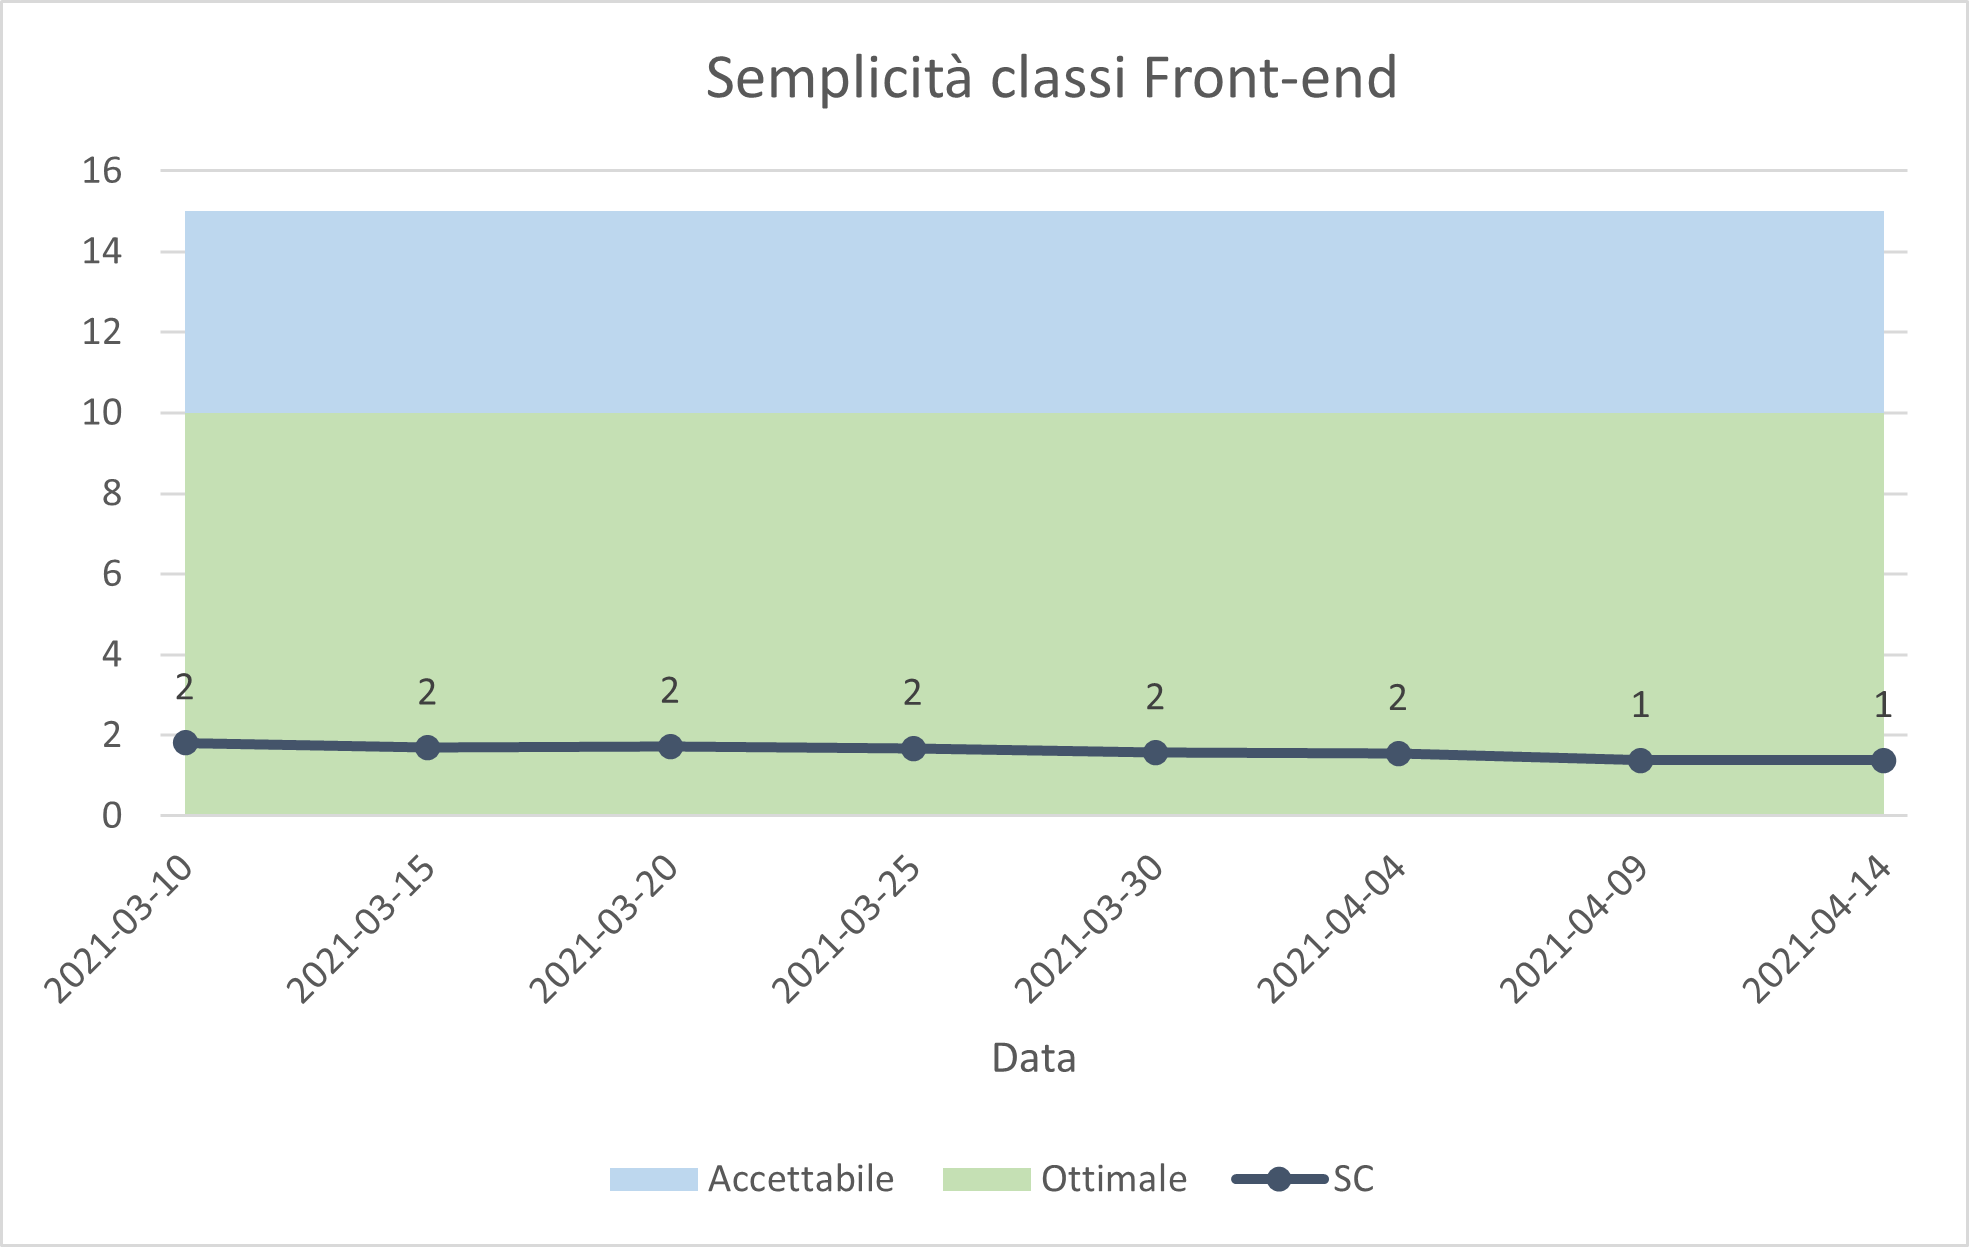
\includegraphics[scale=0.78]{res/ResocontoAttivitaDiVerifica/res/metriche/grafici/img/SCFE.png}\\
\caption{Andamento semplicità delle classi relativo al modulo Front-end}
\end{figure}

\begin{figure}[H]
\centering
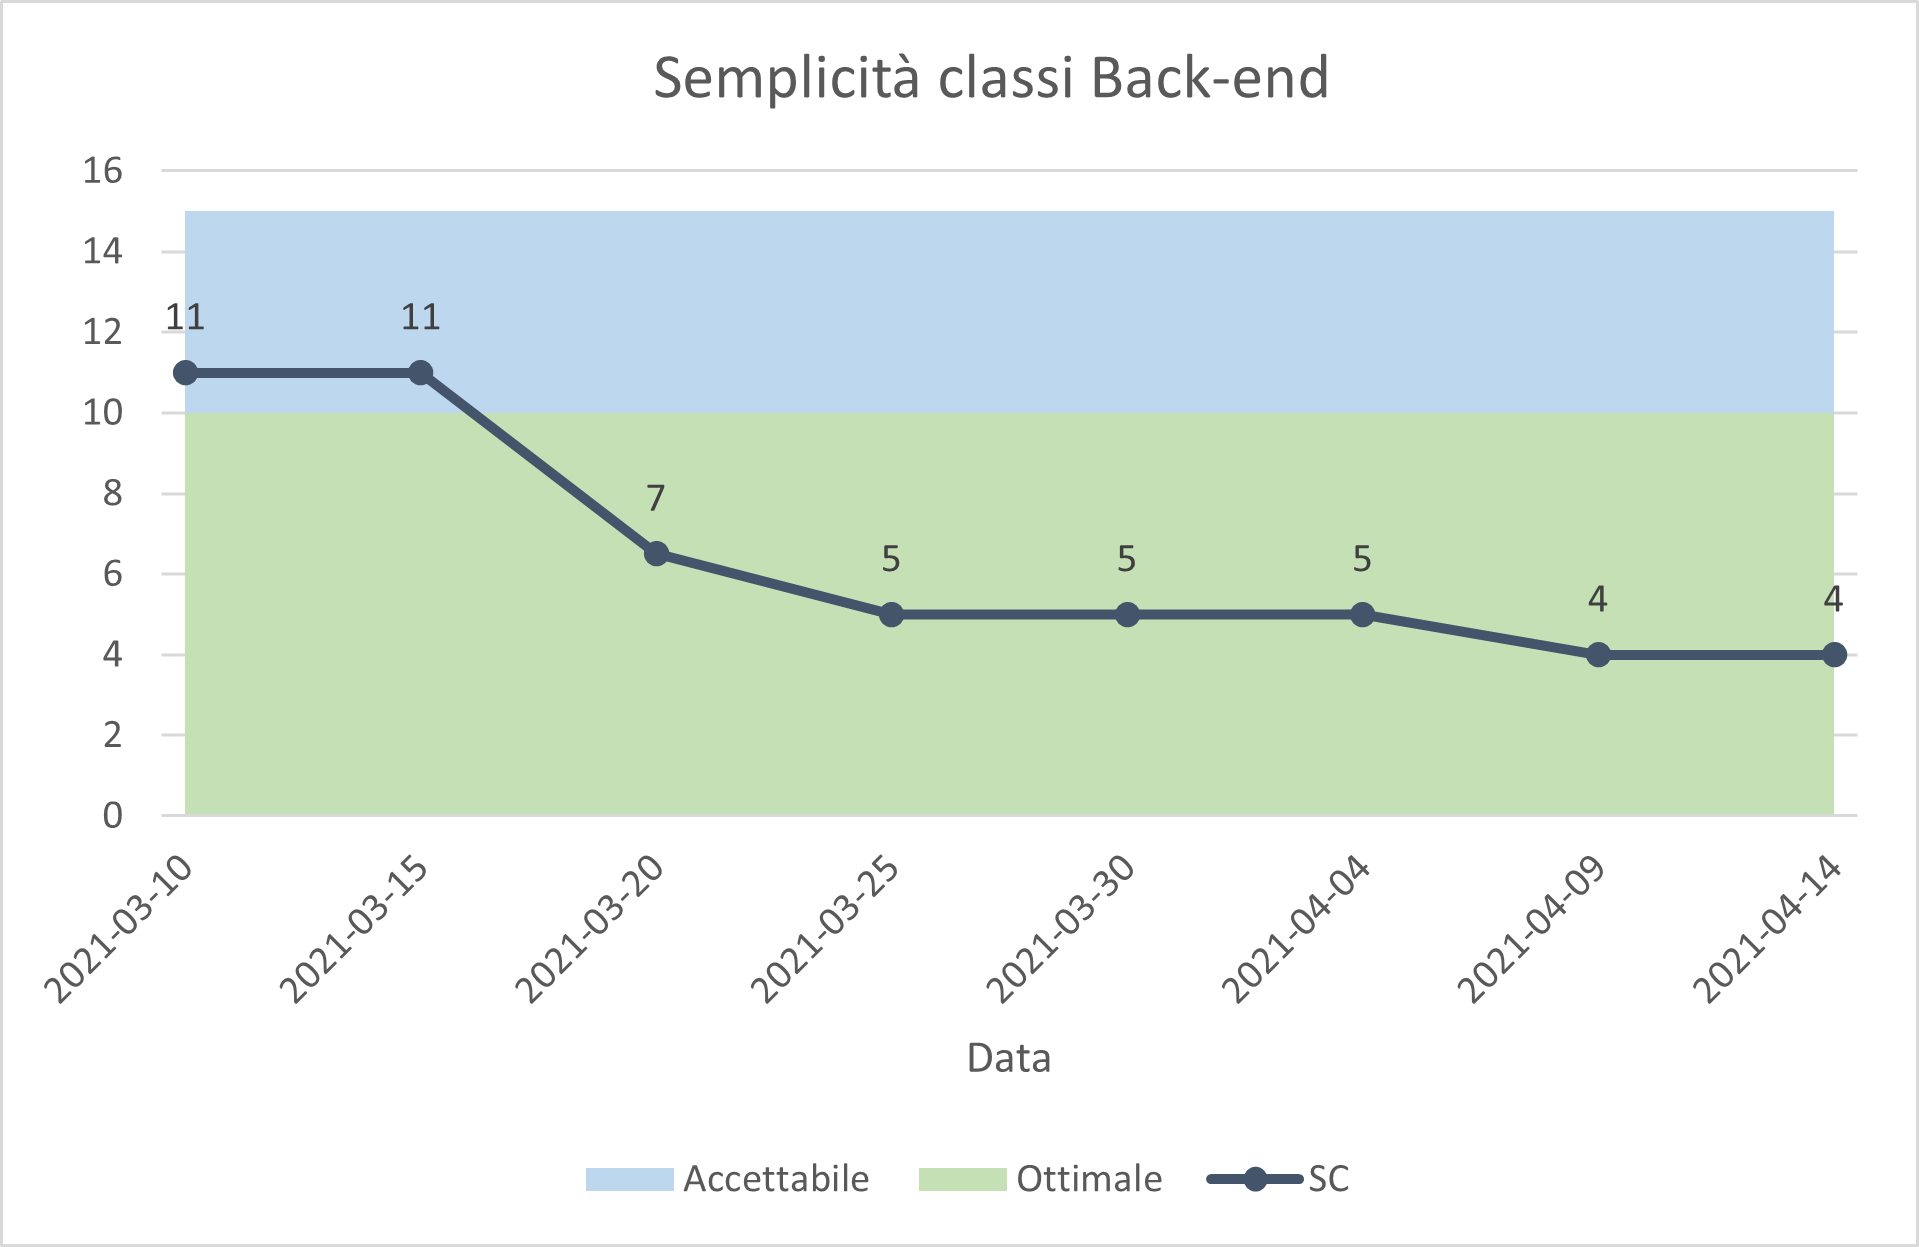
\includegraphics[scale=0.78]{res/ResocontoAttivitaDiVerifica/res/metriche/grafici/img/SCBE.png}\\
\caption{Andamento semplicità delle classi relativo al modulo Back-end}
\end{figure}

\subsubsection{MPD8 - Semplicità funzioni}
Di seguito sono riportati i grafici della semplicità delle funzioni relative al modulo Back-end e Front-end, i cui valori sono definiti accettabili e ottimali come descritto nella sezione §3.4.2.3.\\

\begin{figure}[H]
\centering
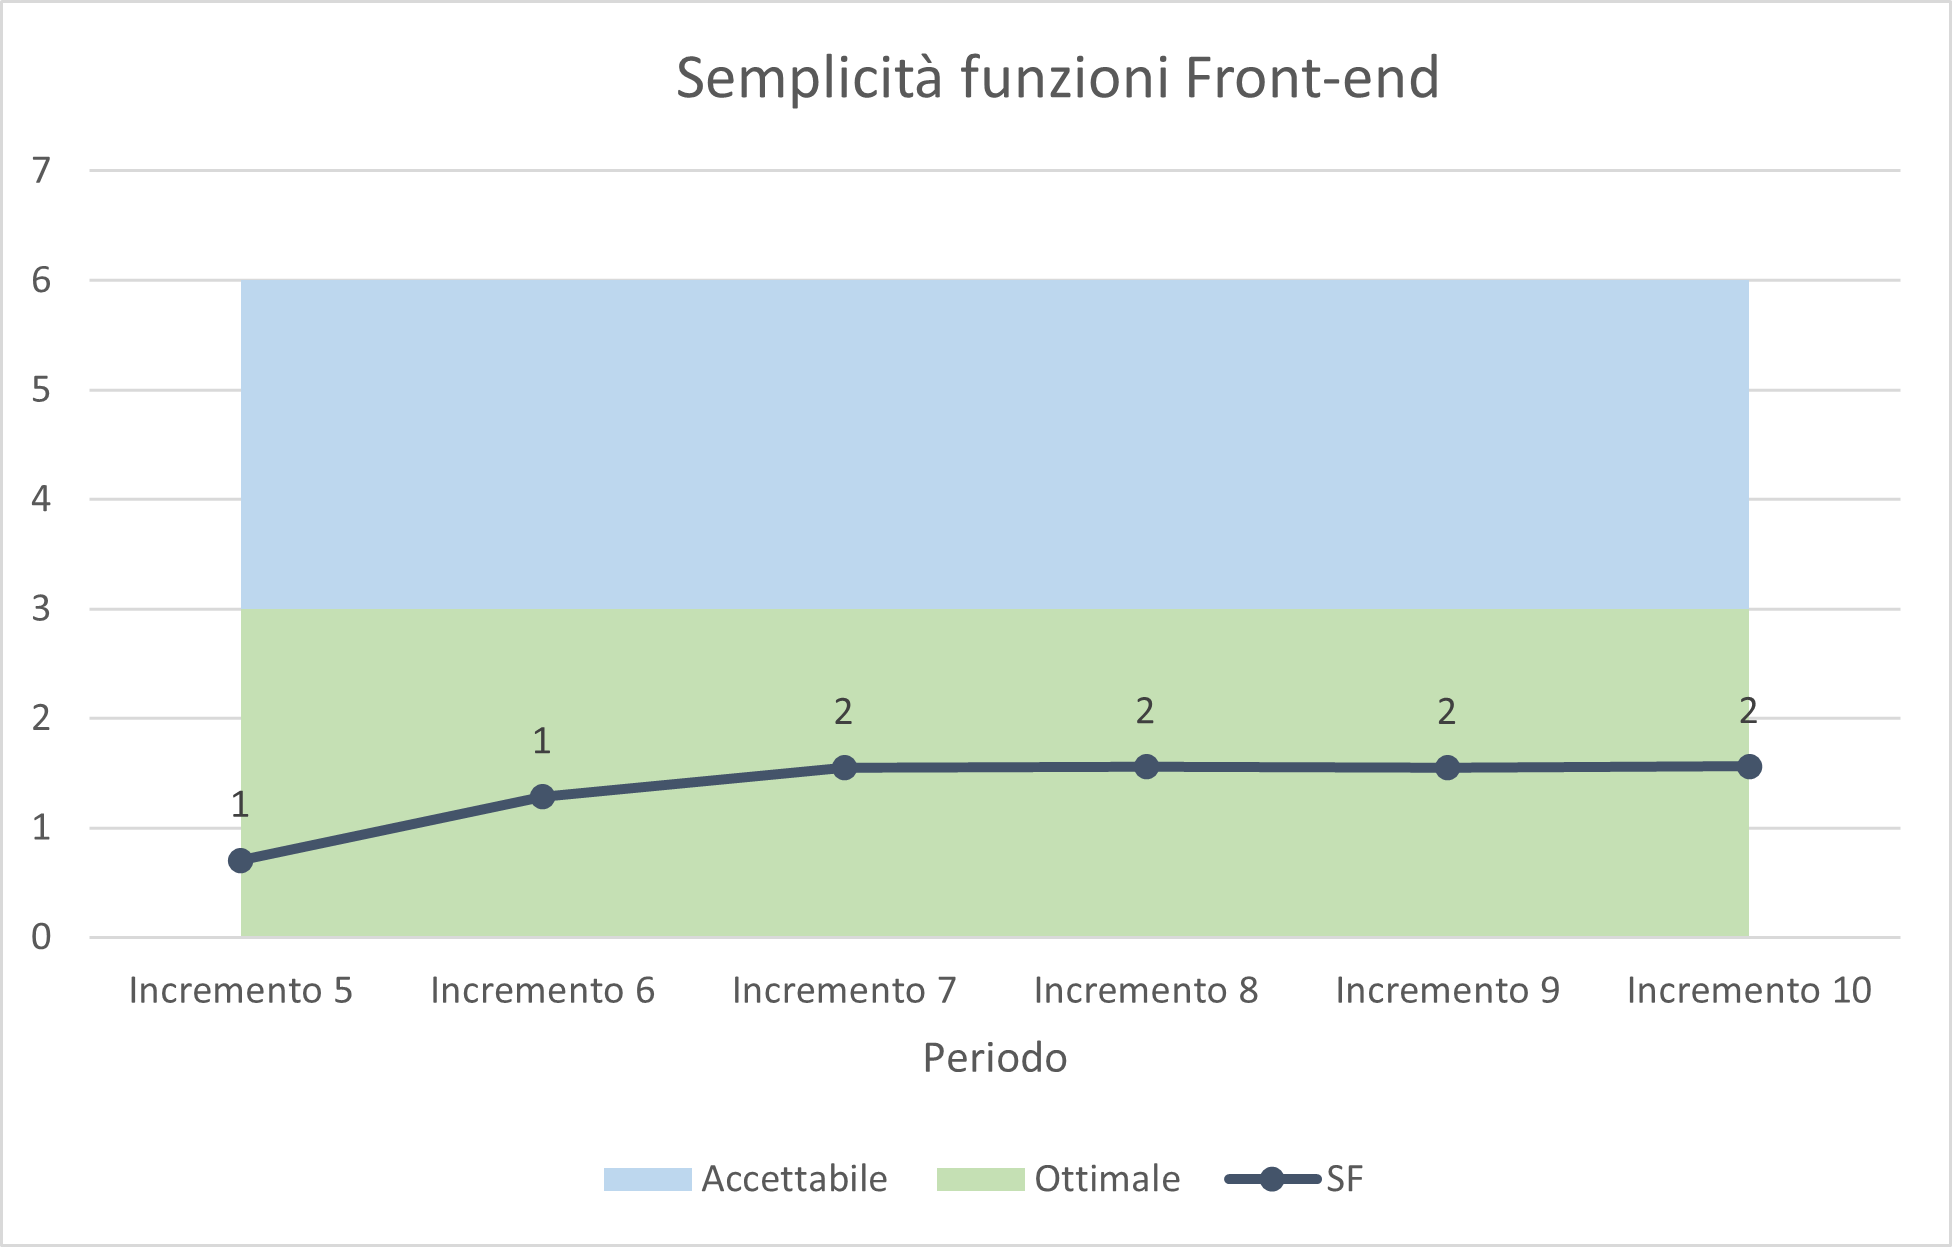
\includegraphics[scale=0.78]{res/ResocontoAttivitaDiVerifica/res/metriche/grafici/img/SFFE.png}\\
\caption{Andamento semplicità delle funzioni relativo al modulo Front-end}
\end{figure}

\begin{figure}[H]
\centering
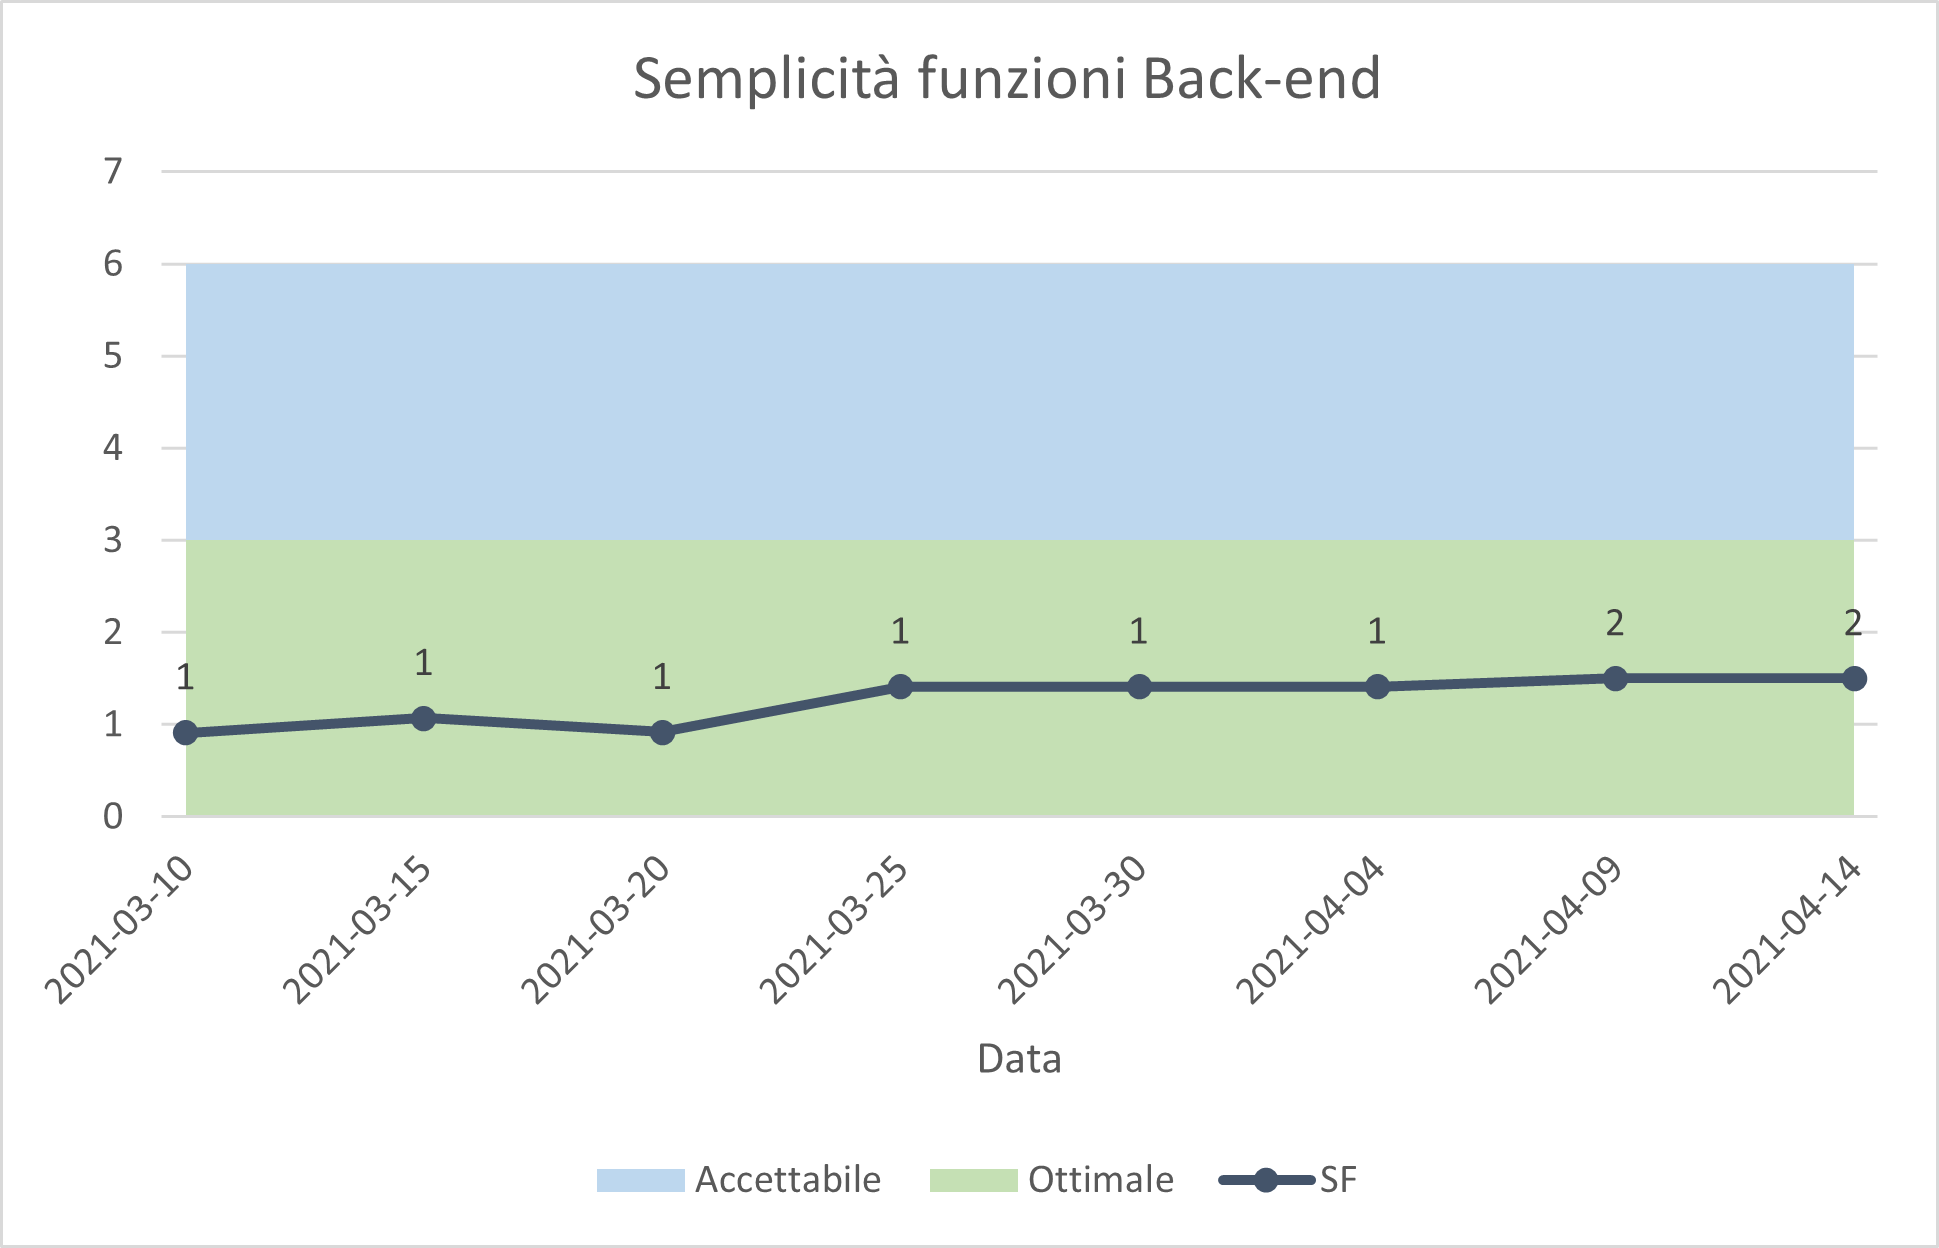
\includegraphics[scale=0.78]{res/ResocontoAttivitaDiVerifica/res/metriche/grafici/img/SFBE.png}\\
\caption{Andamento semplicità delle funzioni relativo al modulo Back-end}
\end{figure}


\subsubsection{MTS1 - Copertura dei requisiti da parte dei test}
Di seguito viene riportato il grafico della copertura dei requisiti da parte dei test, il cui valore è definito accettabile e ottimale come descritto nella sezione §4.1\\

\begin{figure}[H]
\centering
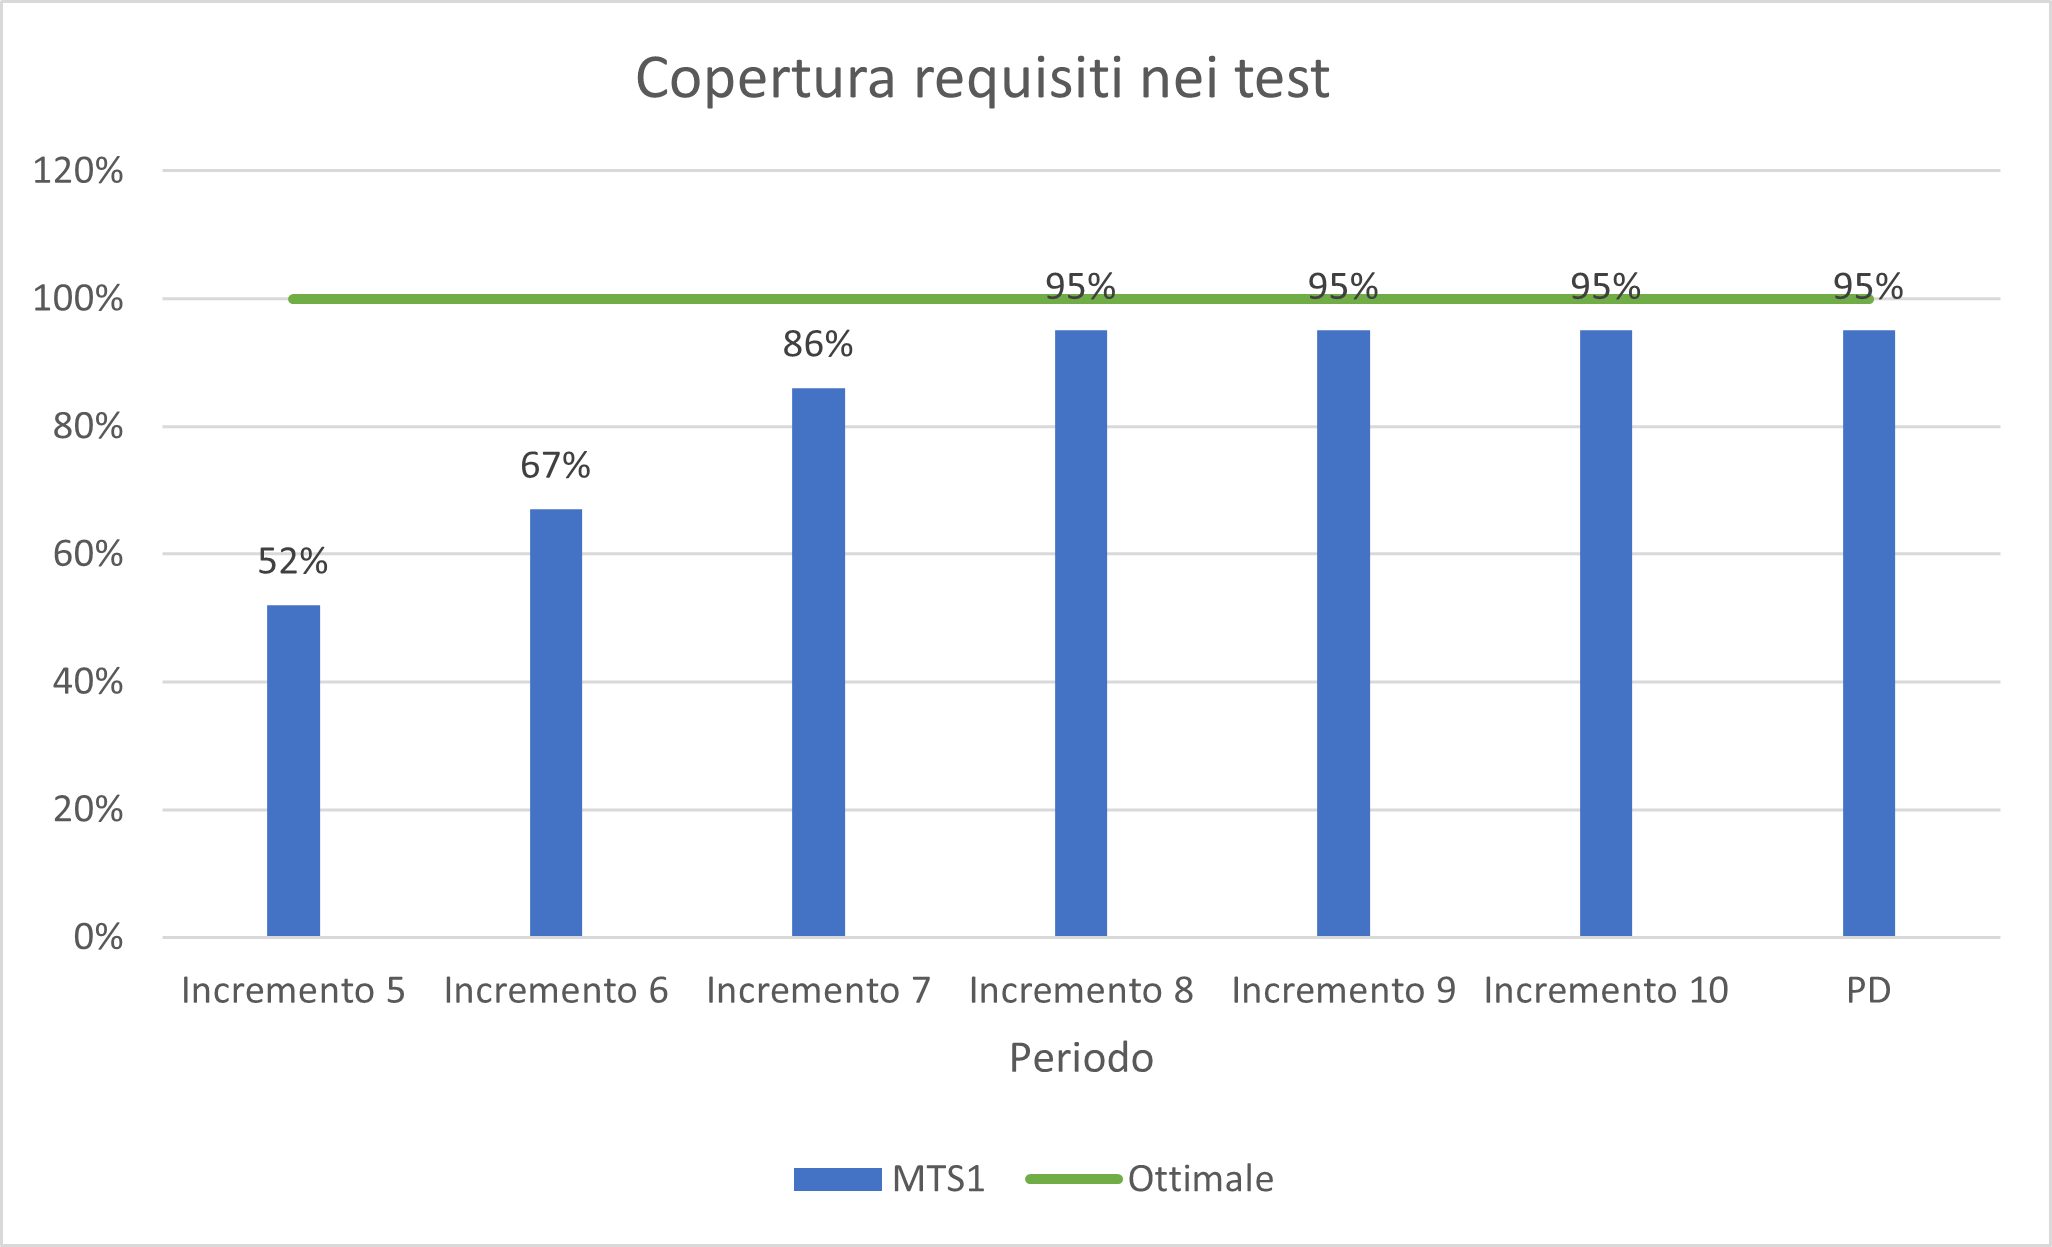
\includegraphics[scale=0.78]{res/ResocontoAttivitaDiVerifica/res/metriche/grafici/img/MTS1.png}\\
\caption{Andamento copertura dei requisiti da parte dei test}
\end{figure}


\subsubsection{MTS2 - Percentuale test passati}
Di seguito viene riportato il grafico della percentuale dei test passati, il cui valore è definito accettabile e ottimale come descritto nella sezione §4.1\\

\begin{figure}[H]
\centering
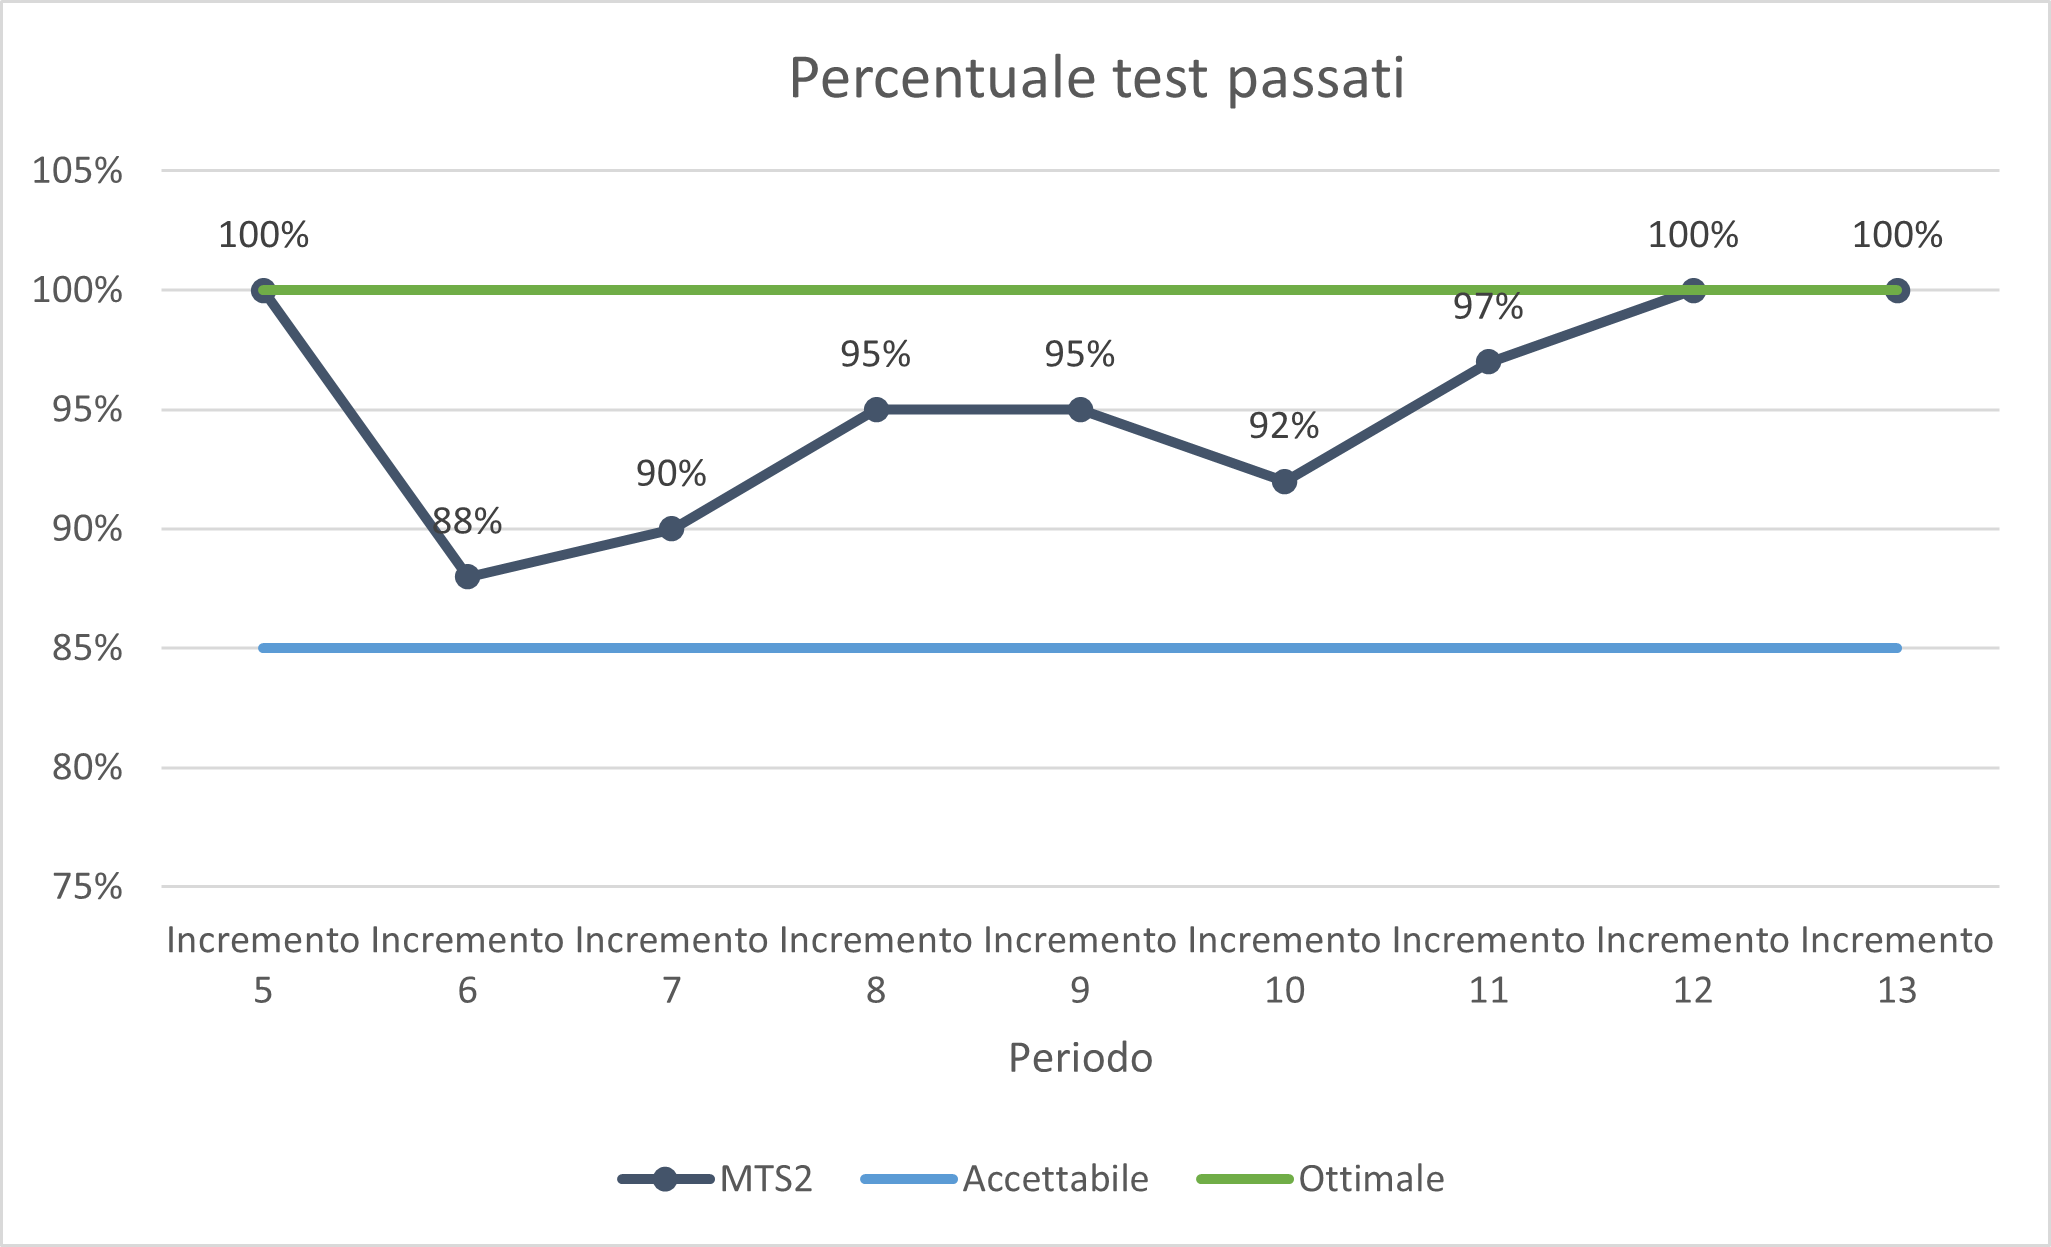
\includegraphics[scale=0.78]{res/ResocontoAttivitaDiVerifica/res/metriche/grafici/img/MTS2.png}\\
\caption{Andamento percentuale test passati}
\end{figure}

